	% ----------------------------------------------------------------------
%                   LATEX TEMPLATE FOR PhD THESIS
% ----------------------------------------------------------------------

% based on Harish Bhanderi's PhD/MPhil template, then Uni Cambridge
% http://www-h.eng.cam.ac.uk/help/tpl/textprocessing/ThesisStyle/
% corrected and extended in 2007 by Jakob Suckale, then MPI-CBG PhD programme
% and made available through OpenWetWare.org - the free biology wiki

%: Style file for Latex
% Most style definitions are in the external file PhDthesisPSnPDF.
% In this template package, it can be found in ./Latex/Classes/
\documentclass[twoside,11pt]{Latex/Classes/PhDthesisPSnPDF}


%: Macro file for Latex
% Macros help you summarise frequently repeated Latex commands.
% Here, they are placed in an external file /Latex/sMacros/MacroFile1.tex
% An macro that you may use frequently is the figuremacro (see introduction.tex)
\include{Latex/Macros/MacroFile1}



%: ----------------------------------------------------------------------
%:                  TITLE PAGE: name, degree,..
% ----------------------------------------------------------------------
% below is to generate the title page with crest and author name

%if output to PDF then put the following in PDF header
\ifpdf  
    \pdfinfo { /Title  (Semantically-enabled Browsing of Large Multilingual Document Collections)
               /Creator (TeX)
               /Producer (pdfTeX)
               /Author (Carlos Badenes-Olmedo cbadenes@fi.upm.es)
               /CreationDate (D:YYYYMMDDhhmmss)  %format D:YYYYMMDDhhmmss
               /ModDate (D:YYYYMMDDhhmm)
               /Subject (xyz)
               /Keywords (document similarity, topic models, large scale, semantic annotation) }
    \pdfcatalog { /PageMode (/UseOutlines)
                  /OpenAction (fitbh)  }
\fi

  
\title{Semantically-enabled Browsing of Large Multilingual Document Collections}


% ----------------------------------------------------------------------
% The section below defines www links/email for author and institutions
% They will appear on the title page of the PDF and can be clicked
\ifpdf
 
  \author{{\hspace{16mm} Carlos Badenes-Olmedo }}
  \supervisor{{ \hspace{5mm} Prof. Dr. Oscar Corcho}}
%  \cityofbirth{born in XYZ} % uncomment this if your university requires this
%  % If city of birth is required, also uncomment 2 sections in PhDthesisPSnPDF
%  % Just search for the "city" and you'll find them.
%  \collegeordept{{Departamento de Inteligencia Artificial \\ Facultad de Inform\'atica}}  
%  \university{\href{http://www.upm.es}{Universidad Polit\'ecnica de Madrid}}  
  % The crest is a graphics file of the logo of your research institution.
  % Place it in ./0_frontmatter/figures and specify the width
%  \crest{\includegraphics[width=3cm]{escudofi.pdf}}
\crest{  
 		\begin{tabular}{l c}
			\multirow{4}{*}{\includegraphics[width=2cm]{intro/figures/escudofi.pdf}} & \\
			& \textbf{Departamento de Inteligencia Artificial} \\ 
			& \textbf{Escuela T\'ecnica Superior de Ingenieros Inform\'aticos} \\
			& \\
		\end{tabular}
}
% If you are not creating a PDF then use the following. The default is PDF.
\else
  \author{YourName}
%  \cityofbirth{born in XYZ}
  \collegeordept{CollegeOrDept}
  \university{University}
  \crest{\includegraphics[width=4cm]{logo}}
\fi

%\renewcommand{\submittedtext}{change the default text here if needed}
\degree{Philosophi\ae Doctor (PhD), DPhil,..}
\degreedate{xxx, 2021}


% Packages ----------------------------------------------------------------------
       
% turn of those nasty overfull and underfull hboxes
\hbadness=10000
\hfuzz=50pt

%\usepackage[]{algorithm2e}
%\usepackage[scaled=0.85]{beramono}
%\usepackage[super]{nth}
%\usepackage[T1]{fontenc}
%\usepackage[table,xcdraw]{xcolor}
\usepackage{adjustbox}
\usepackage[titletoc]{appendix}
%\usepackage{algpseudocode}
\usepackage{amsfonts}
\usepackage{amsmath}
\usepackage{amssymb}
\usepackage{amsthm}
\usepackage{array}
\usepackage{booktabs}
\usepackage{caption}
%\usepackage{changepage}
%\usepackage{color, colortbl}
\usepackage[shortlabels]{enumitem}
\usepackage{float}
\usepackage{graphicx}
\usepackage{hyperref}
\usepackage{listings}
%\usepackage{mathabx}
%\usepackage{mdwlist}
%\usepackage{multicol}
\usepackage{multirow}
%\usepackage{natbib}
%\usepackage{paralist}
%\usepackage{pbox}
%\usepackage{program}
%\usepackage{rotating}
\usepackage{subcaption}
%\usepackage{subfig}
%\usepackage{subfigure}
\usepackage{tabularx}
%\usepackage{textcomp}
%\usepackage{titlesec}
\usepackage{url}
%\usepackage{verbatim}
\usepackage[table]{xcolor}

%\usepackage{todonotes}

\newenvironment{conditions}[1][where:]
  {#1 \begin{tabular}[t]{>{$}l<{$} @{${}={}$} l}}
  {\end{tabular}\\[\belowdisplayskip]}

\newcolumntype{b}{X}
\newcolumntype{s}{>{\hsize=.6\hsize}X}
\newcolumntype{H}{>{\raggedright\arraybackslash}X}
\newcolumntype{S}{>{\centering\hsize=.6\hsize}X}
\newcolumntype{C}{>{\centering\arraybackslash}X} % centered version of 'X' col. type
\newcommand{\heading}[1]{\multicolumn{1}{c}{#1}}

\lstset{language=SQL, morekeywords={PREFIX,java,rdf,rdfs,url,dbpr,owl,umbel,FILTER}}
\setcounter{secnumdepth}{2}
\setcounter{tocdepth}{2}


\definecolor{codegreen}{rgb}{0,0.6,0}
\definecolor{codegray}{rgb}{0.5,0.5,0.5}
\definecolor{codepurple}{rgb}{0.58,0,0.82}
\definecolor{backcolour}{rgb}{0.95,0.95,0.92}
\lstdefinestyle{mystyle}{
    backgroundcolor=\color{backcolour},   
    commentstyle=\color{codegreen},
    keywordstyle=\color{magenta},
    numberstyle=\tiny\color{codegray},
    stringstyle=\color{codepurple},
    basicstyle=\footnotesize,
    breakatwhitespace=false,         
    breaklines=true,                 
    captionpos=b,                    
    keepspaces=true,                 
    numbers=left,                    
    numbersep=5pt,                  
    showspaces=false,                
    showstringspaces=false,
    showtabs=false,                  
    tabsize=2
}
\lstset{style=mystyle}


\definecolor{Gray1}{gray}{0.85}
\definecolor{Gray2}{gray}{0.92}

\definecolor{lightgray}{gray}{0.97}
\definecolor{mediumgray}{gray}{0.94}

\usepackage{chngcntr}
\counterwithout{footnote}{chapter}


\DeclareCaptionFormat{algor}{%
  \hrulefill\par\offinterlineskip\vskip1pt%
    \textbf{#1#2}#3\offinterlineskip\hrulefill}
\DeclareCaptionStyle{algori}{singlelinecheck=off,format=algor,labelsep=space}
%\captionsetup[algorithm]{style=algori}

\pdfoptionpdfminorversion 6

% -------------
%  PARTIAL COMPILATION
% \includeonly{firstbit,lastbit}
% -------------

%\includeonly{hypothesis/hypothesis}

%: --------------------------------------------------------------
%:                  FRONT MATTER: dedications, abstract,..
% --------------------------------------------------------------

\begin{document}

%\language{english}

% sets line spacing
\renewcommand\baselinestretch{1.2}
\baselineskip=18pt plus1pt

\theoremstyle{plain}
\newtheorem{thm}{Theorem}[chapter] % reset theorem numbering for each chapter

\theoremstyle{definition}
\newtheorem{defn}[thm]{Definition} % definition numbers are dependent on theorem numbers

\newcommand{\attention}[1]{{\color{red}\textbf{#1}}}
\newcommand{\comm}[1]{{\color{red}(Comment:#1)}}
\newcommand{\duda}[1]{{\color{red}(DUDA:#1)}}

\renewcommand\appendixname{ANNEX}


%: ----------------------- generate cover page ------------------------
\frontmatter
\maketitle  % command to print the title page with above variables


%: ----------------------- cover page back side ------------------------
% Your research institution may require reviewer names, etc.
% This cover back side is required by Dresden Med Fac; uncomment if needed.

%\newpage
\pagestyle{plain}
\cleardoublepage
\pagestyle{plain}

\noindent Tribunal nombrado por el Sr. Rector Magfco. de la Universidad Polit\'{e}cnica de
Madrid, el d\'{i}a XX de xxx de 2021.

\vspace{10mm}
Presidente:\hspace{0.3mm} Dr. Horacio Saggion

\vspace{5mm}
Vocal: \hspace{6.7mm} Dr. Raphaël Troncy

\vspace{5mm}
Vocal: \hspace{6.7mm} Dr. Jerónimo Arenas García

\vspace{5mm}
Vocal: \hspace{6.7mm} Dr. Jose Manuel Gómez Pérez

\vspace{5mm}
Secretario:\hspace{0.65mm} Dr. Victor Rodriguez Doncel

\vspace{5mm}
Suplente: \hspace{1.5mm} Dra. Elena Montiel Ponsoda

\vspace{5mm}
Suplente: \hspace{1.5mm} Dr. Mariano Fernandez López

\vspace{10mm}
\noindent Realizado el acto de defensa y lectura de la Tesis el d\'{i}a X de xxx de 2021 en la Escuela T\'ecnica Superior de Ingenieros Inform\'aticos

\vspace{5mm}
\noindent Calificaci\'{o}n: \rule{123mm}{0.2mm}
\vspace{20mm}

EL PRESIDENTE \hspace{30mm} VOCAL 1 \hspace{30mm} VOCAL 2

\vspace{30mm}
%\begin{center}
\hspace{15mm} VOCAL 3 \hspace{45mm} EL SECRETARIO
%\end{center}

%EL PRESIDENTE \hspace{60mm} LOS VOCALES
%
%\vspace{30mm}
%\begin{center}
%EL SECRETARIO
%\end{center}



%: ----------------------- acknowledgement ------------------------

\cleardoublepage
% Thesis Dedication ---------------------------------------------------

\begin{dedication} %this creates the heading for the dedication page

\hfill A mis padres. \\
\hfill A Beatriz. \\
\hfill A Martín y Alonso.

\end{dedication}

% ----------------------------------------------------------------------

\cleardoublepage
% Thesis Acknowledgements ------------------------------------------------


%\begin{acknowledgementslong} %uncommenting this line, gives a different acknowledgements heading
\begin{acknowledgements}      %this creates the heading for the acknowlegments

Although I didn't know it yet, this journey began almost 10 years ago in Boston, with Susana Muñoz. A study about the Ivory Coast, a presentation at M.I.T. and a strong determination to continue learning. New plans and a new future. Oscar Corcho then appeared, and thanks to him everything started to take shape. I discovered science in the Ontology Engineering Group, with great researchers who are also great colleagues. Asunción Gómez, Jorge Gracia, Victor Fernandez, Raul Garcia, Elena Montiel, Mariano Fernandez, Jose Angel Ramos and Mariano Rico. Particularly impressive were the talks with María Poveda, Dani Vila and Julia Bosque. New ideas and unforeseen approaches came up in every talk. I admire you. Research means reading, understanding, testing and also collaborating. I am very grateful for the interactions with Daniel Garijo, Filip Radulovic and Idafen Santana, with Pablo Calleja and Rafael Gonzalez, with Nandana Mihindukulasooriya and Freddy Priyatna, with Esteban Gonzalez and with Fernando Serena, and the dedicated support of Raul Alcazar and Miguel Angel, because you forced me to be more pragmatic. And I cannot forget the DiversiTeam, where all the extra skills are put into practice. I don't want to forget anyone, you are all part of this work: David Chaves, Paola Espinoza, Francisco Yedro, Alba Fernandez, Maria Navas, Patricia Martin, Elvira Amador, Edna Ruckhaus, Alvaro Brandon, Serge Chavez, Andres Prados, Ana Iglesias, and Julian Arenas.

Special mention for my supervisor, Oscar Corcho, and my mentor, Jose Luis Redondo. Both of you have the ability to choose the right words and simplify any task. You have complemented each other perfectly, even from the distance, and I have enjoyed every year of this thesis. Oscar knows how to touch the right keys at the right time, and Jose Luis reduces each problem to the challenge that motivates it, no matter how complex it was. I am extremely lucky to have you by my side on this journey, and and your influence will guide my future steps.

Thank you so much Beatriz for offering me so much help this time. These have been very intense years, with many changes and challenges, but we have been able to keep smiling and move forward. I hope Martin and Alonso feel proud of us for having achieved our objectives. I will miss our nights working with their crying in the background.

Federico and Loli, I had imagined it otherwise, but I know you will be proud of me. Not for the thesis, but for the decisions that led me to do it. You are in everything I do, and thanks to your effort this achievement has become a reality. I also have to thank the patience of my sisters, Ana and Lucia, who have always been able to push me forward.



\end{acknowledgements}
%\end{acknowledgementslong}

% ------------------------------------------------------------------------




%: ----------------------- abstract ------------------------

\cleardoublepage

% Thesis Abstract -----------------------------------------------------


\begin{abstractslong}  
%english
xxxxx
\end{abstractslong}

\cleardoublepage
\begin{abstractslongSpanish}
%spanish
xxxxxx

\end{abstractslongSpanish}
% ---------------------------------------------------------------------- 


%: ----------------------- index ------------------------
\cleardoublepage
\setcounter{secnumdepth}{3} % organisational level that receives a numbers
\setcounter{tocdepth}{3}    % print table of contents for level 3

\tableofcontents           % print the table of contents

% levels are: 0 - chapter, 1 - section, 2 - subsection, 3 - subsection


%: ----------------------- list of figures/tables ------------------------

\listoffigures	% print list of figures

\listoftables  % print list of tables

%: ----------------------- glossary ------------------------

% Tie in external source file for definitions: /0_frontmatter/glossary.tex
% Glossary entries can also be defined in the main text. See glossary.tex

% this file is called up by thesis.tex
% content in this file will be fed into the main document

%: ----------------------- introduction file header -----------------------
\chapter{Acronyms } \label{ch:acronyms}

\graphicspath{{intro/figures/}}

% -------------------------------------------------------------
% ----------------------- Chapter intro ----------------------- 
% -------------------------------------------------------------


\begin{description}
\itemsep0em
	\item[AI:] Artificial Intelligence
	\item[AIES:] Advances In Engineering Software journal dataset
	\item[ANN:] Approximate Nearest Neighbour
	\item[API:] Application Programming Interface
	\item[BoW:] Bag-of-Words
	\item[CHHM:] Centroid-based Hierarchical Hashing
	\item[CRDC:] Cumulative Ranking on Dirichlet distribution- based Clustering 
	\item[DHHM:] Density-based Hierarchical Hashing
	\item[DR:] Document Retrieval
	\item[DRM:] Dirichlet Random Mixture dataset
	\item[HE:] Hellinger Distance
	\item[IR:] Information Retrieval
	\item[JS:] Jensen Shannon divergence
	\item[KL:] Kullback-Liebler divergence
	\item[LDA:] Latent Dirichlet Allocation
	\item[LSA:] Latent Semantic Analysis
	\item[LSH:] Locality-Sensitive Hashing
	\item[MAP:] Mean Average Precision
	\item[MuPTM:] Multilingual Probabilistic Topic Model
	\item[NLP:] Natural Language Processing
	\item[NM:] Neural Models
	\item[PLSA:] Probabilistic Latent Semantic Analysis
	\item[PTM:] Probabilistic Topic Model
	\item[RDC:] Ranking on Dirichlet distribution-based Clustering
	\item[TDC:] Trends on Dirichlet distribution-based Clustering
	\item[TF:] Term Frequency
	\item[TF-IDF:] Term Frequency-Inverse Document Frequency
	\item[THHM:] Threshold-based Hierarchical Hashing
	\item[URI:] Uniform Resource Identifier
	\item[URL:] Uniform Resource Locator
	\item[VSM:] Vector Space Models
	\item[WUI:] Web User Interface
\end{description}









 

%: --------------------------------------------------------------
%:                  MAIN DOCUMENT SECTION
% --------------------------------------------------------------

% the main text starts here with the introduction, 1st chapter,...

\mainmatter

%: ----------------------- subdocuments ------------------------


% this file is called up by thesis.tex
% content in this file will be fed into the main document

%: ----------------------- introduction file header -----------------------
\chapter{Introduction}\label{ch:introduction}

\graphicspath{{introduction/figures/}}

% -------------------------------------------------------------
% -- Introduction
% -------------------------------------------------------------

% Motivation: 
% - Presentar el problema general y las soluciones propuestas por la tesis (enfoque top-down), en vez del enfoque técnico actual (bootom-up)
% - Buscar referencias que hablen del número de docs que se generan cada día, o cosas similares
% - Hablar de knowledge-intensive task, o de knowledge-workers, o similar

%%% <-- present the motivation

% huge data (https://www.nature.com/articles/nj7612-457a)
% large-scale
% Around 8 TB of textual data are consumed everyday by electronic media. 
% https://curia.europa.eu/jcms/upload/docs/application/pdf/2020-05/ra_pan_2019_interieur_en_final.pdf
Huge amounts of textual documents are produced daily in digital format. More than two thousand blog entries are published, nine thousand tweets are written, and more than two million emails are sent on the Internet every second in 2021\footnote{https://www.internetlivestats.com/one-second}. The number of scientific publications per year  increased by 8-9\%~in the last decade \citep{Ware2018STM}. More than one million papers, about two per minute,  were submitted to the PubMed database, the leading database of references and abstracts on life sciences and biomedical research, during 2018. The behavior is similar in other domains. More than 168,000 procedural documents and 3,000 judicial notices were published in the Official Journal of the European Union\footnote{\url{https://eur-lex.europa.eu/oj/direct-access.html}} in 2019. Furthermore, unlike the academic domain where articles are mostly published in English, legal documents are usually available in multiple languages. The Court of Justice of the European Union\footnote{\url{https://curia.europa.eu}} had to translate in 2019 over 1 million texts into its 24 official languages, with 552 possible language combinations, in just one year. These numbers make it difficult for an expert in the academic or legal domains to stay abreast by only reading a few articles nowadays. Navigating the growing torrent of textual data and exploring their content is not only necessary, but has become a crucial activity that experts must add to their daily tasks. 

Document retrieval techniques are being used nowadays to facilitate text review in such big collections. Major digital publishers specialized in scientific\footnote{\url{https://www.nature.com}}, technical\footnote{\url{https://www.elsevier.com}}, and medical\footnote{\url{https://pubmed.ncbi.nlm.nih.gov}} content provide search engines that make it easier to browse their collections of digital articles. Given a few keywords, a list of relevant papers is retrieved and offered for reading. Legal documents are also exploited through similar solutions. The Spanish\footnote{\url{https://www.oepm.es}}, American\footnote{\url{https://www.uspto.gov/}} and European\footnote{\url{https://www.epo.org}} intellectual property registration offices, for example, allow exploring their patent collections by search engines guided by keywords and/or categories. These categories are based on the International Patent Classification (IPC) system and are available thanks to the manual annotation of their authors and of patent officers. This classification contains approximately 70,000 codes for different technical areas. This label-based browsing has been also adopted by other academic search engines\footnote{\url{https://academic.microsoft.com}} to organize papers by research areas, or even by evaluation tasks to cover the state-of-the-art methods\footnote{\url{https://paperswithcode.com}}. A domain such as natural language processing, for example, is organized into 256 categories such as 'knowledge representation', 'question-answering', 'machine translation' and so on. However, the use of tags to categorize scientific papers is still insufficient and some additional text processing tasks are required to homogenize the format and criteria of the article labels. One of the main reasons that limits a widespread use is the \textit{difficulty to identify labels that describe a research work in sufficient detail}.

% A new research field or category appear?
Furthermore, not all approaches can assume that new categories will emerge. \textit{Searches guided by keywords or tags are useful when the domain is known, but when new categories appear these mechanisms are insufficient}. In scientific domains, a way to identify new research areas is through peer review processes. There are also reports that identify the hottest and emerging specialty areas in scientific research from the last years\footnote{\url{https://discover.clarivate.com/ResearchFronts2019_EN}}. The methodology used in these reports assumes that cumulatively, and over time, citations in research leave a trail that highlights progress and advancements across a range of fields. By regularly tracking these citations and unpacking the patterns and groupings of how papers are cited, in particular clusters of papers that are frequently cited together, new research areas take shape. Such reports also exist on patent collections to discover technology trends\footnote{\url{https://www.wipo.int/tech_trends}}.

In this context, identifying relationships between documents is key to know their information and facilitate their exploration. A documentary exploration does not stop when a relevant article is found, but starts from its content shaping the area of interest through its relations. Most academic\footnote{\url{https://www.semanticscholar.org}} and legal\footnote{\url{https://patents.google.com}} search engines provide a list of related documents for each text and offer navigating through them. The relationship between two documents can be based on references, when documents are cited by others\footnote{\url{http://citationgecko.com}}, or content, when documents share a thematic area. The chains of articles derived from that related content can lead to more complex structures when cross-relations are considered. A document can be related to another that, in turn, is related to a third one that can be also related to the first article. This content-guided exploration helps browsing document collections by areas of interest not necessarily aligned with a list of predefined categories. A visual overview of an academic field, for example, can be provided by showing graphs of articles with similar content\footnote{\url{https://www.connectedpapers.com}}.

While these initiatives are valuable efforts to address access to huge amounts of documents, they are still insufficient to make the most out of the knowledge available within the textual collection. Two types of inferences are needed: \textit{bottom-up}, from documents to collections, and \textit{top-down}, from document relationships to texts. The knowledge derived from a text comes from the concepts evoked by its words \citep{Griffiths2007}, and the knowledge derived from a document collection emerges from the relationships between its texts \citep{Kenter2015}. Both require understanding the meaning, the semantics, of texts at different levels. \textit{Semantic awareness is desirable to interpret the relationships and guide the exploration}. The focus is on why some texts are related and what concepts are key to those relationships. But analyzing and comparing texts on a large scale also requires addressing some challenges imposed by external conditions that have appeared in recent years:
\begin{itemize}
\item \textbf{Complexity}: The increasing variety of themes, in ever growing collections, has forced a reconsideration of the way to compare their documents. The operations required to compute each comparison should be simplified as much as possible.
\item \textbf{Efficiency}: The algorithms, besides being accurate enough, must be also efficient in order to be applied on a large scale. Brute-force techniques cannot be applied to compare all items in a huge corpus.
\item \textbf{Explainability}: The relations among documents must be explained in such a way that provide knowledge about the content of the texts. It is not enough that one text is related to another, it is necessary to explain why it is so. 
\item \textbf{Multilinguality}: The increasing availability of texts written in different natural languages also makes it necessary to address comparison in multilingual collections. External translation systems cannot been considered as the only applicable solution, since they increase processing costs and potentially introduce a bias in the relationships that are obtained. Solutions that relate texts without translating them are desirable.
\end{itemize}

In our work we aim at \textbf{facilitating the exploration of huge collections of documents written in multiple languages}. We address the problem of comparing them on a large scale while enabling a semantic-aware exploration through their content. Our proposal automatically discovers thematic associations between texts using probabilistic models to describe their content through topics, and organizes document collections so that they can be efficiently and transparently browsed through the related content regardless of their language.

\section{Contributions}

The following contributions are presented in this thesis:

\begin{itemize}
\item \textbf{A Scalable Framework for Probabilistic Topic Modeling}: We design and implement a text processing model that supports the creation of probabilistic topic models by distributing operations among functional units. Based on this abstraction, we implement a framework that becomes the foundation of this thesis research, which is used as a tool for supporting performance analysis and algorithm design.
\item \textbf{A Publishing Model for Probabilistic Topic Models}: We propose a unified form to publish and (re)use topic models as Web services that are available from online repositories, so as to facilitate the exploitation of probabilistic topic models.
\item \textbf{Hierarchical Thematic Annotations for High-dimensional Topic Models}: To study the problem of representativeness in high dimensional topic models, we exploit the relationships between texts derived from their topic distributions. We show how the distances vary between the same texts when the dimensions of the model change, and how less representative topics can influence their calculation. Our analytical and experimental results show that \textit{the more topics are available in the model, the less representative are the distance measurements based on densities}. We identify hierarchies in the topic distributions that maintain their representativeness regardless of the dimensionality of the model, and without losing the ability to measure distances. We propose a method to annotate texts using topic hierarchies, and a distance metric based on these hierarchical representations.
\item \textbf{Support for Large-scale Document Similarity Comparisons}: We present an efficient mechanism to index and retrieve related documents using hierarchical annotations. It facilitates the exploration of a collection by the themes inferred from its texts.
\item \textbf{Identify Cross-lingual Document Relations}: We introduce a technique to transform probabilistic topics from different languages into a single representation space based on shared concepts where texts can be thematically related regardless of the language used.
\end{itemize}

\section{Thesis Structure}

The thesis is structured as follows:

\textit{Chapter \ref{ch:soa}} describes the main concepts handled throughout the thesis, analyses the state of the art and identifies the main limitations. \textit{Chapter \ref{ch:hypothesis}} presents the research problems and hypotheses that guide our work, as well as assumptions and restrictions and details the methodology that has been followed in this research. \textit{Chapter \ref{ch:scalability}} describes the software architecture proposed to analyze huge document collections and the format suggested to distribute and reuse the topic models built in this thesis. \textit{Chapter \ref{ch:explainability}} details our proposed text annotation algorithm to organize probabilistic topics into hierarchical levels according to their relevance. \textit{Chapter \ref{ch:comparisons}} shows how to store and search documents efficiently from large collections when they are annotated with topic hierarchies.  \textit{Chapter \ref{ch:multilinguality}} explains the method to relate multilingual texts from their main topics without requiring any prior knowledge between the languages. \textit{Chapter \ref{ch:experiments}} describes real-world projects where the results from this thesis have been used. Finally, \textit{Chapter \ref{ch:conclusion}} presents the conclusions and introduce the future lines of work. Where relevant, evaluations have been included in the corresponding chapters where the specific contributions are presented.


\section{Publications}

The following publications support the research work presented in this thesis:

% relacionar los papers a los capítulos, en vez de orden cronológico.

\begin{itemize}
\item \textbf{Chapter \ref{ch:scalability}: Creation and Publication of Probabilistic Topic Models}:
\begin{itemize}
\item \textit{\textbf{Carlos Badenes-Olmedo}, José Luis Redondo-Garcia, and Oscar Corcho. \textit{Distributing Text Mining tasks with librAIry}. Proceedings of the 17th ACM Symposium on Document Engineering (DocEng). Association for Computing Machinery, Valletta, Malta. 2017.} This is the key paper describing the architecture and technological features of librAIry, our framework for processing texts and creating probabilistic topic models. 
\item \textit{Victoria Kosa, Alyona Chugunenko, Eugene Yuschenko, \textbf{Carlos Badenes-Olmedo}, Vadim Ermolayev, and Aliaksandr Birukou. \textit{Semantic saturation in retrospective text document collections}. Information and Communication Technologies in Education, Research, and Industrial Applications (ICTERI) PhD Symposium, vol. 1851, pages 1-8. CEUR-WS. 2017.} The work presented in this paper makes use of the text-processing module proposed by librAIry to retrieve multi-word terms from a document collection.
\item \textit{Victoria Kosa, David Chaves-Fraga, Dmitriy Naumenko, Eugene Yuschenko, \textbf{Carlos Badenes-Olmedo}, Vadim Ermolayev, Aliaksandr Birukou, Nick Bassiliades, Hans-Georg Fill, Vitaliy Yakovyna, Heinrich C. Mayr, Mykola Nikitchenko, Grygoriy Zholtkevych, and Aleksander Spivakovsky. \textit{Cross-Evaluation of Automated Term Extraction Tools by Measuring Terminological Saturation}. Information and Communication Technologies in Education, Research, and Industrial Applications, pages 135-163. Springer International Publishing. 2018.} The distributed document processing and representation model used by librAIry is improved during this work to support the extraction of the most relevant terms from a collection of scientific articles.
\end{itemize}
\item \textit{Chapter \ref{ch:explainability}- Explainable Topic-based Associations}:
\begin{itemize}
\item \textbf{Carlos Badenes-Olmedo}, José Luis Redondo-García, and Oscar Corcho. \textit{Efficient Clustering from Distributions over Topics}. Proceedings of the 9th International Conference on Knowledge Capture (K-CAP), Article 17, 1–8. Association for Computing Machinery, Austin, TX, USA. 2017. This article provides the basis for transforming probabilistic topic distributions into expressions that group similar content. 
\item \textbf{Carlos Badenes-Olmedo}, Jose Luis Redondo-Garcia, and Oscar Corcho. \textit{An initial Analysis of Topic-based Similarity among Scientific Documents based on their Rhetorical Discourse Parts}. Proceedings of the 1st Workshop on Enabling Open Semantic Science (SemSci) co-located with 16th International Semantic Web Conference (ISWC 2017), 15-22. Vienna, Austria. 2017. This work demonstrates the need to use full texts to relate content from their topic distributions, since the use of abstracts of scientific texts is shown to be less accurate than other longer sections. 
\end{itemize}
\item \textbf{Chapter \ref{ch:comparisons}: Large-scale Comparisons of Topic Distributions}:
\begin{itemize}
\item \textit{\textbf{Carlos Badenes-Olmedo}, José Luis Redondo-García, and Oscar Corcho. \textit{Large-scale Semantic Exploration of Scientific Literature Using Topic-based Hashing Algorithms}. Semantic Web, vol. 11, no. 5, pp. 735-750. 2020.} This paper describes the key algorithm of this thesis to reduce probabilistic topic distributions into hierarchical expressions that relate similar content without losing topic information.
%\item Borja Lozano, \textbf{Carlos Badenes-Olmedo} and Oscar Corcho. Hierarchical representations of topics to uncover the underlying knowledge of semantically related texts. Proceedings of the 22nd International Conference on Knowledge Engineering and Knowledge Management (EKAW), (under revision). 2020
\end{itemize}
\item \textbf{Chapter \ref{ch:multilinguality}: Cross-lingual Document Similarity}:
\begin{itemize}
\item \textit{\textbf{Carlos Badenes-Olmedo}, José Luis Redondo-García, and Oscar Corcho. \textit{Scalable Cross-lingual Document Similarity through Language-specific Concept Hierarchies}. Proceedings of the 10th International Conference on Knowledge Capture (K-CAP). Association for Computing Machinery, 147–153. Marina Del Rey, CA, USA. 2019.} In this paper we describe probabilistic topics using concept-based representations instead of words.  Multilingual topics are automatically aligned to create a single representation space across languages.   
\item \textit{\textbf{Carlos Badenes-Olmedo}, José Luis Redondo-García, and Oscar Corcho. \textit{Legal document retrieval across languages: topic hierarchies based on synsets}. Proceedings of the 1st Workshop on Iberlegal co-located with 32nd International Conference on Legal Knowledge and Information Systems organized by the Foundation for Legal Knowledge Based Systems (JURIX). Madrid, Spain. 2019.} The work presented in this paper evaluates the conceptual representation of multilingual topics to relate legal documents in several languages: English, Spanish, French and Portuguese.
\end{itemize}
\item \textbf{Chapter \ref{ch:experiments}: Experiments}:
\begin{itemize}
\item \textit{Beatriz López-Centeno, \textbf{Carlos Badenes-Olmedo}, Ángel Mataix-Sanjuan, Katie McAllister, José M Bellón, Sara Gibbons, Pascual Balsalobre, Leire Pérez-Latorre, Juana Benedí, Catia Marzolini, Ainhoa Aranguren-Oyarzábal, Saye Khoo, María J Calvo-Alcántara, Juan Berenguer. \textit{Polypharmacy and Drug-Drug Interactions in People Living With Human Immunodeficiency Virus in the Region of Madrid, Spain: A Population-Based Study}. Clinical Infectious Diseases. vol. 71,2, 353-362. 2020.} In this work we exploit the ability of librAIry to relate content described by hierarchical representations. In a medical domain, patients are grouped according to the drugs used in their treatments and their potential interactions.
\item \textit{Ahmet Soylu, Oscar Corcho, Brian Elvesaeter, \textbf{Carlos Badenes-Olmedo}, Francisco Yedro, Matej Kovacic, Matej Posinkovic, Ian Makgill, Chris Taggart, Elena Simperl, Till C. Lech, and Dumitru Roman. \textit{Enhancing Public Procurement in the European Union through Constructing and Exploiting an Integrated Knowledge Graph}. Proceedings of the 19th International Semantic Web Conference (ISWC). 2020.} This paper presents the work done to relate multilingual European regulations to public contracts through their hierarchical topic-based representations. A document search engine that leverages this facility is built.  
\item \textit{\textbf{Carlos Badenes-Olmedo}, David Chaves-Fraga, Maria Poveda-Villalon, Ana Iglesias-Molina, Pablo Calleja, Socorro Bernardos, Patricia Martín-Chozas, Alba Fernández-Izquierdo, Elvira Amador-Dominguez, Paola Espinoza-Arias, Luis Pozo, Edna Ruckhaus, Esteban Gonzalez-Guardia, Raquel Cedazo, Beatriz Lopez-Centeno, and Oscar Corcho. \textit{Drugs4Covid: Drug-driven Knowledge Exploitation based on Scientific Publications}. arXiv e-prints:2012.01953. 2020.} In the context of creating a knowledge graph describing the drugs used to treat COVID-19, this article shows the work to adapt librAIry to infer relationships between drugs from their mentions in scientific articles. 
\end{itemize}
\end{itemize}



	

% this file is called up by thesis.tex
% content in this file will be fed into the main document

%: ----------------------- introduction file header -----------------------
\chapter{State of the Art}\label{ch:soa}

\graphicspath{{soa/figures/}}

% -------------------------------------------------------------
% -- Related Work
% -------------------------------------------------------------

In this chapter the main concepts that will be used throughout the rest of the thesis are introduced. 
We analyze the current state of the art and limitations in the area of exploration of large and multilingual document collections. First, the tasks derived from processing the texts and enabling a semantic-aware exploration of the corpus are described. Then, an overview of the existing methods that perform these tasks is introduced. And finally, for each research area involved, the limitations that must be addressed to achieve the ultimate goal of facilitating documentary exploration are presented. 

\section{Information Retrieval}

The analysis of human-readable documents is a well-known problem in Artificial Intelligence (AI) in general, and in the Information Retrieval (IR) and Natural Language Processing (NLP) fields in particular. As an academic field of study, information retrieval might be defined as finding documents of an unstructured nature, usually text, that satisfies an information need from within large collections \citep{manning2008}. As defined in this way, hundreds of millions of people engage in information retrieval every day when they use a web search engine or search their email. Information retrieval is fast becoming the dominant form of information access, surpassing traditional database searching where identifiers are needed to have results. 

There are some key concepts in this area.  The  records  that  IR  addresses  are  called \textit{documents}, and they are retrieved from an organized repository, most commonly called  \textit{collection} or \textit{corpus}. It is not restricted to static collections. The collection may be a stream of texts, e.g., scientific publications, patents, news dispatches, that are created periodically. DR focuses on retrieving documents from a collection based on their content. A request, typically called a \textit{query},  may specify desired characteristics of the documents to be retrieved, e.g., \textit{The documents should be about ‘Text Similarity’ and their author must be ‘Badenes’}. In this example, the query asks for documents whose content (the \textit{unstructured} part) is \textit{about} a certain topic and whose author (a \textit{structured} part) has a specified value. 

\textit{Unstructured Content} means that there is no well-defined syntax for a given document, let alone a syntax that all documents share. To the extent that documents share a syntax, there is no well-defined semantics associated with each syntactic component \citep{greengrass2000}. Now, think about how data is \textit{structured} in a database. All records of a given type have the same syntax, e.g., all rows in a table of a relational database will have the same columns \citep{Salton1983}.  Moreover,  each  component  of  a  record  will  have  a  definite meaning (i.e. semantics)  and  a  given  component  of  a  given  record  type  will  have  the  same semantics in every record of that type. The practical effect is that given the name of a component, a search engine can use the syntax to find the given component in a given record and retrieve its contents, its value. Similarly, given a component and a value, the search engine can find records such that the given component contains the given value. For example, a relational database can be asked to retrieve the contents of the \textit{year} column of a \textit{Thesis} table in an \textit{Academic} database. The search engine knows how to find the \textit{Thesis} table within  the  \textit{Academic}  database,  and  how  to  find  the  \textit{year}  column  within  each  record  of  the \textit{Thesis} table.  And  every  \textit{year}  column  within  the  \textit{Thesis}  table  will  have  the  same semantics, i.e., the year of publication of a thesis. 

But the column name \textit{year} may not be sufficient to identify the column. A \textit{Course} table in the same or a different database may also have a \textit{year} column. Hence in general, it may be necessary to specify a path, e.g., database name, table name,column name, to uniquely identify the syntactic component to the search engine. However, the syntax of a well-structured database is such that it is always possible to specify a given syntactic component uniquely and hence it is always possible for the search engine to find all occurrences of a given component. If the given component has a definite semantics, then it is always possible for the search engine to find data with that semantics, e.g., to find the years of all theses. 

By contrast, in a collection of unstructured natural language documents, there is no well-defined syntactic position where a search engine could find data with a given semantics, e.g., the years of theses. In a random collection of documents, there is no guarantee that they are all about the same topic, e.g., theses. Even if it is known that the documents are all about theses, there is no simple well-defined way of knowing where the year occurs in a given document, e.g., in what sentence or even in what paragraph. This is exactly what is meant by \textit{unstructured} texts.

An IR engine may use the query to classify the documents in a collection, returning to the user a subset of documents that satisfy some classification criterion. Documents that satisfy the query are said to be \textit{relevant}. The higher the proportion of documents returned to the user that judges as relevant, the better the classification criterion. Alternatively, the search engine may \textit{rank} the documents in a given collection. Document $D_1$ is higher ranking with respect to a given query $Q$ than document $D_2$, which means that $D_1$ is more likely to satisfy $Q$ than $D_2$. Or it may be interpreted as meaning that $D_1$ satisfies $Q$ more than $D_2$. Two measures of IR success, both based on the concept of relevance, are widely used: \textit{precision} and \textit{recall}. Precision is defined as the ratio of relevant items retrieved to all items retrieved, or the probability given that an item is retrieved that it will be relevant. Recall is defined as, the ratio of relevant items retrieved to all relevant items in a collection, or the probability given that an item is relevant that it will be retrieved \citep{saracevic1995}.

\section{Techniques for Document Retrieval}\label{sec:related-work}

There are two major categories of IR technology and research: semantic and statistical. Semantic approaches attempt to implement some degree of syntactic and semantic analysis. They try to reproduce to some degree the understanding of the natural language text that a human user would provide. In statistical approaches, the documents that are retrieved or that are highly ranked are those that match the query most closely in terms of some statistical measure. The work presented in this thesis follows this second approach. 

Statistical approaches break documents and queries into \textit{terms}. These terms are the population that is counted and measured statistically. Most commonly, the terms are words (or combination of adjacent words or characters) that occur in a given query or collection of documents and often require pre-processing. Words are reduced to a common base form by using a heuristic process that removes affixes, \textit{stemming}, or by returning its dictionary form, \textit{lemma} \citep{porter1997}. The objective is to eliminate the variation that arises from the occurrence of different grammatical  forms  of  the  same  word,  e.g.,  "program",  "programming",  "programs", and "programmed" should all be recognized as forms of the same word, "program". Another common form of pre-processing is the elimination of common words that have little power to discriminate relevant from non-relevant documents,e.g., "the", "a", "it". Hence, IR engines are usually provided with a \textit{stop-list} of such noise words. Note that both stemming/lemma and \textit{stopwords} are language-dependent. Once all terms have been pre-processed, numerical weights are assigned to each them. The same term may have a different weight in each distinct document in which it occurs. The weight is usually a measure of how effective the given term is likely to be in distinguishing the given document from other documents in the given collection, and is often normalized to be a fraction between zero and one. Statistical approaches fall into the following categories: \textbf{\textit{boolean}}, \textbf{\textit{vector space}} and \textbf{\textit{probabilistic}}.

An illustrative example\footnote{\url{https://github.com/cbadenes/phd-thesis/blob/master/notebooks/soa.ipynb}} may help to better understand these techniques. The publications listed in Section \ref{sec:publications} are used as a sample collection for applying information retrieval techniques. Documents are first pre-processed as described above to transform their texts into terms. Typically these terms are referred to as \textit{tokens}. Let's see the process by analyzing the following sentence taken from one of the documents: \textit{"Probabilistic Topic Models reduce that feature space by annotating documents with thematic information"}. Each word, identified using whitespace characters, is normalized using its dictionary form (stemming could also have been performed in this step). The sentence is then transformed into a list of lemmatized words: "\textit{['Probabilistic', 'Topic', 'Models', 'reduce', 'that', 'feature', 'space', 'by', 'annotate', 'document', 'with', 'thematic', 'information']}". Some words have changed and others have remained unchanged. For example, 'annotating' is reduced to 'annotate' and 'documents' to 'document'. However, 'Models' remains unchanged. The reason is that it is considered a proper noun since it starts with a capital letter. Once the words have been normalized, the words with less informative capacity are eliminated (e.g. \textit{'that'}, \textit{'by'} and \textit{'with'}). They usually belong to a stop-word list associated with a given language, but can also be domain-specific. The final list of terms are the tokens used to describe each of the documents.  Table \ref{table:ir-collection} shows the number of words and tokens of each document when preprocessed.


\begin{table}[!htbp]
\centering%
\begin{tabularx}{\linewidth}{lHll}
\toprule
\heading{Id} & \heading{Title} & \heading{Words} & \heading{Tokens} \\
\midrule
\midrule
$D_0$ & Cross-Evaluation of Term Extraction Tools by Measuring Terminological Saturation & 12,954 & 6,342 \\
\midrule
$D_1$ & Enhancing Public Procurement in the European Union through Constructing and Exploiting an Integrated Knowledge Graph & 5,827 & 3,406 \\
\midrule
$D_2$ & Drugs4Covid: Making drug information available from scientific publications & 5,417 & 3,260 \\
\midrule
$D_3$ & Distributing Text Mining tasks with librAIry & 2,448 & 1,477 \\
\midrule
$D_4$ & Large-Scale Semantic Exploration of Scientific Literature using Topic-based Hashing Algorithms & 9,041 & 5,604 \\
\midrule
$D_5$ & An initial Analysis of Topic-based Similarity among Scientific Documents based on their Rhetorical Discourse Parts & 2,641 & 1,425 \\
\midrule
$D_6$ & Efficient Clustering from Distributions over Topics & 5,346 & 2,986 \\
\midrule
$D_7$ & Legal Documents Retrieval Across Languages: Topic Hierarchies based on synsets & 1,445 & 787 \\
\midrule
$D_8$ & Scalable Cross-lingual Document Similarity through Language-specific Concept Hierarchies & 4,602 & 2,963 \\
\midrule
$D_9$ & Potentially inappropriate medications in older adults living with HIV & 3,087 & 2,018 \\
\midrule
$D_{10}$ & Semantic Saturation in Retrospective Text Document Collections & 7,700 & 1,753 \\
\midrule
\bottomrule
\end{tabularx}
\caption{Number of words and tokens of publications listed in Section \ref{sec:publications} when preprocessed.}
\label{table:ir-collection}
\end{table}


%Some sophisticated engines also extract \textit{phrases} as terms. A phrase is a combination of adjacent words which may be recognized by frequency of co-occurrence in a given collection or by presence in a phrase dictionary, e.g. "artificial intelligence". 
%At the other extreme, some engines break documents and queries into \textit{n-grams}, i.e., arbitrary strings of $n$ consecutive characters \citep{damashek1995}. A window of $n$ characters can be moved moved through the entire document, completely ignoring word, phrase, or punctuation boundaries, or can be constrained by word separators, or by other punctuation characters. In any case, since a single word or phrase can generate multiple n-grams, statistical clustering using n-grams has proved to be language-independent, and has even been used to sort documents by language, or by topic within language.

In a \textbf{boolean approach}, the query is formulated as a boolean combination of terms. Documents are reduced to true or false representations for each word depending on whether they contain it or not. A conventional boolean query uses the classical operators AND, OR, and NOT. The query "$t_1$ AND $t_2$" is satisfied by a given document $D_1$ if and only if $D_1$ contains both terms $t_1$ and $t_2$. Similarly, the query "$t_1$ OR $t_2$" is satisfied by $D_1$ if and only if it contains $t_1$ or $t_2$ or both. The query "$t_1$ AND NOT $t_2$" satisfies $D_1$ if and only if it contains $t_1$ and does not contain $t_2$. In the above example, the query needed to find the articles dealing with topic hierarchies or multilingualism would be: "\textit{multilingual OR (topic AND hierarchy)}" (note the normalization of terms). More complex boolean queries can be built up out of these operators and evaluated according to the classical rules of boolean algebra. Such a boolean query is either true or false. Correspondingly, a document either satisfies such a query, i.e. is \textit{relevant}, or does not satisfy it, i.e. is \textit{non-relevant}. For the above query, documents $D_1$, $D_4$, $D_6$, $D_7$ and $D_8$ are found relevant. However \textbf{no ranking is possible using this representation}, which is a significant limitation for this approach \citep{harmon1995}. 

\textbf{Vector space models (VSM)} \citep{Salton1983} were proposed to represent texts as vectors where each entry corresponds to a different term and the number at that entry corresponds to how many times that term is present in the text. The objective was twofold: on the one hand, making document collections manageable since we move from having lots of terms for each text to only one vector per document with a defined dimension; on the other hand, having representations based on metric spaces where calculations can be made, for example comparisons by measuring vector distances. The definition and number of dimensions for each vector are key aspects in a VSM. Based on the use of this type of model, traditional document retrieval tasks over collections of textual documents highly rely on individual features like term frequencies (TF) \citep{Hearst1999}. A representational space is created where each term in the vocabulary is projected by a separate and orthogonal dimension. The relevance of the documents according to a given query can be calculated by adding the frequencies of the query terms for each document. Thus, the search for articles dealing with topic hierarchies or multilingualism return the sorted list of relevant documents: (1)$D_4$, (2)$D_8$, (3)$D_6$, (4)$D_7$ and (5)$D_1$. But in this approach \textbf{all terms in a document are treated as equally descriptive}. To overcome this limitation, Term-Frequency Inverse-Document Frequency (TF-IDF) \citep{lee1995} relativizes the relevance of each term with respect to the entire corpus. TF-IDF calculates the importance of a term for a document, based on the number of times the term appears in the document itself (term frequency - TF) and the number of documents in the corpus, which contain the term (document frequency - DF). The above query, taking into account this representation, slightly varies the order of relevance of the documents: (1)$D_8$, (2)$D_7$, (3)$D_4$, (4)$D_6$ and (5)$D_1$. $D_8$ and $D_7$ are now the most relevant documents because, although the query terms are are less frequent than in $D_4$, their relative frequency (considering the length of the articles) is higher. However the \textbf{absence of semantic information and the high-number of dimensions are the main drawbacks} of these approaches that lead to the emergence of other techniques. In the above example, with a collection of only 11 documents, the dimension of the vectors is equal to 6,182 (i.e. the number of unique tokens in the whole corpus).

New ways of characterizing documents appeared more recently based on the automatic generation of models discovering the main themes covered in the corpus. Among them, text embedding proposes transforming texts into low-dimensional vectors by prediction methods based on (i) word sequences or (ii) bag-of-words. The first approach assumes words with similar meanings tend to occur in similar contexts. It considers that word order is relevant, and is based on Neural Models (NM) that learn word vectors from pairs of target and context words. Context words are taken as words observed to surround a target word. Document vectors are usually created by taking the word vectors they contain or by considering them as target and context items. Skip-gram with negative sampling (Word2Vec) \citep{Mikolov2013c} and Global Vectors (GloVe) \citep{pennington2014} are indeed the most popular methods to learn word embeddings due to its training efficiency and robustness \citep{levy2015}. Figure \ref{fig:doc2vec} shows the two-dimensional projection of the example articles described by word embeddings. In particular, document representations are calculated via distributed memory using the Paragraph Vector \citep{LeMikolov2014} algorithm. The original dimensions of the vector space were reduced by Principal Component Analysis (PCA) to the dimensions of the graph. This representation brings together documents that share not only the same vocabulary, but also the way of using it, since it takes into account sequences of words, and separates documents that use different relevant terms or in different ways. For this reason, document $D_0$ appears clearly distanced from the rest, since it is more focused on saturation measures from term collections. And the same happens with document $D_7$, which presents a specific case in the legal domain.



\begin{figure}[!htbp]
\centering
\includegraphics[scale=0.34]{doc2vec.png}
\caption{Documents listed in Section \ref{sec:publications} described by word embeddings and projected in a two-dimensional space by PCA. }
\label{fig:doc2vec}
\end{figure}


The second approach does not consider the order of the words to be relevant, but their frequency. It assumes words with similar meanings will occur in similar documents, and avoids considering the same terms or the same word sequences to relate documents. Topic models \citep{Deerwester1990} are the main methods that are based on this approach. \textbf{Probabilistic Topic Models (PTM)} \citep{Hofmann2001,Blei2003} are statistical methods based on bag-of-words that analyze the words of the original texts to discover the themes that run through them, how those themes are connected to each other, or how they change over time. PTM do not require any prior annotations or labeling of the documents. The topics emerge, as hidden structures, from the analysis of the original texts. These structures are topic distributions, per-document topic distributions or per-document per-word topic assignments. In turn, a topic is a distribution over terms that is biased around those words associated to a single theme. To better understand what topic means in this context, table \ref{table:sample-topics} shows the topics that have emerged when creating a topic model with the collection of example publications. Each topic is described by its five most representative words, i.e., those words most present in the documents that mainly contain each topic.

\begin{table}[!htbp]
\centering%
\begin{tabularx}{\linewidth}{HHHHH}
\toprule
\heading{Topic 0} & \heading{Topic 1} & \heading{Topic 2} & \heading{Topic 3} & \heading{Topic 4} \\
\midrule
\midrule
topic (27) & drug (15) & term (21) & synset (9) & document (1)\\
\midrule
document (20) & disease (9) & collection (11) & topic (8) & topic (1) \\
\midrule
base (17) & old (6) & document (10)  & document (8) & term (1)\\
\midrule
distribution (8) & PLWH (5) & value (9) & lingual (7) & base (1) \\
\midrule
model (8) & medication (5) & saturation (9) & category (6) & collection (1)\\
\midrule
\bottomrule
\end{tabularx}
\caption{Probabilistic topics created from the collection of articles listed in Section \ref{sec:publications}. For each topic the five most representative words are shown together with their normalized relevance (0-1000).}
\label{table:sample-topics}
\end{table}


This interpretable hidden structure annotates each document in the collection and these annotations can be used to perform deeper analysis about relationships between documents. Topic-based representations bring a lot of potential when applied over different IR tasks, as evidenced by recent works in different domains such as scholarly  \citep{Gatti2015}, health \citep{Lu2016, TapiNzali2017}, legal \citep{ONeill2017, Greene2016}, news \citep{He2017} and social networks \citep{Cheng2014a}. Moreover, some hybrid proposals have been recently used to model topics from word embeddings\citep{Dieng2020TopicMI}. Following the previous example, Figure \ref{fig:doctopics} shows the articles projected in a two-dimensional space from their probabilistic topic-based representations. Unlike the distribution shown in Figure \ref{fig:doc2vec}, several documents now appear at the same position (e.g. $D_2-D_9$ and $D_3-D_4-D_6-D_8$). Being such a small collection of documents, 11 items, there are topics that are strongly present in the documents to differentiate them from the others. Thus, \textit{topic 1} groups documents $D_2$ and $D_9$ since it is related to the health domain. The same happens with documents $D_3$, $D_4$, $D_6$ and $D_8$ clearly focused on the efficient clustering of documents by probabilistic topics. In this case, \textit{topic 0} brings these documents together. The rest of the papers have a more balanced distribution of topics, indicating that they are less specific in a given domain.

\begin{figure}[!htbp]
\centering
\includegraphics[scale=0.34]{doctopics.png}
\caption{Documents listed in Section \ref{sec:publications} described by probabilistic topics (Table \ref{table:sample-topics}) and projected in a two-dimensional space by PCA. }
\label{fig:doctopics}
\end{figure}

Since the bag-of-words approach avoids the restriction of word sequences to relate documents, documents that do not necessarily use the same words (or in the same way) can be strongly related if they share the same topics ( even using different words that are relevant for the same topic). Documents can be related based on sets of word (topics), instead of sequences of words. Taking this assumption into account, topic modeling provides an algorithmic solution to organize and annotate large collections of textual documents according to their topics. Our work is based on this approach since \textit{we are not only interested in representing and relating words and texts, but we also seek structures that allows considering knowledge about a document collection}.



\section{Techniques for Probabilistic Topic Models}\label{sec:techniques-prob-topics}

The simplest generative topic model proposed in the state of the art is \textit{Latent Dirichlet Allocation} (LDA) \citep{Blei2003}. Along with \textit{Latent Semantic Analysis} (LSA) \citep{Deerwester1990} and \textit{Probabilistic Latent Semantic Analysis} (pLSA) \citep{Hofmann2001} are part of the field known as topic modeling. They are well-known latent variable models for high dimensional data, such as the bag-of-words representation for textual data or any other count-based data representation. They try to capture the intuition that documents can exhibit multiple themes. Each document exhibits each topic in different proportion, and each word in each document is drawn from one of the topics, where the selected topic is chosen from the per-document distribution over topics. All the documents in a collection share the same set of topics, but each document exhibits these topics in a different proportion. Texts are described as a vector of counts with $W$ components, where $W$ is the number of words in the vocabulary. Each document in the corpus is modeled as a mixture over $K$ topics, and each topic $k$ is a distribution over the vocabulary of $W$ words. Formally, a topic is a multinomial distribution over words of a fixed vocabulary representing some concept. Depending on the function used to describe that distribution there are different algorithms to create topic models. LSA and pLSA propose a singular value decomposition. However, they have over-fitting issues. LDA was later proposed to overcome these issues. Influenced by the generative Bayesian framework it  suggests the use of a Dirichlet function as a continuous multivariate probability distribution parameterized by a vector of positive reals whose elements sum to 1.  It is continuous because the relative likelihood for a random variable to take on a given value is described by a probability density function, and is multivariate because it has a list of variables with unknown values. In fact, the Dirichlet distribution is the conjugate prior of the categorical distribution and multinomial distribution and allows LDA to infer topic distributions in texts that have not been used during training, unlike LSA and pLSA.

In order to train a LDA model it is necessary to provide a fixed number of topics across the corpus. Each topic is drawn from a Dirichlet distribution with parameter $\beta$, while each document's mixture is sampled from a Dirichlet distribution with parameter $\alpha$. These two priors, $\alpha$ and $\beta$, set the probability that a document or a word, respectively, contains more than one topic. Along with the number of topics they are also known as hyper-parameters of a LDA model and they have to be tuned when training a model. There are other parameters common to learning models, such as the number of iterations through the corpus when inferring the topic distribution, or related to the online learning mode of LDA \citep{Blei2010}, for example the number of documents to be iterated through for each update, that can also be fine-tuned. However $\alpha$, $\beta$ and the number of topics are the ones that mainly define the behavior of the model for distributing the topics and therefore crucial when creating the model. Table \ref{table:sample-doctopics} shows the topic distributions of the example corpus. An LDA model was trained with 5 topics to reflect the four research areas of this thesis and the experiments performed;  $\alpha$ equals to 1.0 (higher than usual) because the documents are likely to contain more than one topic; and $\beta$ equals to 0.01 to force to distribute the words among topics in a non-homogeneous way. Given the topics in Table \ref{table:sample-topics}, it can be seen how documents present strongly unbalanced distributions with respect to some of the topics. The small size of the corpus and the specialization of the articles causes this behavior.

\begin{table}[!htbp]
\centering%
\begin{tabularx}{\linewidth}{CCCCCC}
\toprule
\heading{Document} & \heading{Topic 0} & \heading{Topic 1} & \heading{Topic 2} & \heading{Topic 3} & \heading{Topic 4} \\
\midrule
\midrule
$D_0$ & 0.00006 & 0.00004 & 0.99986 & 0.00002 & 0.00002\\
\midrule
$D_1$ & 0.00012 & 0.00007 & 0.99973 & 0.00004 & 0.00004 \\
\midrule
$D_2$ & 0.00227 & 0.99760  & 0.00005 & 0.00004 & 0.00004\\
\midrule
$D_3$ & 0.99954 & 0.00016 & 0.00012 & 0.00010 & 0.00008 \\
\midrule
$D_4$ & 0.99988 & 0.00004 & 0.00003 & 0.00003 & 0.00002\\
\midrule
$D_5$ & 0.34434 & 0.00017 & 0.65531 & 0.00010 & 0.00008\\
\midrule
$D_6$ & 0.99977 & 0.00008 & 0.00006 & 0.00005 & 0.00004\\
\midrule
$D_7$ & 0.40842 & 0.00030 & 0.00023 & 0.59090 & 0.00015\\
\midrule
$D_8$ & 0.99977 & 0.00008 & 0.00006 & 0.00005 & 0.00004\\
\midrule
$D_9$ & 0.00017 & 0.99961 & 0.00009 & 0.00007 & 0.00006\\
\midrule
$D_{10}$ & 0.00021 & 0.37821 & 0.62143 & 0.00008 & 0.00007\\
\midrule
\bottomrule
\end{tabularx}
\caption{Topic distributions based on the LDA model described in table \ref{table:sample-topics}.}
\label{table:sample-doctopics}
\end{table}


Topic models are not restrictive clustering models where each document is assigned to one cluster, but allow documents to exhibit multiple topics. The topics covered in a set of documents are discovered from the own corpus and feature vectors are topic distributions expressed as vector of probabilities.


\subsection{Document Similarity Calculation based on LDA}\label{sec:doc-sim-lda}

Since documents are described by topic distributions, the semantic similarity between two texts is based on the distance of their vector representations of the topics, which can be also seen as two probability mass functions. A commonly used metric is the \textit{Kullback-Liebler} (KL) divergence \citep{Kullback1951, Kullback1968}:

\begin{equation}
KL(P,Q) = \sum\limits_{i=1}^K p(x_{i}) \log \frac{p(x_{i})}{q(x_{i})}
\label{eq:kl}
\end{equation}
where  $K$ is the number of topics and $p,q$ are the topics distributions.

\begin{table}[!htbp]
\centering%
\small
\begin{tabularx}{\linewidth}{CCCCCCCCCCCC}
\toprule
\heading{} & \heading{$D_0$} & \heading{$D_1$} & \heading{$D_2$} & \heading{$D_3$} & \heading{$D_4$} & \heading{$D_5$} & \heading{$D_6$} & \heading{$D_7$} & \heading{$D_8$} & \heading{$D_9$} & \heading{$D_10$} \\
\midrule
\midrule
\multirow{2}{*}{$D_0$}&0.0&0.0&9.81&9.02&10.36&0.42&9.73&8.4&9.72&9.34&0.48\\
&0.0&0.0&10.19&9.76&9.77&2.72&9.77&9.64&9.77&10.2&3.2\\
\midrule
\multirow{2}{*}{$D_1$}&0.0&0.0&9.81&9.02&10.36&0.42&9.73&8.39&9.72&9.34&0.47\\
&0.0&0.0&9.55&9.02&9.03&2.47&9.03&8.97&9.03&9.57&2.96\\
\midrule
\multirow{2}{*}{$D_2$}&10.19&9.55&0.0&8.69&10.04&8.66&9.41&8.08&9.41&0.0&0.97\\
&9.81&9.81&0.0&6.07&6.07&7.88&6.07&7.73&6.07&0.0&5.44\\
\midrule
\multirow{2}{*}{$D_3$}&9.76&9.02&6.07&0.0&0.0&1.06&0.0&0.89&0.0&8.66&8.47\\
&9.02&9.02&8.69&0.0&0.0&5.27&0.0&4.79&0.0&8.72&8.24\\
\midrule
\multirow{2}{*}{$D_4$}&9.77&9.03&6.07&0.0&0.0&1.07&0.0&0.89&0.0&8.67&8.48\\
&10.36&10.36&10.04&0.0&0.0&6.15&0.0&5.58&0.0&10.08&9.59\\
\midrule
\multirow{2}{*}{$D_5$}&2.72&2.47&7.88&5.27&6.15&0.0&5.73&5.17&5.73&8.46&2.59\\
&0.42&0.42&8.66&1.06&1.07&0.0&1.06&5.2&1.06&8.69&2.89\\
\midrule
\multirow{2}{*}{$D_6$}&9.77&9.03&6.07&0.0&0.0&1.06&0.0&0.89&0.0&8.67&8.47\\
&9.73&9.73&9.41&0.0&0.0&5.73&0.0&5.21&0.0&9.45&8.96\\
\midrule
\multirow{2}{*}{$D_7$}&9.64&8.97&7.73&4.79&5.58&5.2&5.21&0.0&5.2&8.51&8.35\\
&8.4&8.39&8.08&0.89&0.89&5.17&0.89&0.0&0.89&8.11&7.62\\
\midrule
\multirow{2}{*}{$D_8$}&9.77&9.03&6.07&0.0&0.0&1.06&0.0&0.89&0.0&8.67&8.47\\
&9.72&9.72&9.41&0.0&0.0&5.73&0.0&5.2&0.0&9.44&8.95\\
\midrule
\multirow{2}{*}{$D_9$}&10.2&9.57&0.0&8.72&10.08&8.69&9.45&8.11&9.44&0.0&0.97\\
&9.34&9.34&0.0&8.66&8.67&8.46&8.67&8.51&8.67&0.0&5.14\\
\midrule
\multirow{2}{*}{$D_{10}$}&3.2&2.96&5.44&8.24&9.59&2.89&8.96&7.62&8.95&5.14&0.0\\
&0.48&0.47&0.97&8.47&8.48&2.59&8.47&8.35&8.47&0.97&0.0\\
\midrule
\bottomrule
\end{tabularx}
\caption{Kullback-Liebler divergences between the topic distributions from Table \ref{table:sample-doctopics}. There are two values per pair because it is not symmetric.}
\label{table:kl-distances}
\end{table}

Table \ref{table:kl-distances} shows the KL divergences between the topic distributions of the example documents. As can be seen in the distances between some pairs of documents (e.g. D2-D0, D5-D3, D6-D2), KL presents two major problems: (1) when a topic distribution is zero, KL divergence is not defined and (2) it is not symmetric, which does not fit well with semantic similarity measures that are usually symmetric \citep{Rus2013}. The lack of symmetry is especially remarkable between some document pairs (e.g. D10-D9, D8-D5) due to their unbalanced inter-topic distribution. 


\textit{Jensen-Shannon} (JS) divergence \citep{Rao1982,Lin1991} solves the problems of KL considering the average of the distributions as below \citep{Celikyilmaz2010}:

\begin{equation}
JS(P,Q) = \sum\limits_{i=1}^K p_{i}*\log \frac{2*p_{i}}{p_{i}+q_{i}}  +  \sum\limits_{i=1}^K q_{i}*\log \frac{2*q_{i}}{q_{i}+p_{i}}
\label{eq:jsdivergence}
\end{equation}


It can be transformed into a similarity measure as follows \citep{Dagan1998} :

\begin{equation}
sim_{JS}(D_i , D_j) = 10^{- JS(p,q)}
\label{eq:simjs}
\end{equation}
where  $D_i,D_j$ are the documents and $p,q$ the topic distributions of each of them.


Table \ref{table:js-distances} shows the JS divergences between the topic distributions of the example documents. Now the measurements are symmetrical.

\begin{table}[!htbp]
\centering%
\small
\begin{tabularx}{\linewidth}{CCCCCCCCCCCC}
\toprule
\heading{} & \heading{$D_0$} & \heading{$D_1$} & \heading{$D_2$} & \heading{$D_3$} & \heading{$D_4$} & \heading{$D_5$} & \heading{$D_6$} & \heading{$D_7$} & \heading{$D_8$} & \heading{$D_9$} & \heading{$D_10$} \\
\midrule
\midrule
$D_0$&0.0&0.0&0.69&0.69&0.69&0.14&0.69&0.69&0.69&0.69&0.15\\
\midrule
$D_1$&0.0&0.0&0.69&0.69&0.69&0.14&0.69&0.69&0.69&0.69&0.15\\
\midrule
$D_2$&0.69&0.69&0.0&0.68&0.68&0.69&0.68&0.68&0.68&0.0&0.29\\
\midrule
$D_3$&0.69&0.69&0.68&0.0&0.0&0.31&0.0&0.27&0.0&0.69&0.69\\
\midrule
$D_4$&0.69&0.69&0.68&0.0&0.0&0.31&0.0&0.27&0.0&0.69&0.69\\
\midrule
$D_5$&0.14&0.14&0.69&0.31&0.31&0.0&0.31&0.43&0.31&0.69&0.25\\
\midrule
$D_6$&0.69&0.69&0.68&0.0&0.0&0.31&0.0&0.27&0.0&0.69&0.69\\
\midrule
$D_7$&0.69&0.69&0.68&0.27&0.27&0.43&0.27&0.0&0.27&0.69&0.69\\
\midrule
$D_8$&0.69&0.69&0.68&0.0&0.0&0.31&0.0&0.27&0.0&0.69&0.69\\
\midrule
$D_9$&0.69&0.69&0.0&0.69&0.69&0.69&0.69&0.69&0.69&0.0&0.29\\
\midrule
$D_{10}$&0.15&0.15&0.29&0.69&0.69&0.25&0.69&0.69&0.69&0.29&0.0\\
\midrule
\bottomrule
\end{tabularx}
\caption{Jensen-Shannon divergences between the topic distributions from Table \ref{table:sample-doctopics}.}
\label{table:js-distances}
\end{table}

However, these metrics are not well-defined distance metrics, that is, they do not satisfy triangle inequality \citep{Charikar2002}. This inequality considers $d(x, z) <= d(x, y) + d(y, z)$ for a metric $d$ \citep{Griffiths2007} and places strong constraints on distance measures and on the locations of points in a space given a set of distances. As a metric axiom, the triangle inequality must be satisfied in order to take advantage of the inferences that can be deduced from it. Thus, if similarity is assumed to be a monotonically decreasing function of distance, this inequality avoids the calculation of all pairs of similarities by considering that if $x$ is similar to $y$ and $y$ is similar to $z$, then $x$ must be similar to $z$. 

Let's see how the triangular inequality is present in our example. The distance between documents $D_0$ and $D_6$, for example, should be lower than or equal to the sum of the distances between $D_0$ and $D_5$ , and between $D_5$ and $D_6$. KL considers $d(D_0,D_6)=9.73$ and $d(D_0,D_5)+d(D_5,D_6)=0.42+5.73=6.15$, so the triangle inequality is not satisfied since $9.73$ is greater than $6.15$. The same applies to JS. In this case $d(D_0,D_6)=0.69$ is not lower than or equal to $d(D_0,D_5)+d(D_5,D_6)=0.14+0.31=0.44$.


\textit{Hellinger} (He) distance \citep{Basseville89,DasGupta2011} is a symmetric measure that satisfies the triangle inequality and, along with JS divergence, has been used in various fields where a comparison between two probability distributions is required \citep{Blei2007a,Hall2008,Boyd-Graber2010}:

\begin{equation}
	He(P, Q) = \frac{1}{\sqrt{2}}\cdot\sqrt{\sum\limits_{i=1}^K (\sqrt{p_i} - \sqrt{q_i})^2)}
	\label{eq:hedistance}
\end{equation}

It can be transformed into a similarity measure by subtracting it from 1 \citep{Rus2013} such that a zero distance means max. similarity score and vice versa:

\begin{equation}
	sim_{He}(D_i, D_j) = 1 - He(p,q)
	\label{eq:simhe}
\end{equation}


\begin{table}[!htbp]
\centering%
\small
\begin{tabularx}{\linewidth}{CCCCCCCCCCCC}
\toprule
\heading{} & \heading{$D_0$} & \heading{$D_1$} & \heading{$D_2$} & \heading{$D_3$} & \heading{$D_4$} & \heading{$D_5$} & \heading{$D_6$} & \heading{$D_7$} & \heading{$D_8$} & \heading{$D_9$} & \heading{$D_10$} \\
\midrule
\midrule
$D_0$&0.0&0.0&0.99&0.99&0.99&0.43&0.99&0.99&0.99&0.99&0.46\\
\midrule
$D_1$&0.0&0.0&0.99&0.99&0.99&0.43&0.99&0.99&0.99&0.99&0.45\\
\midrule
$D_2$&0.99&0.99&0.0&0.97&0.97&0.98&0.97&0.97&0.97&0.02&0.62\\
\midrule
$D_3$&0.99&0.99&0.97&0.0&0.01&0.64&0.0&0.59&0.0&0.99&0.98\\
\midrule
$D_4$&0.99&0.99&0.97&0.01&0.0&0.64&0.0&0.6&0.0&0.99&0.99\\
\midrule
$D_5$&0.43&0.43&0.98&0.64&0.64&0.0&0.64&0.78&0.64&0.99&0.59\\
\midrule
$D_6$&0.99&0.99&0.97&0.0&0.0&0.64&0.0&0.6&0.0&0.99&0.99\\
\midrule
$D_7$&0.99&0.99&0.97&0.59&0.6&0.78&0.6&0.0&0.6&0.98&0.98\\
\midrule
$D_8$&0.99&0.99&0.97&0.0&0.0&0.64&0.0&0.6&0.0&0.99&0.99\\
\midrule
$D_9$&0.99&0.99&0.02&0.99&0.99&0.99&0.99&0.98&0.99&0.0&0.61\\
\midrule
$D_{10}$&0.46&0.45&0.62&0.98&0.99&0.59&0.99&0.98&0.99&0.61&0.0\\
\midrule
\bottomrule
\end{tabularx}
\caption{Hellinger distances between the topic distributions from Table \ref{table:sample-doctopics}.}
\label{table:he-distances}
\end{table}

Table \ref{table:he-distances} shows the Hellinger distances between the topic distributions of the example documents. Now the triangular inequality is satisfied and can be verified by seeing that $d(D_0,D_6)=0.99$ is lower than $d(D_0,D_5)+d(D_5,D_6)=0.43+0.64=1.07$. 


In order to make the $JS$ divergence satisfy the triangular inequality, \citep{Endres2003} proposed \text{S2JSD} as a distance metric based on the square root of two times the $JS$ divergence:

%S2JSD formula
\begin{equation}
    S2JSD(P,Q) = \sqrt{2*JS(P,Q)}
\label{eq:s2jsd}
\end{equation}

Table \ref{table:s2jsd-distances} shows the S2JSD distances between the topic distributions of the example documents. As before, the triangular inequality is satisfied and can be verified by seeing that $d(D_0,D_6)=1.18$ is lower than $d(D_0,D_5)+d(D_5,D_6)=0.52+0.79=1.31$. 


\begin{table}[!htbp]
\centering%
\small
\begin{tabularx}{\linewidth}{CCCCCCCCCCCC}
\toprule
\heading{} & \heading{$D_0$} & \heading{$D_1$} & \heading{$D_2$} & \heading{$D_3$} & \heading{$D_4$} & \heading{$D_5$} & \heading{$D_6$} & \heading{$D_7$} & \heading{$D_8$} & \heading{$D_9$} & \heading{$D_10$} \\
\midrule
\midrule
$D_0$&0.0&0.0&1.18&1.18&1.18&0.52&1.18&1.18&1.18&1.18&0.55\\
\midrule
$D_1$&0.0&0.0&1.18&1.18&1.18&0.52&1.18&1.18&1.18&1.18&0.55\\
\midrule
$D_2$&1.18&1.18&0.0&1.17&1.17&1.17&1.17&1.17&1.17&0.03&0.76\\
\midrule
$D_3$&1.18&1.18&1.17&0.0&0.01&0.79&0.01&0.73&0.01&1.18&1.18\\
\midrule
$D_4$&1.18&1.18&1.17&0.01&0.0&0.79&0.0&0.73&0.0&1.18&1.18\\
\midrule
$D_5$&0.52&0.52&1.17&0.79&0.79&0.0&0.79&0.93&0.79&1.18&0.71\\
\midrule
$D_6$&1.18&1.18&1.17&0.01&0.0&0.79&0.0&0.73&0.0&1.18&1.18\\
\midrule
$D_7$&1.18&1.18&1.17&0.73&0.73&0.93&0.73&0.0&0.73&1.18&1.17\\
\midrule
$D_8$&1.18&1.18&1.17&0.01&0.0&0.79&0.0&0.73&0.0&1.18&1.18\\
\midrule
$D_9$&1.18&1.18&0.03&1.18&1.18&1.18&1.18&1.18&1.18&0.0&0.76\\
\midrule
$D_{10}$&0.55&0.55&0.76&1.18&1.18&0.71&1.18&1.17&1.18&0.76&0.0\\
\midrule
\bottomrule
\end{tabularx}
\caption{S2JSD distances between the topic distributions from Table \ref{table:sample-doctopics}.}
\label{table:s2jsd-distances}
\end{table}


\section{Research Areas}
\label{sec:research-topic}

This thesis aims to enable a semantic-aware exploration of the knowledge arising from large and multilingual document collections by exploiting the capabilities of topic models and their metric spaces. There are several research areas of ongoing related work. 

The first one is \textbf{topic creation and reuse}, key for understanding the steps needed to transform the unstructured data from a text into numerical values based on probabilistic topics. \textit{The way in which topic models are created and reused is crucial to addressing large-scale analysis}. 

The second area is \textbf{topic explainability}, which refers to the capacity of topics to capture and describe the content of a text. Topic explainability is important for \textit{making understandable the relationships that are derived from the inference of topic distributions}. 

The third area is \textbf{document similarity}, where the ability to measure the \textit{semantic difference between texts from the distance between their topic distributions is addressed}. 

Finally, the fourth area is \textbf{multilingual topics}, as we aim to explore collections of texts written in different languages through their topic-based relationships. A \textit{strategy to relate the topics of each language is tackled}. 

These four areas are closely related to each other. Having efficient thematic representations of texts, distance metrics based on shared themes, and mechanisms to abstract the particularities of a language to represent the themes, may help to organize large multilingual document collections.

Each area and its limitations are described below. A summary can be found in Table~\ref{table:limitations}.

\begin{table}[!htbp]
\centering%
\begin{tabularx}{\linewidth}{bbb}
\toprule
\heading{Area} & \heading{Scope}& \heading{Limitation} \\
\midrule
\midrule
topic creation and reuse & process texts, train topic models and calculate topic distributions from large corpora & horizontal scalability (i.e. distributed computing) generally ignored in favor of vertical scalability (i.e. more computational power). No unified or standardized models for exchanging topic models  \\
\midrule
topic explainability & describe and relate documents by topics & high dimensional models makes them difficult to interpret\\
\midrule
document similarity & compare topic distributions by measuring their distances & unaffordable complexity in huge collections  \\
\midrule
multilingual topics & topic distributions across languages & parallel or comparable training data required\\
\bottomrule
\end{tabularx}
\caption{Research areas and limitations.}
\label{table:limitations}
\end{table}



\subsection{Topic Creation and Reuse}
\label{sec:topic-reuse}

Textual content usually includes non-relevant information. Keeping only what can bring value for the involved agents (general consumers, experts, companies, investors...) becomes a challenge. A necessary first step before leveraging documents for knowledge-intensive tasks is to preprocess them following different techniques. Recent studies \citep{Westergaard2017} have shown that mining full-text articles gives consistently better results than only using sections or summaries. Given the size limitations and concise nature of summaries, they often omit descriptions or results that are considered to be less relevant but still are important for some IR tasks \citep{Divoli2012}.  Since this behavior is present in multiple domains, \textit{our interest is focused on processing full texts, not only summaries or parts of texts}, as we will show in the remainder of this thesis.

There is a broad set of algorithms able to analyze text for producing annotations at very different levels of granularity: from minimal units such as terms and entities, to descriptors at the level of the entire collection, such as summaries or topics. This includes methods and tools to perform Part-of-Speech (PoS) tagging, to recognize Named Entities (NER), or to create topic models following LDA or any other approach (e.g. LSA or pLSA). But their implementations have been designed to work in an isolated, non-collaborative way \citep{Manning2014TheToolkit, Agerri2014}. They have not paid special attention to facilitating their interoperability and they use closed data formats that increase the technological dependence and limits the reuse possibilities. For example, a topic model created by Mallet\footnote{\url{http://mallet.cs.umass.edu}} can only make inferences if it is used from Mallet itself or using its libraries, since \textbf{\textit{there is no unified or standardized format for distributing topic models}}. In that example, the fact that Mallet is implemented in Java prevents reusing their models from Python or any other programming language.

Some very recent approaches offer the creation and exploitation of topic models through an API based on libraries\footnote{\url{https://bab2min.github.io/tomotopy}} or web services\footnote{\url{https://github.com/D2KLab/ToModAPI}}\citep{Lisena:NLPOSS2020}. However they are focused on the operations that can be performed on the model rather than abstracting the topic model as a resource. Others provide local\footnote{\url{https://onnx.ai/}} or remote\footnote{\url{https://vespa.ai}} ecosystems to create and reuse learning models, but their data format is not open and cannot be (re)used out of the environment. To the best of our knowledge, the efforts made do not propose an unified model to exchange topic models, understood as an already accepted standards-based format. In this thesis we propose \textit{reusable topic models and a scalable framework to create and use them}.  
 

\subsection{Topic Explainability}
\label{sec:topic-explainability}

Even though the distance metrics mentioned in Section~\ref{sec:related-work} have been proposed and used in the SoA, making sense out of the similarity score based on compare topic distributions is not easy. As shown in figures \ref{fig:topic_distances} and \ref{fig:topic_distances2}, given a set of pairs of documents, their similarity scores vary according to the number of topics. So the distances between the same pairs fluctuate from being more to less distant when changing the number of topics, and are hence difficult to use to relate documents semantically. Understanding which of those distances is better for representing the underlying collection is a challenge.


\begin{figure}[]
\begin{subfigure}[b]{1.0\linewidth}
\centering
\includegraphics[width=\linewidth]{KL_100_2k.png}
\caption{Kullback-Liebler divergence}
\vspace{4ex}
\end{subfigure}
\begin{subfigure}[b]{1.0\linewidth}
\centering
\includegraphics[width=\linewidth]{JSD_100_2k.png}
\caption{Jensen-Shannon divergence}
\vspace{4ex}
\end{subfigure}
\caption{Evolution of the distances based on KL (a) and JS (b) metrics between a set of document pairs when increasing the number of topics in the models  \citep{Badenes-Olmedo2020}.}
\label{fig:topic_distances}
\end{figure}

\begin{figure}[]
\begin{subfigure}[b]{1.0\linewidth}
\centering
\includegraphics[width=\linewidth]{He_100_2k.png}
\caption{Hellinger distance}
\vspace{4ex}
\end{subfigure}
\begin{subfigure}[b]{1.0\linewidth}
\centering
\includegraphics[width=\linewidth]{S2JSD_100_2k.png}
\caption{S2JSD distance}
\vspace{4ex}
\end{subfigure}
\caption{Evolution of the distances based on He (a) and S2JSD (b) metrics between a set of document pairs when increasing the number of topics in the models  \citep{Badenes-Olmedo2020}.}
\label{fig:topic_distances2}
\end{figure}


Distances between documents based on topic distributions generally increase as the number of dimensions of the space increases because it is a vector space. This is due to the fact that as the number of topics describing the model increases, the more specific the topics will be. Topics shared by a pair of documents can be broken down into more specific topics that are not shared by those documents. \textit{Document similarity is then dependent on the model used to represent documents when considering this type of metrics}. 

We know that absolute distances between documents vary when we tune $\alpha$ and $\beta$ hyper-parameters differently, but we also see that "relative distances" also change. Imagine that we have three documents, A, B and C, described by a topic model, M1. The distance from the topic distribution of A to B is less than from A to C. However, in a second topic model, M2, trained with the same documents than M1 but with different hyper-parameters, the distance from the topic distribution of A to C is less than to B (cross-lines in figures \ref{fig:topic_distances} and \ref{fig:topic_distances2}). This behaviour highlights the \textbf{\textit{difficulty of establishing absolute similarity thresholds and the complexity to measure distances taking into account all dimensions of a topic model}}. If we consider that documents are similar when their distance is lower than 0.2,for example, a pair of documents may be similar when they are represented in low-dimensional topic models, and not similar when high-dimensional models are used to represent them. Distance thresholds should be model-dependent rather than general, and metrics flexible enough to handle dimensional changes. In this thesis we go beyond the thematic and low-dimensional feature space created by topic models and propose a \textit{hierarchical feature space suitable for big real-world data sets, where documents are only described by their most relevant topics}.


\subsection{Document Similarity}
\label{sec:document-similarity}

In addition, document similarity comparisons are too costly to be performed in huge collections of data and require more efficient approaches than having to calculate all pairwise similarities. Using a naive approach creating a similarity matrix with all document comparisons takes $O(n^2)$ time (where $n$ is the number of documents), so obtaining all possible pairs of similarities in a large collection of documents (e.g. a corpus of 32 million patents) can be unfeasible because of the quadratic cost of comparing every pair of elements. Many different approaches have been proposed to reduce this complexity. For instance, computation can be approximated by a nearest neighbors (ANN) search problem \citep{Indyk1998}. ANN search is an optimization problem that finds nearest neighbors of a given query in a metric space of $n$ points. 

Due to the low storage cost and fast retrieval speed, hashing is one of the most popular solutions for ANN search \citep{Zhen2016}. This technique transforms data points from the original feature space into a binary-code space, so that similar data points have larger probability of collision (i.e. having the same hash code). This type of formulation for the document similarity comparison problem has proven to yield good results in the metric space \citep{Krstovski2011} due to the fact that ANN search has been designed to handle distance metrics (e.g. cosine, Euclidean, Manhattan). But distance metrics between topic distributions should be information-theoretically motivated metrics (e.g. Hellinger, Kullback-Leibler divergence, Jensen-Shannon divergence) since they compare density functions. 

These challenges can be tackled by hashing methods based on clusters of topics to measure similarity, instead of directly using their weights. Hashing methods transform the data points from the original feature space into a binary-code Hamming space, where the similarities in the original space are preserved. They can learn hash functions (data-dependent) or use projections (data-independent) from the training data \citep{Wang2016}. Data-independent methods, unlike data-dependent ones do not need to be re-calculated when data changes, i.e. adding or removing documents to the collection. Taking large-scale scenarios into account (e.g. Document clustering, Content-based Recommendation, Duplicate Detection), data independency is a key feature along with the ability to infer hash codes individually (for each document) rather than on a set of documents. Data-independent hashing methods depend on two key elements: (1) data type and (2) distance metric. For vector-type data, as introduced in section \ref{sec:related-work}, based on $l_p$ distance with $p \epsilon [0,2)$ lots of hashing methods have been proposed, such as p-stable Locality-Sensitive Hashing (LSH) \citep{Datar2004}, Leech lattice LSH \citep{Andoni2006}, Spherical LSH \citep{Terasawa2007}, and Beyond LSH \citep{Andoni2014}. Based on the $\theta$ distance many methods have been developed such as Kernel LSH \citep{Kulis2012} and Hyperplane hashing \citep{Vijayanarasimhan2014}. But only few methods handle density metrics in a simplex space, where topic distributions are projected. A first approach transformed the $He$ divergence into an Euclidean distance so that existing ANN techniques, such as LSH and k-d tree, could be applied \citep{Krstovski2013a}. But this solution does not consider the special attributions of probability distributions, such as Non-negative and Sum-equal-one. Recently, a hashing schema \citep{Mao2017} has been proposed taking into account the symmetry, non-negativity and triangle inequality features of the S2JSD metric for probability distributions. For set-type data, Jaccard Coefficient is the main metric used. Some examples are K-min Sketch \citep{Li2012}, Min-max hash \citep{Ji2013}, B-bit minwise hashing \citep{Li2010b} and Sim-min-hash \citep{Zhao2013}.

All of them have demonstrated efficiency in the search for similar documents, but none of them considers the search for documents (1) by thematic areas or (2) by similarity levels, nor they offer (3) an \textbf{\textit{explanation about the similarity obtained beyond the vectors used to calculate it}}. In addition, binary-hash codes drop a very precious information: the topic relevance. This thesis proposes a \textit{hash function-based approach that allows efficiently searching for related documents while maintaining topic-based annotation, preserving the notion of why two documents are related}.


\subsection{Multilingual Topic Alignment}
\label{sec:multi-topic-alignment}

When the IR task is also cross-language, document retrieval must be independent of the language of the user's query. At execution time, the query in the source language is typically translated into a target language with the help of a dictionary or a machine-translation system. But for many languages we may not have access to translation dictionaries or a full translation system, or they can be expensive to execute, or expensive to train (lot of data required) in an online search system. In such situations it is useful to rely on smaller annotation units derived from the text so the full content does not need to be translated, for instance by finding correspondences with regard to the topics that are present in both the query and the documents being searched.

Some methods use document-aligned corpora, where documents are grouped and constrained to the same topic distribution during training to align the different languages \citep{mimno-etal-2009-polylingual, Ni2009, Fukumasu2012, Zhang2013}, or theme-aligned corpora, where similar themes and ideas appear in all languages \citep{Graber2009}. Multilingual Probabilistic Topic Models (MuPTM) \citep{Vulic2015} emerged in this area as a group of language-independent generative machine learning models that can be used on theme-aligned multilingual texts. They are based on LDA, adding supervised associations between languages by using \textit{parallel} corpora, with sentence-aligned documents (e.g. Europarl\footnote{https://ec.europa.eu/jrc/en/language-technologies/dcep} corpus), or \textit{comparable} corpora, with theme-aligned documents (e.g. Wikipedia\footnote{https://www.wikipedia.org/} articles), in multiple languages. Once a MuPTM has been generated, documents can be represented by data points in a single feature space based on topics to detect similarities among them exploiting inference results and using distance metrics. Due to its generic language-independent nature and the power of inference on unseen documents, MuPTM's have found many interesting applications in many different cross-lingual tasks. They have been used on cross-lingual event clustering \citep{Smet2009}, document classification \citep{10.1007/978-3-642-20841-6_45, Ni:2011:CLT:1935826.1935887},  semantic similarity of words \citep{mimno-etal-2009-polylingual, Vulic:2012:DHC:2380816.2380872}, information retrieval \citep{10.1007/978-3-642-36973-5_9, ganguly-etal-2012-cross}, document matching \citep{Platt:2010:TDR:1870658.1870683, zhu-etal-2013-building}, and others. 

There are also methods based on word alignments from bilingual dictionaries instead of aligned corpora. Topic models emerge as distributions over crosslingual equivalence classes of words \citep{Jagarlamudi2010, zhang-etal-2010-cross, shi-etal-2016-detecting, hao-paul-2018-learning}. Others propose to translate only the words used to characterize the topics across the languages, such as anchor words \citep{NEURIPS2018_28b9f8aa} or top words \citep{yang2019multilingual}. A recent approach is placed between word and document alignments since it proposes crosslingual topic models using the language-independent categories assigned to each Wikipedia article \citep{2020arXiv200911207P}. Instead of using bags-of-words to represent texts, which would be language dependent, it explores the references of each article and represents them through bags-of-links, using the categories of each reference to represent the texts.

\begin{table}[!htbp]
\centering%
\begin{tabularx}{\linewidth}{SH}
\toprule
\heading{Area} & \heading{Proposal} \\
\midrule
\midrule
topic creation and reuse & distributed framework to create and  (re)use topic models\\
\midrule
topic explainability & hierarchical feature space suitable for big real-world data sets, where documents are only described by their most relevant topics\\
\midrule
document similarity & hash function-based algorithm that allows  searching for related documents efficiently while maintaining topic-based annotation, preserving the notion of why two documents are related  \\
\midrule
multilingual topics & cross-lingual topics based on hierarchical representations of concepts to browse multi-lingual document collections without the need for parallel or comparable corpora\\
\bottomrule
\end{tabularx}
\caption{Research areas and proposals.}
\label{table:proposals}
\end{table}

However, \textbf{\textit{the requirement of parallel/comparable corpora or dictionaries limits the usage of these models in many cross-lingual situations}}. There are not many document collections that can be used for training since large parallel corpora are rare in most of the use cases, especially for languages with fewer resources. Moreover, in order to incorporate new languages or update the existing associations, these models must be (re)trained with documents from all languages at the same time, making it difficult to scale to large corpora \citep{Hao2018, Moritz2017}. Inspired by the work of \citep{Boyd-Graber2010}, where the use of concepts to align topics from different languages is proposed, we take MuPTM a step further by making it cross-lingual through representations based on topic hierarchies. We do not only use conceptual representations of the top words in a topic, but we group the words hierarchically by relevance and compare their conceptual representations at those levels. Documents are represented by topics described with language independent concepts and multilingual corpora can efficiently be browsed without the need for translation. In this thesis we propose to \textit{automatically infer cross-lingual topics to browse multi-lingual document collections without the need for parallel or comparable corpora}.

A summary with the proposals of this thesis to overcome the limitations of each research area (described in table \ref{table:limitations}) can be found in table \ref{table:proposals}. 

	

% this file is called up by thesis.tex
% content in this file will be fed into the main document

%: ----------------------- introduction file header -----------------------
\chapter{Methodology}
\label{ch:hypothesis}

\graphicspath{{hypothesis/figures/}}

% -------------------------------------------------------------
% -- Research Objectives 
% -------------------------------------------------------------

The work presented in this thesis aims to facilitate the exploration of huge collections of multilingual documents through thematic associations inferred from their content. It assumes that, given a multilingual corpus, similar documents will contain the same topics. Each of the challenges arising from this objective defines a working dimension and guides the research carried out in this thesis.

% Hacer referencia a secciones de los capitulos 1 y 2 cuando estén terminados
The first dimension focuses on \textbf{scalability}, in order to create the text processing flows that are required to create or apply learning models. The workload required to process a corpus varies according to the number of documents, the length of texts and the kind of knowledge (annotations) that need to be inferred from the text. If the design of the workflow is scalable, there is no need to modify the processing logic when working with larger collections of documents, since adding a reasonable amount of computational resources is enough to perform it. These resources can be machines (i.e horizontal scaling) or processing units (e.g CPU, RAM) in an existing machine (i.e vertical scaling). 

The second dimension covers the \textbf{representativeness} of the text annotations when projected into spaces where they are manipulated. The idea behind these spaces is to represent documents as points (or vectors in a vector space) that are close together when the texts are semantically similar, and far apart when they are semantically distant. The ability of these spaces to create meaningful representations is also studied in this work.

In the third dimension, we explore the usage of data structures that efficiently \textbf{cluster} texts from their representations based on probabilistic topics. Divisions of space into semantically-related regions are convenient to allow browsing large document collections. The \textit{representativeness} covered in the previous dimension enables the interpretation of the relations and regions obtained.

And finally, the fourth dimension handles the \textbf{multilingualism} of collections that contain documents in several languages. On a multilingual space, documents are described and related across languages.

This chapter introduces our main hypothesis (section \ref{sec:research-hypothesis}), and the associated research challenges (section \ref{sec:research-challenges}), and presents the research methodology (section \ref{sec:research-methodology}).

\section{Research Hypotheses}\label{sec:research-hypothesis}

We define our main hypothesis as follows:

\textbf{Hypothesis 1} \textit{Large multilingual document collections can be automatically analyzed to discover appropriate thematic relations that facilitate a semantically-enabled text browsing}.

Our hypothesis can be divided into four different sub-parts, which are related to the aforementioned scalability, representativeness, clustering, and multilinguality dimensions. First, by \textit{distributing across different computation nodes both natural language processing tasks and representational models we can efficiently process huge collections of documents (\textbf{H1.1})}.

% topics no se ha utilizado hasta ahora?
Second, it is possible to \textit{semantically relate documents by comparing their most relevant topics (\textbf{H1.2})}. Furthermore, for this purpose we hypothesize that the use of \textit{topic hierarchies (\textbf{H1.2.1}) and similarity metrics based on relevance levels (\textbf{H1.2.2}) help quantifying the semantic distance between texts}. Third, by \textit{dividing the representational space into regions based on topics and relevance levels we can search for related documents without having to calculate all pairwise comparisons and without discarding the notion of topics for further processing (\textbf{H1.3})}.

And finally, \textit{by abstracting the topic representations into concept-based descriptions across languages we can relate documents in various languages without having to translate them (\textbf{H1.5})}.

A summary of the hypotheses and how they tackle our research dimensions can be found in Table~\ref{table:hypotheses}.

\begin{table}[!htbp]
\centering%
\begin{tabularx}{\linewidth}{bs}
\toprule
\heading{Hypothesis} & \heading{Research Dimension } \\
\midrule
\midrule
H1: Large multilingual document collections can be automatically analyzed to be semantically-browsed through thematic relations & D1: Scalability, D2: Representativeness, D3: Clustering, D4: Multilingualism \\
\midrule
H1.1: it is possible to efficiently annotate documents on a large scale by distributing across different computation nodes natural language processing tasks and representation models & D1: Scalability\\
\midrule
H1.2: it is possible to semantically relate texts from their most relevant topics & D2: Representativeness\\
\midrule
H1.3: it is possible to find relevant documents with similar topic distributions without calculating all pairwise comparisons and without discarding the notion of topics from their representation & D3: Clustering\\
\midrule
H1.4: it is possible to relate documents in different languages without having to translate them, by using language agnostic concepts from their main topics & D4: Multilingualism\\
\bottomrule
\end{tabularx}
\caption{Hypotheses and research dimensions.}
\label{table:hypotheses}
\end{table}


\section{Research Challenges}\label{sec:research-challenges}

Several research challenges emerge from these hypotheses. First, in order to facilitate reusing existing topic models by processing systems with different architectures and technological stacks, we need to define \textit{topic-model programming interfaces}. Second, in order to describe and thematically relate documents, we must address how to produce \textit{explainable topic-based associations}. Third, by working with huge collections of documents described by topics, we need to handle \textit{large-scale comparisons of topic distributions}. Finally, in order to explore multilingual document collections from shared topic-based representational spaces, we have to provide \textit{automatic cross-lingual topic alignment}. Each of these research challenges are described below and covered throughout this thesis.

\subsection{Scalable Creation and Inference of Topics}

Although some initiatives to facilitate the reuse of machine-learning models exist in the literature as discussed in section \ref{sec:topic-reuse}, there are still some restrictions that limit the use of topic models. Technical dependencies or closed data formats are the main reasons that prevent or make reproducibility of these models difficult by imposing conditions to work with them. It is common to provide the model only through its functionality, rather than its properties, which prevents it from being used for a different purpose than when it was created. \textit{Reuse of topic models is limited by incompatibility problems \textbf{(RCInterface1)}}.

The properties and functions offered by a topic model, instead of being uniform, vary according to the method used to build it. This limits the ability to reproduce the work done in this area and reuse topic models without losing information or knowledge. \textit{There is no standard to specify the attributes and operations that a topic model can provide \textbf{(RCInterface2)}}. Sometimes topics are described by the top ten or five most relevant words, and occasionally these word lists are not accompanied by weights, making a density-based analysis impossible. These differences in presenting the models can sometimes limit their reusability if they cannot infer new topic distributions even when the learning algorithm allows for it.


\subsection{Explainable Topic-based Relations}

In order to facilitate the exploration of document collections, vector space models are often used to semantically relate texts based on their word distributions. As described in Section \ref{sec:related-work}, these models first create a dictionary with the words used in the collection, and then represent  documents by vectors whose dimensions correspond to each word in the dictionary. In large collections, these models need to be adapted to make operations on vectors more manageable. As a result, a new abstraction method based on emerged topics that reduces the dimensions of vectors. Topics are described by word distributions over the entire vocabulary and documents by vectors containing topic distributions. Despite the extensive use of these representation models, \textit{there is no common criteria for identifying the most representative topics in a document \textbf{(RCExplainable1)}}. 

In addition, since similarity metrics over this representation space are based on accumulating the difference in topic densities, \textit{it is difficult to explain the distance between topic distributions \textbf{(RCExplainable2)}}. And, unless a minimum distance threshold can be defined or a set of n-top topics agreed, \textit{there is no common criterion for determining whether two documents are related \textbf{(RCExplainable3)}}.  


\subsection{Large-scale Comparisons of Topic Distributions}

There are many scenarios where we need to find related documents (e.g. a researcher doing literature review, or an R\&D  manager analyzing project proposals). Experts can benefit from discovering those connections to achieve these goals, but brute-force pairwise comparisons are not computationally adequate when the size of the corpus is too large. Some algorithms in the literature divide the search space into regions containing potentially similar documents, which are later processed separately from the rest in order to reduce the number of pairs compared. However, \textit{there are no mechanisms that efficiently partition the topic-based search space without compromising the ability for thematic exploration \textbf{(RCComparison1)}}.

In addition, documents from the same region should be compared and \textit{there are no similarity metrics that compare partial distributions of topics \textbf{(RCComparison2)}}.


\subsection{Unsupervised Cross-lingual Topic Alignment}

% actualizar referencias a secciones del sota
With the ongoing growth in the number of texts in different languages, we need annotation methods that enable browsing multilingual corpora. As discussed in section \ref{ch:soa}, multilingual probabilistic topic models have recently emerged as a group of semi-supervised machine learning models that can be used to perform thematic explorations on collections of texts in multiple languages. However, \textit{there are no approaches that abstract the representation of probabilistic topics in language-independent spaces without translating texts or aligning documents \textbf{(RCCrossLingual1)}}. Existing approaches require parallel or comparable training data to create a language-independent space. 

A summary of the challenges covered in this work and how they map to the hypotheses is presented in table  \ref{table:challenges}.

\begin{table}[!htbp]
\small
\centering%
\begin{tabularx}{\linewidth}{bb}
\toprule
\heading{Research Challenge} & \heading{Hypotheses} \\
\midrule
\midrule
RCInterface1: reuse of topic models is limited by incompatibility problems & H1.1: documents can be efficiently annotated on a large scale by distributing across different computation nodes both natural language processing tasks and representation models\\
\midrule
RCInterface2: there is no standard that unifies the representation of topic models & H1.1: documents can be efficiently annotated on a large scale by distributing across different computation nodes both natural language processing tasks and representation models\\
\midrule
RCExplainable1: there is no common criteria for identifying the most representative topics in a document & H1.2: texts can be semantically related from their most relevant topics, H1.3: documents with similar topic distributions can be found without calculate all pairwise comparisons and without losing the ability to explore them through their topics \\
\midrule
RCExplainable2: it is difficult to understand the distance between topic distributions & H1.2: texts can be semantically related from their most relevant topics\\
\midrule
RCExplainable3: there is no common criterion for determining whether documents are related & H1.2: texts can be semantically related from their most relevant topics\\
\midrule
RCComparison1: there are no mechanisms that efficiently partition the topic-based search space without compromising the ability for thematic exploration & H1.3: documents with similar topic distributions can be found without calculate all pairwise comparisons\\
\midrule
RCComparison2: there are no similarity metrics that compare partial distributions of topics & H1.3: documents with similar topic distributions can be found without calculate all pairwise comparisons\\
\midrule
RCCrossLingual1: there are no approaches to abstract probabilistic topics in language-independent spaces without translating texts or aligning documents  & H1.4: documents in different languages can be related without having to translate them using language agnostic concepts from their main topics\\
\bottomrule
\end{tabularx}
\caption{Open Research Challenges and Hypotheses.}
\label{table:challenges}
\end{table}

\section{Research Methodology}\label{sec:research-methodology}

The research presented in this thesis is based on four dimensions or research areas as discussed in section \ref{sec:research-challenges}. Each one is motivated by different research problems that we need to solve in order to achieve our ultimate goal of making it easier to explore large multilingual document collections through their topics. Once a dimension is tackled, the next one is considered, and so on. This iterative and incremental methodology allows  refining the research results by evaluating them with more experiments and addressing increasingly complex research problems.

Figure \ref{fig:dimensions} shows the dimensions on which the research of this thesis has been built. The top of the pyramid is only reached once the lower dimensions are dealt with successfully. They are presented as a chain of four steps. The first step describes the motivation to perform a given task coming from real-world problems that we had to deal with, and is represented by a brown arrow. In the context of this task, the research problem arises and is framed by a pink arrow. For each of them a solution is proposed and evaluated according to a specific criterion. The proposed solution is represented by a green arrow and the evaluation with a blue arrow. Once a proposal has been validated, the next dimension of the pyramid is achievable and all the previous research problems are added to the new research problem as conditions to be taken into account.

Technical objectives (i.e., develop a new resource) or research objectives (i.e., discover the solution to a problem) guide the solution proposal before moving on to the next dimension. They are presented below, organized by the research problem associated with each dimension.


\subsection{Scalable Creation and Inference of Topics}

This first dimension arose when we had to analyze a huge collection of documents describing research and innovation projects to discover which research areas are being addressed, measure their presence in the collection, and characterize them so their presence can be inferred in unseen documents. Such a high volume of data made difficult to process it manually, so we needed to automate the required processing to draw insights from it. Probabilistic topics allow describing research areas, so we defined a \textit{distributed text-processing model for creating large probabilistic topic models (\textbf{RO1})} and a \textit{Web service template to distribute them (\textbf{RO2})}. In this way, the models themselves could be easily integrated into scalable text processing pipelines. As a result, we created a \textit{scalable platform for topic modeling (\textbf{TO1})}, and produced a \textit{model-as-a-service repository with pre-trained topic models (\textbf{T02})}. The efficiency of this solution was validated by processing a corpus of 100,000 documents collected from the CORDIS dataset\footnote{\url{https://data.europa.eu/euodp/es/data/dataset/cordisH2020projects}}, which contains descriptions of projects funded by the European Union under a framework programme since 1990 \citep{Badenes-Olmedo2017}. 

The main contributions under this dimension are described in Chapter \ref{ch:scalability} as follows:
\begin{itemize}
\item a software architecture to process big volumes of textual documents in a distributed and decoupled manner;
\item the definition of a model-as-a-service template for probabilistic topic models;
\item an implementation of the architecture, librAIry, following those design principles.
\end{itemize} 


\subsection{Explainable Topic-based Relations}

In the second dimension we needed to browse scientific papers through their content-based relations. The problem of massively annotating documents with topic distributions came up. We had to \textit{create annotations based on topic models in a way that was computationally affordable and enabled a semantic-aware exploration of the knowledge inside them (\textbf{RO3})}. Once documents were annotated, a \textit{metric that compares documents and facilitates their interpretation from topic annotations (\textbf{RO4})} was required. As a result, we integrated \textit{the annotation method into the topic model service (\textbf{TO3})} and implemented a text comparison metric based on partial representations of topics. These proposals were validated by classifying 500,000 scientific articles from the Open Research Corpus\footnote{\url{https://allenai.org/data/open-research-corpus}} in domains such as Computer Science, Neuroscience and Biomedicine \citep{Badenes-Olmedo2017b, Badenes-Olmedo2017c, Badenes-Olmedo2019b}. 

The main contributions under this dimension are described in Chapter \ref{ch:explainability} as follows:
\begin{itemize}
\item a clustering algorithm based on probabilistic topic distributions;
\item a hash function to transform topic distributions into topic hierarchies;
\item a similarity metric based on topic sets.
\end{itemize} 

\begin{figure}[!htbp]
\centering
\includegraphics[scale=0.24]{dimensions.png}
\caption{Research dimensions of the thesis. The first ones must be overcome before reaching higher dimensions. }
\label{fig:dimensions}
\end{figure}

\subsection{Large-scale Comparisons of Topic Distributions}

This dimension covered the search for similar documents based on their most relevant topics. Thanks to having dealt with the above two dimensions, large collections of documents could be annotated with topic hierarchies and text distances could be measured from their annotations. Now, the aim was to find similar documents without losing the exploratory capacity offered by topics. Similarity comparisons were too costly to be performed in such huge collections of data and required more efficient approaches than having to calculate all pairwise similarities. We applied \textit{techniques based on approximate nearest-neighbors to organize documents in regions with similar topic hierarchies (\textbf{RO5})}. As a result, we developed \textit{a system to automatically find similar documents (\textbf{TO4})}. It was validated on a collection of one million texts retrieved from the United States patents corpus\footnote{\url{https://www.uspto.gov/ip-policy/economic-research/research-datasets}}. The relations between patents derived from their manual categorization were compared with those automatically obtained from their topic distributions \citep{Badenes-Olmedo2020, Badenes-Olmedo2019b}. 

The main contributions under this dimension are described in Chapter~\ref{ch:comparisons} as follows:
\begin{itemize}
\item a data structure to partition the search space and organize documents described by topic hierarchies;
\item a corpus browser that leverages these representations to automatically relate documents.
\end{itemize} 


\subsection{Unsupervised Cross-lingual Topic Alignment}

Finally, a new dimension on top of the previous ones emerged to relate texts coming from different languages. In particular, since document relations were based on their topics, this dimension was focused on aligning topics without supervision from models trained with texts in different languages. Since each language defined its own vocabulary, the topics were model-specific and could not be directly compared. We abstracted the \textit{topic representations to create a single space out of the particularities of the language (\textbf{RO6})}. This approach was validated on the English, Spanish, French, Italian and Portuguese editions of the JCR-Acquis\footnote{\url{https://ec.europa.eu/jrc/en/language-technologies/jrc-acquis}} corpora and revealed promising results on classifying and sorting documents by similar content across languages \citep{Badenes-Olmedo2019, Badenes-Olmedo2019b}. 

The main contributions under this dimension are described in Chapter~\ref{ch:multilinguality}, as follows: 
\begin{itemize}
\item an algorithm to represent probabilistic topics using concept sets;
\item a repository of aligned topic models from the English, Spanish, French, Italian and Portuguese editions of the JRC-Acquis corpus.
\end{itemize}

Table \ref{table:objectives} summarizes the research objectives (ROs), technical objectives (TOs) and connects them with the research challenges (RCs) from Table \ref{table:challenges}.


\begin{table}[!htbp]
\centering%
\small
\begin{tabularx}{\linewidth}{bs}
\toprule
\heading{Research Objective} & \heading{Research Challenge}\\
\midrule
\midrule
RO1: Define a distributed text-processing model for creating large probabilistic topic models  & RCInterface1 \\
\midrule
RO2: Define a template to package probabilistic topic models as web services & RCInterface2\\
\midrule
RO3: Define annotations based on topics that enable a semantic-aware exploration of the knowledge inside a corpus & RCExplainable1\\
\midrule
R04: Define a metric based on topic annotations that compares documents and facilitates their interpretation & RCExplainable2, RCExplainable3\\
\midrule
RO5: Define nearest-neighbor techniques to organize documents in regions with similar topic hierarchies & RCComparison1, RCComparison2\\
\midrule
R06: Define a transformation of the topic-based annotations to create a unique representational space out of the particularities from each language & RCCrossLingual1\\
\midrule
TO1: Create a scalable platform for topic modeling & RCInterface1, RCInterface2\\
\midrule
T02: Create a repository of Topic-based web services & RCInterface2\\
\midrule
T03: Integrate the annotation method based on topic hierarchies into the topic model service & RCExplainable2, RCComparison2\\
\midrule
T04: Create a system capable of finding similar document automatically & RCExplainable2, RCExplainable3, RCComparison1, RCCrossLingual1\\
\bottomrule
\end{tabularx}
\caption{Research and technical objectives and their related challenges.}
\label{table:objectives}
\end{table}


% this file is called up by thesis.tex
% content in this file will be fed into the main document

%: ----------------------- introduction file header -----------------------
\chapter{Scalable Creation and Inference of Topics}\label{ch:scalability}

\graphicspath{{scalability/figures/}}

% -------------------------------------------------------------
% -- Scalability
% -------------------------------------------------------------

Given the diversity of scenarios where probabilistic topic models can be used to facilitate the exploration of documents, it is recommended to create a flexible enough approach that can be easily adapted to their particularities. From hundreds of documents available to be processed from a single server, to thousands or even millions of texts that may need several servers to process them, our approach to create and inference probabilistic topics must be \textbf{scalable} enough to work properly in both situations. This chapter presents a framework for processing topic models in document collections ranging from only a few texts, to large scale corpora. Methods and algorithms proposed in this thesis have been implemented and evaluated in this environment, which therefore serves as the technological basis for our research. The motivation is twofold, on the one hand to create a scalable system to analyze documents and discover topics, and on the other hand to create reusable topic models that can be easily integrated into that system.


\section{Distributed Topic Modeling Platform}

% existentes herramientas de análisis de textos: escalabilidad vertical

% en que consiste los modelos probabilísticos de tópicos para necesitar tareas de NLP


In natural language processing, the term topic means a set of words. These are the words that come to mind when thinking of this topic. For example music could associate the words sound, instrument and composition. Without going more deep now, a topic model automatically discovers the words that are most likely to describe the topics present in a document collection. A trained model may then be used to infer which of these topics occur in new documents and can also pick out which portions of a document cover which topics.

The learning process in a topic model first requires creating bag-of-words (BoW) from texts. A BoW contains the frequencies of each word in a text. The model uses these representations to discover the word distributions that best define the topics to fit their presences in the documents, assuming that a document can covers several topics. Take the following text: "Apple has just released in its Apple Store a video celebrating International Women's Day, about the lives of several relevant women, especially the most influential young woman in recent years.". A basic approach would transform that text into a BoW that considers whitespaces and punctuation marks as word separators (e.g. 'Apple'(2), 'has'(1), 'just'(1), etc). But this approach makes several mistakes. 'Apple' does not appear twice, but only once, as 'Apple Store' is different to 'Apple'. Some natural language processing tasks are needed to make these assessments. Using Named Entity Recognition (NER) techniques, for example,  'Apple', 'Apple Store' and 'International Women's Day' are different words in a BoW. Sometimes a normalization is applied to group plural and singular nouns. Using stemming techniques and Part-of-Speech (PoS) tagging, 'women' and 'woman' are transformed into a same word, 'woman', with a frequency equals to the sum of their frequencies, in this case 2. This is just a very simple illustration of how texts need to be processed to train probabilistic topic models. 

While most topic model tools already include such functionality, they have not taken into account integration and scalability issues in their development. It is difficult, and sometimes impossible, to incorporate external resources into the workflow to perform some of these tasks (e.g. NER, PoS Tagging, etc) due to incompatibility problems. They can appear at the data level with different annotation categories (e.g. AnCora and CoNLL-U tagsets for PoS tagging), or at the execution level with different technological stacks (e.g. Java and Python). Furthermore, they are mainly focused on vertical scalability (better processing machines), instead of horizontal scalability (more processing machines). There are tools that have recently addressed, although only partially, some of these incompatibilities\footnote{\url{https://www.openml.org}}. But, as far as we know, these approaches keep forgetting the horizontal scalability in their designs. Only with high-performance machines can huge document collections be processed, instead of combining some lower-performance machines.

We propose a distributed framework where multiple and heterogeneous text mining tools can collaboratively work. A shared workflow emerges to combine external tools (e.g. java-based and python-based tools to create topic models and NLP tasks), that may be located on different machines and even replicated at different scales. This raises both technical and functional challenges to coordinate distributed executions. From the technical point of view, isolated environments and communication mechanisms are required so dissimilar tools can be executed with maximum guarantees. From the functional point of view, all executions must be coordinated to reach a final result as aggregation of partial results derived from each execution.


\subsection{Staged Architecture for Text Processing}

Inspired by a Staged Event-Driven Architecture (SEDA) to work with message exchanges and status change, our framework proposes three types of elements to act on: \textit{resources}, \textit{actions} and \textit{states}. A \textit{resource} is a textual data (e.g. full-text of a research paper), or a logical part of a textual data (e.g. the abstract section of a scientific article), or a set of textual data (e.g. the conference where papers have been published) or even an annotation made on them (e.g. review comments) that can be processed to create or inference probabilistic topics. An \textit{action} is an operation that can be performed on a resource (e.g. \textit{create}, \textit{update} or \textit{delete}). A \textit{state} is reached by a resource after an action is performed (e.g. \textit{created}, \textit{updated} or \textit{deleted}). Let's see an example to better understand the approach. Consider the research papers published at the SIGGRAPH\footnote{\url{http://s2016.siggraph.org}} conference in 2016. First, every paper is materialized as a \textit{document} resource with its full-text. Every text is then divided into \textit{part-of} resources according to its section (e.g abstract, introduction, conclusion). Finally, a \textit{domain} resource is created grouping all these \textit{documents}. These elements can be extended with annotations at several levels: full-text based annotations can be provided at \textit{document level} such as named-entities or descriptive tags;  Connections between resources can be established at \textit{relational level} (e.g. semantic similarity-based relationships); and finally, tags and summary annotations at \textit{domain level} can be defined to describe the corpus (e.g. topics).

\textit{Resources}, \textit{actions} and \textit{states} are individually addressable and linkable \cite{Turchi2012a} following the Linked Data principles\cite{Bizer2009}. Each of them has: (1) a name, (2) a retrievable (or dereferenceable) HTTP URI so that it can be looked up, (3) a useful information provided by using standard notation (e.g. JavaScript Object Notation (JSON)) when it is  looked up by URI, and (4) links to other URIs so that other resources can be discovered from it.


\begin{figure}
  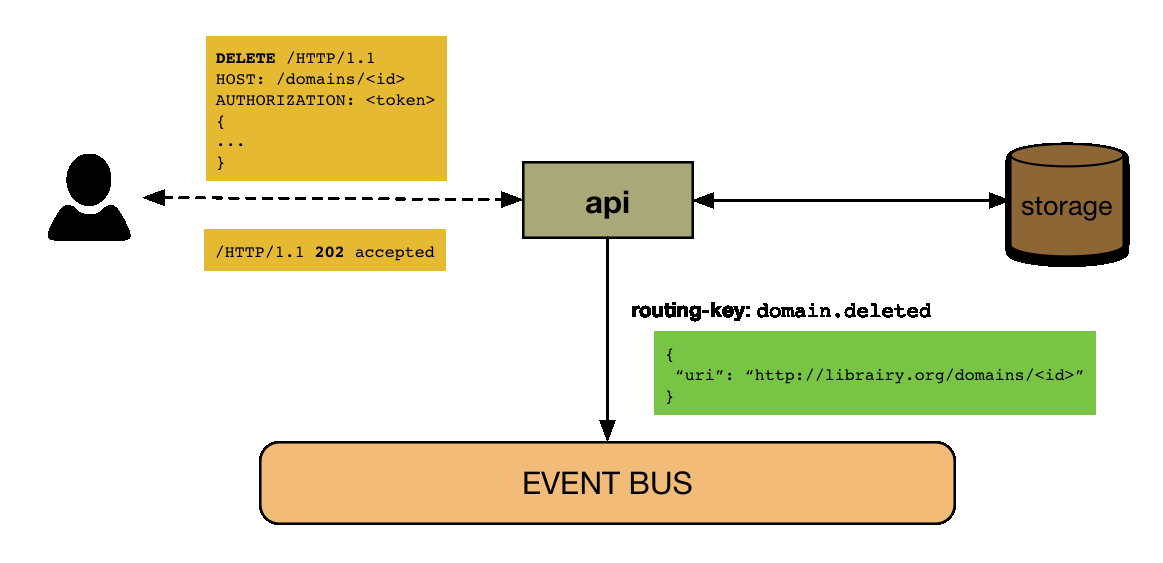
\includegraphics[scale=0.35]{api-domain-deleted}
  \caption{Domain deleted flow.}
  \label{fig:librairy-domain-deleted}
\end{figure}



\subsection{Event-driven Workflow}
Along with the resources mentioned above, there are two additional elements with an special participation in this system: \textit{modules} and \textit{events}. Both allow the workflow to be distributed. An event is a notification of new actions performed on resources. They are broadcasted so that any module is aware of the changes made to the resources. The modules are responsible for carrying out operations on the resources (e.g. text mining tools). They can perform actions on one or more resources in response to a new state reached by a given resource. Actions that can be paralleled by modules replicated through distributed environments.

The framework follows a publisher/subscriber approach where modules can publish and read \textit{events} to notify and to be notified about the state of a \textit{resource}. An event notifies a performed action (i.e. a resource and its new state), and follows the Representational State Transfer (REST)\cite{Fielding2002} paradigm. It contains the resource type and the new state reached by a specific resource ( i.e \textit{created}, \textit{deleted} or \textit{updated}). For example, when a new \textit{domain} is created, an \textit{event} message is published to the channel: $domain.created$. A channel is a space where events are published and modules are subscribed. Events on a channel can be managed by one or more modules, subscribed to that channel, that may perform an action (e.g. create a topic model when a domain have been created). Therefore, the workflow is not static and is not explicitly defined, instead distributed and emergent flows appear according to the modules subscribed to the event channels.

We use the Advanced Message Queuing Protocol (AMQP) as the messaging standard to avoid any cross-platform problem and any dependency to the selected message broker. This protocol defines: \textit{exchanges}, \textit{queues}, \textit{routing-keys} and \textit{binding-keys} to communicate publishers and consumers. A message sent by a publisher to an exchange is tagged with a routing-key. Consumers matching that routing-key with the binding-key used to link the queue to that exchange, will receive the message. This key follows the structure: \textit{resource.status}. Since a wildcard-based definition can be used to set the key, this paradigm allow modules both listening to individual type events (e.g. \'domains.created\' for new domains), or multiple type events (e.g. \#.created for all new resources).


\begin{figure}
  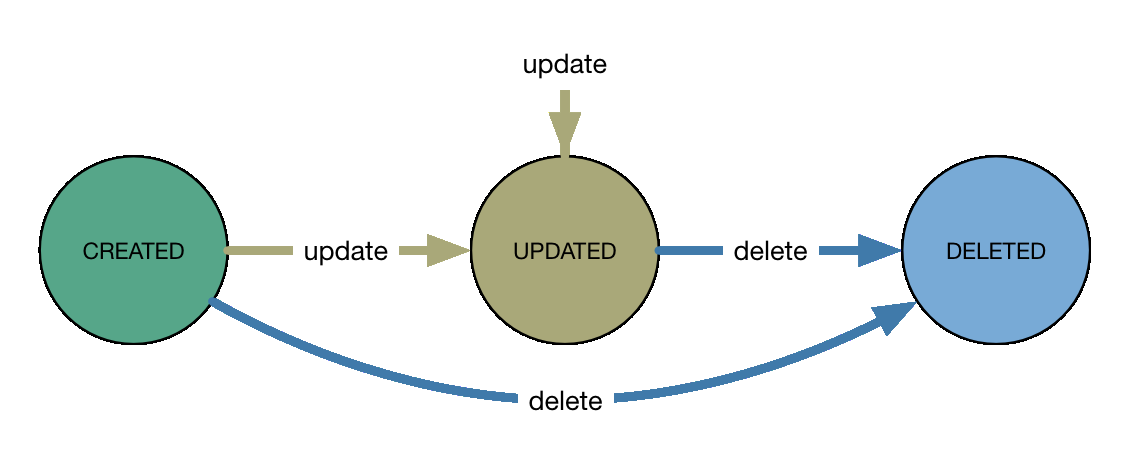
\includegraphics[scale=0.3]{resource-states}
  \caption{Resource states.}
  \label{fig:librairy-states}
\end{figure}

Each module is wrapped with a HTTP-Rest Application Program Interface (API) designed for interaction with end-users. Any external operation motivated by a user will be handled there. The 


Some of them, usually those related to reading operations, will be completely managed by this module getting all the data from the internal storage. However, those operations implying a modification of the status of some resource (e.g. creation of a \textit{document}), may be also performed by other modules listening for that type of event asynchronously. This module publishes to the following routing-keys: \textit{domain.(created;updated;deleted)}, \textit{document.(created;updated;deleted)}, \textit{part.(created;updated;deleted)}, and \textit{annotation.(created;updated;deleted)}.

\subsection{Working Modules}
A module is a processing unit that reacts to events generated from resources. They have been designed following the microservices architectural style. A module is a cohesive, since it implements only functionalities strongly related to the concern that it is meant to model \cite{Dragoni2016}, and independent process working on the framework with a specific purpose. This purpose is defined by both the routing-key and the binding-key associated to the events handled by the module. 

These are three main types of modules:
\begin{itemize}
	\item \textbf{Harvester}: creates resources such as \textit{documents}, \textit{parts-of} and \textit{domains}, from local or remote located textual files.
    \begin{itemize}[rightmargin=\dimexpr\linewidth-5cm-\leftmargin\relax]
    		\item Listening for: nothing
		\item Publishing to: \textit{document.(created)}, \textit{part.(created)}, \textit{domain.(created;updated)}
    \end{itemize}
    \item \textbf{Annotator}: retrieves named-entities, compounds, lemmas and makes annotations resulting of Natural Language Processing (NLP) task execution from \textit{documents} and \textit{parts}.
    \begin{itemize}[rightmargin=\dimexpr\linewidth-5cm-\leftmargin\relax]
    	\item Listening for: \textit{document.(created;updated)}, \textit{part.(created;updated)}
		\item Publishing to: \textit{annotation.(created;deleted)}
    \end{itemize}
    \item \textbf{Modeler}: builds representational models from a given \textit{domain}. 
    \begin{itemize}[rightmargin=\dimexpr\linewidth-5cm-\leftmargin\relax]
    	\item Listening for: \textit{domain.(created;updated)}
		\item Publishing to: \textit{annotation.(created;deleted)}
    \end{itemize}
\end{itemize}

\begin{figure}
  \includegraphics[scale=0.25]{modules}
  \caption{Modules.}
  \label{fig:librairy-modules}
\end{figure}



\section{Topic Model Service}
%present restful services to exploit a topic model
% topic-model-as-a-service

 


%\subsubsection{Storage}

%Multiple types of data can be handled in this ecosystem. Inspired in the Data Access Object (DAO) pattern, we have created a Unified Data Manager (UDM) providing access to any type of data used in the system.  Three types of databases have been considered:
%\begin{itemize}
	%\item \textbf{column-oriented database}: Focused on unique identified and/or \textit{structured data}. This storage allow %us searching key elements across resources. 
	%\item \textbf{document-oriented database}: Focused on indexing raw text. This storage allow us to execute advanced search %operations over all the information gathered about a textual resource. 
    %\item \textbf{graph database}: Focused on relations. This storage allow us exploring resources through the relationships %between them.
%\end{itemize}


\section{Summary}

A distributed framework is proposed where existing algorithms and tools coming from different technologies can work collaboratively to process and analyze huge collections of textual resources. This approach has been successfully applied to some real world scenarios \footnote{\url{http://drinventor.dia.fi.upm.es}}.
 
A new model definition based on the previously mentioned principle of maximizing information re-usability and minimize irrelevant data has been studied to create a fine-grained resource design. New domains, in the sense of particular vocabularies or specific textual formats, have been also analyzed to be included into the system via specific harvesters or more precise annotators. Moreover, a template-based mechanism oriented to facilitate the integration of new tools and techniques into the system has been built to make easier to develop new modules as well as increasing the available modules in public repositories.

% this file is called up by thesis.tex
% content in this file will be fed into the main document

%: ----------------------- introduction file header -----------------------
\chapter{Explainable Topic-based Associations}\label{ch:explainability}

\graphicspath{{explainability/figures/}}

% -------------------------------------------------------------
% -- Explainability
% -------------------------------------------------------------

As stated in Chapter \ref{ch:hypothesys}, one of our hypotheses aims to determine whether is possible to semantically relate texts from their most relevant topics (H1.2). In particular, our goal is to determine whether two documents can be related by identifying their most representative topics.

However, as seen in Section \ref{sec:topic-explainability}, interpreting how documents are related from their topic distributions is hard when using density-based measures. The same pair of documents may vary their distance from each other when using topic models with different dimensions to represent them, as shown in figure \ref{fig:topic_distances}. \textit{High dimensional models create more specific topics than models with fewer dimensions}, and this topic specificity influences the way in which topic distributions are related. 

In order to better understand the representivity of topics, in section \ref{sec:topic-relevance} we compare scientific articles from their topic distributions over different parts of texts. Two types of representativity are considered: (i) \textit{internal}, focused on describe the content, and \textit{external}, focused on discover relations.    

In Section \ref{sec:topic-clustering}, once we have identified the behavior of the topics to represent and relate texts from their distributions, we propose a new topic-based annotation based only on the most representative topics and a new distance measure that takes advantage of these representations. The main goal is not only to relate texts through their most relevant topics, but also to facilitate their interpretation. 


\section{Topic Relevance}
\label{sec:topic-relevance}


\section{Topic-based Clustering}
\label{sec:topic-clustering}


\section{Summary}

In Section \ref{sec:topic-relevance}, we have analyzed the representativeness of topics to describe texts. In the particular case of scientific articles, it is concluded that the abstracts are not sufficiently representative to describe, by means of topics, the content of a paper. This behavior suggests that texts with greater vocabulary that also emphasize key terms through repetition, favor topic-based representation.

Taking into account the relevance of topics to describe texts, we analyze in Section {\ref{sec:topic-clustering}} the behavior of topic distributions to calculate distances between documents using topic models with different dimensions. By using clustering techniques at the topic level, the most representative topics of a topic distribution are identified regardless of the number of dimensions that the model has. A topic-based representation is then proposed that covers the third research objective of this thesis (R03, \textit{define annotations based on topics that enable a semantic-aware exploration of the knowledge inside a corpus}). 

A new distance metric is also proposed that takes advantage of such representation to compare documents. Its performance is analyzed by automatically clustering the JRC-Acquis corpus according to EUROVOC categories. Tables XX and XY show results with high precision and recall in unsupervised classification tasks. This new way of relating documents from their most representative topics covers the fourth research objective of this thesis (R04, \textit{define a metric based on topic annotations that compares documents and facilitates their interpretation}). 

In order to perform the experiments, both the representation based on the most relevant topics and the distance metric based on these representations have been implemented in \textit{librAIry}. This partially covers the third and fourth technical objectives (T03, \textit{integrate the annotation method base on topic hierarchies into the topic model service}) (T04, \textit{create a system capable of finding similar document automatically}).

% this file is called up by thesis.tex
% content in this file will be fed into the main document

%: ----------------------- introduction file header -----------------------
\chapter{Large-scale Comparisons of Topic Distributions}\label{ch:comparisons}

\graphicspath{{comparisons/figures/}}

% -------------------------------------------------------------
% -- Comparisons
% -------------------------------------------------------------

\section{Document Similarity}

\section{Hashing Topic Distributions}

\section{Summary}

% this file is called up by thesis.tex
% content in this file will be fed into the main document

%: ----------------------- introduction file header -----------------------
\chapter{Cross-lingual Document Similarity}\label{ch:multilinguality}

\graphicspath{{multilinguality/figures/}}

% -------------------------------------------------------------
% -- Multilinguality
% -------------------------------------------------------------
% - Mimno et al., 2009. Polylingual topic models.
% - Jagarlamudi & Daume III, 2010. Extracting multilingual topics from unaligned comparable corpora.
% - Boyd-Graber & Resnik, 2010. Holistic sentiment analysis across languages: Multilingual supervised latent Dirichlet allocation.
% - Shi et al., 2016. Detecting common discussion topics across culture from news reader comments. 
% - Hao & Paul, 2018. Learning Multilingual Topics from Incomparable Corpora.
% - Yuan et al., 2018. Multilingual Anchoring: Interactive Topic Modeling and Alignment Across Languages.
% - Yang et al., 2019. A Multilingual Topic Model for Learning Weighted Topic Links Across Corpora with Low Comparability.


As stated in Chapter \ref{ch:hypothesis}, the last of our hypotheses aims to determine whether documents in different languages can be related without having to translate them, by using language agnostic concepts derived from their main topics (H1.4). In particular, our goal is to find abstractions that capture the content of documents, independently from the language used, in order to draw relations between them. 

A way to obtain this behaviour is by creating multilingual topics from comparable or parallel corpora, and relating documents from their topic distributions (See Section \ref{sec:multi-topic-alignment}) \citep{Graber2009, Boyd-Graber2010, Vulic2015}. A parallel corpora contains sentence-aligned documents (e.g. Europarl\footnote{https://ec.europa.eu/jrc/en/language-technologies/dcep} corpora) \citep{Steinberger2014}, and a comparable corpora contains theme-aligned documents (e.g. Wikipedia\footnote{https://www.wikipedia.org/} articles) \citep{Ni2009, Ni:2011:CLT:1935826.1935887}. Other types of abstractions may be obtained using multilingual dictionaries to translate documents in a common language from which they can be related \citep{errez2016, Liu2015a, Ma2017}. 


%Recent advances in machine translation techniques based on complex language models (BERT, GPT-3) could alleviate the requirement of multilingual training corpora by creating topic models from language-independent word representations (embeddings). But this approach loses the richness in describing topics, through their most representative words, that models have when created for each language independently. 

Recent advances in machine translation techniques based on the use of distributed representations of language \citep{Dabre2020ASO} could alleviate the requirement of multilingual training corpora by creating language-independent word representations. Unlike classical statistical approaches \citep{nakov-ng-2009-improved}, neural machine translation framework can naturally handle translation between more than one language pair \citep{ChenLiu2018, neubig-hu-2018-rapid}. These systems tend to generalize better due to exposure to diverse languages, leading to improved translation quality compared to bilingual systems. This particular phenomenon is known as translation knowledge transfer \citep{Pan2010} (i.e. “knowledge transfer” or “transfer learning”). However, the use of machine translation techniques to create topic spaces across languages may loses the richness in describing independently topics for each language through their most representative words. Similar topics in different languages do not necessarily correspond to the translation of their most representative words. For example, the topic 'economic development' created from EU legal regulations using English texts is described with the following top5 words\footnote{\url{http://librairy.linkeddata.es/jrc-en-model/topics/330/words}}: develop, strategy, growth, regional, international, reform; while when using Spanish texts its most representative words are\footnote{\url{http://librairy.linkeddata.es/jrc-es-model/topics/330/words}}: acción, financiación, alimentario, apoyo, compromiso. The words are not direct translations, but are used to refer to the same theme. These topic models are described further in section \ref{sec:crosslingual-models}. 

Modern language models make it possible to relate terms across languages based on word sequences. However, topic models assume bags of words and, therefore, the sequence of terms is unknown. Multilingual topics need to be related in order to be described independently by each language without compromising the ability to create unique representation spaces across languages. Approaches based on aligned corpora require prior knowledge at document-level (by parallel or comparable corpora) or at word-level (by dictionaries) to create topic models that represent documents in a common, language-independent space. In this way, the pre-established language relations condition the creation of the topics (supervised method), instead of being inferred from the topics themselves as a posteriori knowledge (non-supervised method). We propose a completely unsupervised way of building cross-lingual topic models based on sets of cognitive synonyms (\textit{synsets}) to discover relations between language-specific topics once the models (for each language) have been created. It does not require parallel or comparable data for training \citep{Badenes-Olmedo2019, Badenes-Olmedo2019b}. The cross-lingual topic models can be used for large-scale multilingual document classification and information retrieval tasks.

In Section \ref{sec:synset-space}, we propose conceptual abstractions for topic models. Topics are no longer described by words, but by language agnostic concepts. Cross-lingual topic models were created following this approach to describe documents from the most relevant concepts of their topics. The ability of these models to classify multilingual documents and to perform cross-lingual information retrieval were evaluated.

\section{Synset-based Representational Space}
\label{sec:synset-space}

In our approach, we propose annotating each topic with a list of synsets \citep{Bond2013} retrieved from WordNet\footnote{https://wordnet.princeton.edu/}\citep{Miller1995WordNet:English} based on its top $n$ words (Fig \ref{fig:density_hash2}). Word by word are queried in WordNet to retrieve its synsets. The final set of synsets for a topic is the union of the synsets from the individual top-words of a topics. Based on empirical evidence from different executions of the algorithm, n=5 is the configuration that offered the best performance in our tests. Let's look at an example to clarify how it works. Given the topics of Table \ref{tb:topics}, the EN-Topic (\textit{"communications systems"}) is annotated with the following synset list: \textit{radio.a.01, radio.v.01, radio.n.03, radio.n.01, radio\_receiver.n.01, equipment.n.01, network.n.02, network.n.04, network.v.01, network.n.05, network.n.01, net.n.06, communication.n.02, communication.n.03, communication.n.01, regulative.s.01}. The list of synsets for the ES-Topic (\textit{"sistema de comunicaci\'on"}) is:  \textit{kit.n.02,team.n.01, equipment.n.01, net.n.02, net.n.05, network.n.05, web.n.06, network.n.01, web.n.02, communication.n.02, communication.n.01, announcement.n.02, spectrum.n.02, spectrum.n.01, creep.n.01, ghost.n.01, apparition.n.02, electromagnetic.a.01}. And the list for FR-Topic (\textit{"systeme de communication"}) is:  \textit{access.n.02, approach.n.07, approach.n.02, access.n.06, access.n.03, access.n.05, assault.n.03, bout.n.02, approach.n.01, entree.n.02, entry.n.01, entrance.n.01, entry.n.03, admission.n.01, submission.n.01, introduction.n.01}. The librAIry NLP service\footnote{http://librairy.linkeddata.es/nlp} was used to identify the list of synsets from a topic description based on top words. It is based on the Open Multilingual WordNet\footnote{http://compling.hss.ntu.edu.sg/omw/} \citep{Bond2012}.

\subsection{Document representation}
Documents (i.e seen as data points in the generated topic-based space) are transformed from the original feature space based on mono-lingual topic distributions into a hierarchical-code space, so that similar data points share relevant cross-lingual concepts. Since topic models create latent themes from word co-occurrence statistics in a corpus, a cross-lingual concept specifies the knowledge about the word-word relations it contains for each language. This abstraction can be extended to cover the knowledge derived from sets of topics. The topics are obtained via LDA and hierarchically divided into groups with different degrees of semantic specificity in a document (See Chapter \ref{ch:comparisons}). Documents represented as a weighted mixture of latent topics (per-document topic distributions) are then annotated in these feature spaces with the relation between topics inside each hierarchy level. Regardless of their language, they are then described by cross-lingual concepts (based on WordNet-synset annotations) and hash codes are calculated to summarize their content. The hash expression sets a 3-level hierarchy of cross-lingual concepts. Topics with similar presence in a document (i.e. relevance) are grouped together in the same hierarchical level (Fig \ref{fig:density_hash2}) similarly to what was presented in section \ref{sec:comparison-experiments}. Each level of the hierarchy indicates the importance of the topic according to its distribution. \textit{Level 0} describes the topics with the highest score. \textit{Level 1} describes the topics with highest score once the first ones have been eliminated, and so on. Documents are described by vectors containing set of topics (i.e. set of synsets), where each dimension means a topic relevance. Given a document $d$ with a topic distribution $q = [t0=0.28, t1=0.05, t2=0.44, t3=0.23]$, the hash expression may be $H_d = {(ts2), (ts0,ts3), (ts1)}$. It means that topic $t2$ described by the synset $ts2$ is the most relevant (i.e 0.44 score), then topics $t0$ and $t3$ described by synsets $ts0$ and $ts3$ (i.e 0.28 and 0.23 scores) and, finally, topic $t1$ described by synset $ts1$ (i.e 0.05).

\begin{figure}[!htbp]\centering
\includegraphics[scale=0.35]{density-hash.png}
\caption{Cross-lingual hash-expression (H) of a document based on WordNet-synset annotations created from the top words of each topic distribution. The most relevant topics are grouped according to their importance in three levels (h0, h1 and h2)}
\label{fig:density_hash2}
\end{figure}


\subsection{Similarity metric}
\label{sec:cl-sim-metric}
In this workspace based on hierarchical representations of topics we use the distance metric proposed in Section \ref{sec:large-distance-metric}, based on the Jaccard coefficient. This metric is mainly used for set-type data \citep{Li2012, Ji2013, Li2010b, Zhao2013} and computes the similarity of sets by looking at the relative size of their intersection (See Eq. \ref{eq:jc}). Thus, it allows us to measure the intersection of cross-lingual topics described by hierarchical hash-sets:

%distance metric formula
\begin{equation}
d_H(H_A,H_B) = \sum\limits_{l=1}^L \Big( d_J(H_A(h_l),H_B(h_l)) \Big) = 
\sum\limits_{l=1}^L \Big( 1 - \frac{H_A(h_l) \cap H_B(h_l)}{H_A(h_l) \cup H_B(h_l)} \Big) 
\label{eq:dh2}
\end{equation}

where $H_A$ and $H_B$ are hash codes, $H_A(h_l)$ and $H_B(h_l)$ are the set of topics up to level $l$ for each hash code $H$,  and $L$ is the maximum hierarchy level. A corner case is $L=T$, where $T$ is the number of topics in the model. 

\subsection{Cross-lingual Models}
\label{sec:crosslingual-models}

\begin{figure*}[ht]\centering
\includegraphics[scale=0.4]{latent-topic-models.png}
\caption{Graphical representation of the model that relies on the latent layer of cross-lingual topics obtained by LDA and hash functions through hierarchies of synsets. Mono-lingual approaches force to translate the documents to the same language to represent them in a unique feature space. Multi-language approaches require previously aligned topics from different languages so that documents can be represented in an equivalent feature space. Cross-lingual Synset-based approach creates a new space by combining the feature spaces of each language (i.e synsets from topn topic words). Documents are then represented in this unique space.}
\label{fig:cross-lingual_topics}
\end{figure*}

Our approach considers that cross-lingual models can be built from non-parallel or even non-comparable collections of multilingual documents. It first creates a probabilistic topic model for each language separately, and then annotates the topics with cross-lingual labels (Fig \ref{fig:cross-lingual_topics}). In the same way, the topic distribution of documents expressed through weighted vectors are first transformed into hierarchies of topics according to their relevance. And then documents are described by a 3-level hierarchy of cross-lingual concepts.

In order to be able to compare the performance of our unsupervised algorithm with a semi-supervised algorithm (MuPTM-based) it is necessary to use theme-aligned corpora that map topics across languages. We used the JRC-Acquis\footnote{https://ec.europa.eu/jrc/en/language-technologies/jrc-acquis} corpora \citep{Steinberger2006}. It is a collection of legislative texts written in 23 languages, although we only use English, Spanish,  French, Italian and Portuguese editions for the tests. Most texts have been manually classified into subject domains according to the EUROVOC\footnote{http://eurovoc.europa.eu/} thesaurus \citep{Eurovoc1995}, which exists in one-to-one translations into approximately twenty languages and distinguishes about 6,000 hierarchically organised descriptors (subject domains). More than 20k documents were used for each language-specific model, a total of 112,569 texts are included in the training-test package, which is publicly available\footnote{http://librairy.linkeddata.es/data/jrc/select?q=*:*} for reuse.

The JRC-Acquis corpus is annotated with EUROVOC categories. These categories are shared among languages and will serve as support for building the topic models. Moreover, the topic independence assumption \citep{Blei2003} of LDA models should be also satisfied, so the categories must first be moved to their base concepts and therefore disjointed categories. The EUROVOC taxonomy has 7,193 concepts/labels from 21 domain areas such as politics, international relations, european union, law, economics, etc. There are 4,904 reciprocal hierarchical relationships (no polyhierarchy) and 6,992 reciprocal associative relationships. Using hierarchical relations, we identified the root concepts from which all other categories derive. The initial 7,193 labels were then reduced to 452 labels, which are independent (topic independence assumption from LDA is satisfied), and can be used to train the topic models. 

\begin{table*}[ht]\centering
  \small
  \noindent
  \begin{tabularx}{\linewidth}{@{} CCCCC @{}}
  \hline
 \textbf{EN-Topic 3} & \textbf{ES-Topic 3} & \textbf{FR-Topic 26} & \textbf{PT-Topic 10} & \textbf{IT-Topic 3}  \\
\textbf{\textit{{\scriptsize "communications systems"}}} & \textbf{\textit{{\scriptsize "sistema de comunicaci\'on"}}} & \textbf{\textit{{\scriptsize "systeme de communication"}}} & \textbf{\textit{{\scriptsize "meios de comunicação"}}} & \textbf{\textit{{\scriptsize "strutture di comunicazione"}}} \\ 
  \hline
     radio          & equipo                & communications		& rede         & rete        \\
     equipment      & red                   & reseaux            & comunicação   & comunicazione        \\
     network        & comunicaci\'on        & electroniques      & electronico    & apparecchiatura        \\
     communication  & espectro              & acces              & acesso    & radio        \\
     regulatory     & electromagn\'etico    & telecommunications & utilizador & regolamentazione            \\
     spectrum       & electr\'onico         & service            & operador & spettro           \\
     electronic     & reglamentaci\'on      & universel          & regulador    & elettronico                  \\
     access         & banda                 & reglamentaires     & universal        & armonizzare        \\
     standard       & etsir                 & nationales         & garantir   & mobile         \\
     mobile         & compatibilidad        & fourniture         & regulamentar  & banda          \\
    \bottomrule
  \end{tabularx}
\caption{Randonly selected theme-aligned topics described by top 10 words based on EUROVOC annotations from JRC-Acquis dataset}
\label{tb:topics}
\end{table*}

 A pre-processing of the documents was required to clean texts and to build a suitable data set for the model. Terms with high frequency are assumed not specific to a particular topic, so words present in more than 90\% of the corpus are considered stopwords and removed from the model. Also, rare terms that occur infrequently are considered not representative of a single topic since they do not appear enough to infer that it is salient for a topic. Then, words present in less than 0.5\% of the corpus are also removed from the model. Lemmatized expressions of names, verbs and adjectives were used to create the bag-of-words, and documents with less than 100 characters were discarded since LDA has proven to have lower performance with these type of texts \citep{Cheng2014a}. 
 
 Then, we set the number of topics $K=500$ (several configurations were evaluated, but this was the closest to the performance obtained with the supervised model based on categories). We run the Gibbs samplers for 1000 training iterations on LDA from our librAIry framework. The Dirichlet priors $\alpha=0.1$ and $\beta=0.01$ were set following \citep{Hu2014a}. Once the word distributions for each topic is available, the list of synsets related with the top5 words for each topic are identified (this number is set to offer better performance after trying several alternatives). Finally, the 3-level hierarchy of topics per document is replaced by a 3-level hierarchy of synsets. Probabilistic topic models in Spanish\footnote{http://librairy.linkeddata.es/jrc-es-model-unsupervised}, English \footnote{http://librairy.linkeddata.es/jrc-en-model-unsupervised}, French\footnote{http://librairy.linkeddata.es/jrc-fr-model-unsupervised}, Italian\footnote{http://librairy.linkeddata.es/jrc-it-model-unsupervised} and Portuguese\footnote{http://librairy.linkeddata.es/jrc-pt-model-unsupervised} were created independently without previously establishing any type of alignment between their topics.
 
 In order to compare the performance of this non-supervised approach with approaches based on aligned topics, we need to use a variant of LDA to force the correspondence between the 452 root categories identified in the EUROVOC thesaurus and the latent topics of the model. Thus, LabeledLDA \citep{Ramage2009a}, a supervised version of LDA, was used to perform parameter estimation. Theme-aligned probabilistic topic models in Spanish\footnote{http://librairy.linkeddata.es/jrc-es-model}, English \footnote{http://librairy.linkeddata.es/jrc-en-model}, French\footnote{http://librairy.linkeddata.es/jrc-fr-model}, Italian \footnote{http://librairy.linkeddata.es/jrc-it-model} and Portuguese \footnote{http://librairy.linkeddata.es/jrc-pt-model} were created sharing the topics but not its definitions (i.e. vocabulary) (see table \ref{tb:topics}).

A simple way of looking at the output quality of the topic models is by simply inspecting top words associated with a particular topic learned during training. A latent topic is semantically coherent if it assigns high probability scores to words that are semantically related \citep{Gliozzo2007, newman-etal-2010-automatic, mimno-etal-2011-optimizing}. It is much easier for humans to judge semantic coherence of cross-lingual topics and their alignment across languages when observing the actual words constituting a topic. These words provide a shallow qualitative representation of the latent topic space, and could be seen as direct and comprehensive word-based summaries of a large document collection.

Samples of cross-lingual topics are provided in Table \ref{tb:topics}. We may consider this visual inspection of the top words associated with each topic as an initial qualitative evaluation, suitable for human judges. Documents present similar topic distributions when projecting their content on topics according to their language as can be seen in fig \ref{fig:topic_distributions}. Since the topic identifiers are not aligned, the graphs appear displaced.

\begin{figure}[ht]\centering
\includegraphics[scale=0.4]{topic-dist.png}
\caption{topic distributions from the same document in English ($h_{EN}=\{(t3062),(t335),(t8278)\}$) and Spanish ($h_{ES}=\{(t335),(t4060),(t5769)\}$).}
\label{fig:topic_distributions}
\end{figure}



\section{Evaluation}
\label{sec:crosslingual-evaluation}

A way to evaluate our cross-lingual document similarity algorithm is to test how well it performs in practice for different real-life tasks: document classification and information retrieval. Evaluation is done using the B-Cubed metrics \citep{Bagga1998} to estimate the fit between two clusters, the one obtained from a supervised category-based topic alignment algorithm and the one obtained from our unsupervised synset-based topic alignment algorithm. 

% table monolingual JRC
\begin{table}[ht]\centering
\begin{center}
\small
\begin{tabular}{cc|rr||rr||rr||rr||rr}
    \hline
    \multicolumn{12}{c}{\textbf{JRC-Acquis Corpora}} \\
    \hline
    & & \multicolumn{2}{c}{\textbf{en}} &
      \multicolumn{2}{c}{\textbf{es}} &
      \multicolumn{2}{c}{\textbf{fr}} &
      \multicolumn{2}{c}{\textbf{pt}} &
      \multicolumn{2}{c}{\textbf{it}}\\
    & & {\textit{cat}} & {\textit{syn}} & {\textit{cat}} & {\textit{syn}} & {\textit{cat}} & {\textit{syn}} & {\textit{cat}} & {\textit{syn}} & {\textit{cat}} & {\textit{syn}} \\
    \hline
    \multirow{4}{*}{\textbf{prec}} 
    &{\textit{min}}     &0.01 &0.01 &0.01 &0.01 &0.01 &0.01 &0.01 &0.01 &0.01 &0.01 \\
    &{\textit{max}}     &1.00 &0.95 &1.00 &0.87 &1.00 &0.87 &1.00 &0.83 &1.00 &0.85\\
    &{\textit{mean}}    &\textbf{0.58} &0.48 &\textbf{0.55} &0.48 &\textbf{0.55} &0.41 &\textbf{0.53} &0.42 &\textbf{0.54} &0.45 \\
    &{\textit{dev}}     &0.27 &0.23 &0.27 &0.22 &0.26 &0.20 &0.24 &0.21 &0.25 &0.22 \\
    \hline
    \multirow{4}{*}{\textbf{rec}} 
    &{\textit{min}}     &0.01 &0.03 &0.01 &0.04 &0.01 &0.05 &0.01 &0.04 &0.01 &0.05\\
    &{\textit{max}}     &0.96 &1.00 &0.93 &1.00 &0.95 &1.00 &0.92 &1.00 &0.94 &1.00\\
    &{\textit{mean}}    &0.39 &\textbf{0.52} &0.36 &\textbf{0.49} &0.42 &\textbf{0.51} &0.40 &\textbf{0.47} &0.39 &\textbf{0.48} \\
    &{\textit{dev}}     &0.24 &0.20 &0.23 &0.20 &0.23 &0.23 &0.23 &0.21 &0.23 &0.20 \\
    \hline
    \multirow{4}{*}{\textbf{f1}} 
    &{\textit{min}}     &0.02 &0.03 &0.01 &0.02 &0.02 &0.03 &0.02 &0.02 &0.01 &0.02 \\
    &{\textit{max}}     &0.70 &0.75 &0.70 &0.71 &0.70 &0.73 &0.70 &0.71 &0.70 &0.72\\
    &{\textit{mean}}    &0.35 &\textbf{0.42} &0.32 &\textbf{0.41} &0.37 &\textbf{0.39} &0.35 &\textbf{0.38} &0.31 &\textbf{0.40} \\
    &{\textit{dev}}     &0.16 &0.15 &0.15 &0.15 &0.17 &0.17 &0.16 &0.16 &0.16 &0.15\\
\end{tabular}
\end{center}
\caption{Document classification performance (precision-'prec', recall-'rec' and fMeasure-'f1') of the categories-based (\textit{cat}) and synset-based (\textit{syn}) topic alignment algorithms in monolingual document collections}
\label{tb:mono-class}
\end{table}


Let $CL_i$ be the cluster that document $t_i$ gets clustered in, and $G_i$ its correct cluster from the ground truth. The B-Cubed metric then calculates $precision=\frac{|CL_i \cap G_i|}{|CL_i|}$ and $recall=\frac{|CL_i \cap G_i|}{|G_i|}$. The total precision and recall of the clustering are taken as the average of the precision and recall scores over all documents. Results are also presented in terms of the $F_1$ measure to balance between precision and recall: $F_1=\frac{2 \cdot precision \cdot recall}{precision + recall}$. The aim is to measure the performance of the algorithm taking into account documents with manual category assignments.

\subsection{Cross-lingual Document Classification}
\label{sec:cl-doc-class}
A random group of 1k documents from the JRC-Acquis corpora, which have not been used to train the models, is considered for evaluation as they are manually tagged with EUROVOC categories. For each document, the cluster to which it belongs is identified from its categories. This cluster is then compared (B-Cubed metrics) with the one obtained from the labels generated from its most representative topics (\textit{cat}) and with the one obtained from the labels generated with the WordNet-Synsets of those topics (\textit{syn}). Algorithm performance is evaluated in monolingual, bilingual, and multilingual document collections (tables \ref{tb:mono-class} and \ref{tb:multi-class} ) .

% table multi-lingual JRC
\begin{table}[ht]\centering
\begin{center}
\small
\begin{tabular}{cc|rr||rr||rr||rr}
    \hline
    \multicolumn{10}{c}{\textbf{JRC-Acquis Corpora}} \\
    \hline
    & & \multicolumn{2}{c}{\textbf{en-es}} &
      \multicolumn{2}{c}{\textbf{en-es-fr}} &
      \multicolumn{2}{c}{\textbf{en-es-fr-pt}} &
      \multicolumn{2}{c}{\textbf{en-es-fr-pt-it}} \\
    & & {\textit{cat}} & {\textit{syn}} & {\textit{cat}} & {\textit{syn}} & {\textit{cat}} & {\textit{syn}} & {\textit{cat}} & {\textit{syn}} \\
    \hline
    \multirow{4}{*}{\textbf{prec}} 
    &{\textit{min}}     &0.01 &0.01 &0.01 &0.01 &0.01 &0.01 &0.01 &0.01\\
    &{\textit{max}}     &1.00 &0.97 &1.00 &0.98 &1.00 &0.97 &1.00 &0.98\\
    &{\textit{mean}}    &\textbf{0.62} &0.55 &\textbf{0.59} &0.52 &\textbf{0.56} &0.50 &\textbf{0.57} &0.52\\
    &{\textit{dev}}     &0.26 &0.23 &0.26 &0.25 &0.26 &0.26 &0.26 &0.26\\
    \hline
    \multirow{4}{*}{\textbf{rec}} 
    &{\textit{min}}     &0.01 &0.09 &0.01 &0.07 &0.01 &0.06 &0.01 &0.04\\
    &{\textit{max}}     &1.00 &1.00 &0.86 &0.93 &0.83 &0.91 &0.80 &0.89\\
    &{\textit{mean}}    &0.33 &\textbf{0.57} &0.25 &\textbf{0.39} &0.21 &\textbf{0.36} &0.23 &\textbf{0.37}\\
    &{\textit{dev}}     &0.16 &0.23 &0.13 &0.15 &0.12 &0.13 &0.12 &0.15\\
    \hline
    \multirow{4}{*}{\textbf{f1}} 
    &{\textit{min}}     &0.02 &0.02 &0.02 &0.05 &0.02 &0.06 &0.02 &0.08\\
    &{\textit{max}}     &0.75 &0.81 &0.62 &0.66 &0.61 &0.64 &0.59 &0.62\\
    &{\textit{mean}}    &0.36 &\textbf{0.49} &0.30 &\textbf{0.38} &0.29 &\textbf{0.35} &0.30 &\textbf{0.36}\\
    &{\textit{dev}}     &0.16 &0.18 &0.11 &0.12 &0.11 &0.11 &0.11 &0.12\\
\end{tabular}
\end{center}
\caption{Document classification performance (precision-'prec', recall-'rec' and fMeasure-'f1') of the categories-based (\textit{cat}) and synset-based (\textit{syn}) topic alignment algorithms in multi-lingual document collections}
\label{tb:multi-class}
\end{table}

The results show a higher performance of the semi-supervised algorithm (categories-based topic alignment) in terms of precision, and of the unsupervised algorithm (synset-based topic alignment) in terms of coverage. The cause lies in the set of synonyms generated by WordNet, being able to share the same synset for two different topics. From a more general point of view (fMeasure), the benefit obtained by the increase in coverage (recall) is greater than by the loss of accuracy (precision).


\subsection{Cross-lingual Information Retrieval}
\label{sec:cl-inf-retrieval}
Given a set of documents and a text, the task is to rank the documents according to their relevance to the query text regardless of the language used. The JRC-Acquis corpus is used because by having texts tagged with EUROVOC categories we can build a ground-truth set grouping the documents that share the same codes as those used in the query document. A collection of 1k randomly selected documents (monolingual, bi-lingual and multi-lingual) are annotated by the category-based and synset-based topic alignment algorithms. Then, we randomly take articles to search in D for documents that share the same categories than the query document (i.e  the ground-truth set). Next, the query text is used to search in D for similar documents using category-based annotations and synset-based annotations. We evaluate the performance of the algorithms in terms of precision@3, precision@5 and precision@10 (tables \ref{tb:mono-ir} and \ref{tb:multi-ir} ) .

% table monolingual TED
\begin{table}[ht]\centering
\begin{center}
\small
\begin{tabular}{cc|rr||rr||rr||rr||rr}
    \hline
    \multicolumn{12}{c}{\textbf{JRC-Acquis Corpora}} \\
    \hline
    & & \multicolumn{2}{c}{\textbf{en}} &
      \multicolumn{2}{c}{\textbf{es}} &
      \multicolumn{2}{c}{\textbf{fr}} &
      \multicolumn{2}{c}{\textbf{pt}} &
      \multicolumn{2}{c}{\textbf{it}} \\
    & & {\textit{cat}} & {\textit{syn}} & {\textit{cat}} & {\textit{syn}} & {\textit{cat}} & {\textit{syn}} & {\textit{cat}} & {\textit{syn}} & {\textit{cat}} & {\textit{syn}} \\
    \hline
    \multirow{2}{*}{\textbf{p@3}} 
    &{\textit{mean}}    &\textbf{0.84} &0.83 &\textbf{0.81} &0.78 &\textbf{0.83} &0.74 &\textbf{0.79} &0.78 &\textbf{0.80} &0.75 \\
    &{\textit{dev}}     &0.26 &0.26 &0.27 &0.29 &0.26 &0.32 &0.27 &0.29 &0.27 &0.29 \\
    \hline
    \multirow{2}{*}{\textbf{p@5}} 
    &{\textit{mean}}    &\textbf{0.82} &0.80 &\textbf{0.79} &0.75 &\textbf{0.80} &0.72 &\textbf{0.77} &0.75 &\textbf{0.78} &0.72 \\
    &{\textit{dev}}     &0.25 &0.25 &0.25 &0.27 &0.25 &0.29 &0.25 &0.26 &0.26 &0.28 \\
    \hline
    \multirow{2}{*}{\textbf{p@10}} 
    &{\textit{mean}}    &\textbf{0.77} &0.76 &\textbf{0.75} &0.73 &\textbf{0.77} &0.68 &\textbf{0.72} &0.71 &\textbf{0.74} &0.68 \\
    &{\textit{dev}}     &0.23 &0.25 &0.25 &0.27 &0.24 &0.27 &0.25 &0.27 &0.25 &0.26 \\
\end{tabular}
\end{center}
\caption{Information retrieval performance (precision@3, precision@5 and precision@10) of the categories-based (\textit{cat}) and synset-based (\textit{syn}) topic alignment algorithms in monolingual document collections}
\label{tb:mono-ir}
\end{table}

% table multi-lingual TED
\begin{table}[ht]\centering
\begin{center}
\small
\begin{tabular}{cc|rr||rr||rr||rr}
    \hline
    \multicolumn{10}{c}{\textbf{JRC-Acquis Corpora}} \\
    \hline
    & & \multicolumn{2}{c}{\textbf{en-es}} &
      \multicolumn{2}{c}{\textbf{en-es-fr}} &
      \multicolumn{2}{c}{\textbf{en-es-fr-pt}} &
      \multicolumn{2}{c}{\textbf{en-es-fr-pt-it}} \\
    & & {\textit{cat}} & {\textit{syn}} & {\textit{cat}} & {\textit{syn}} & {\textit{cat}} & {\textit{syn}} & {\textit{cat}} & {\textit{syn}} \\
    \hline
    \multirow{2}{*}{\textbf{p@3}} 
    &{\textit{mean}}    &\textbf{0.84} &0.79 &\textbf{0.85} &0.75 &\textbf{0.81} &0.69 &\textbf{0.82} &0.71\\
    &{\textit{dev}}     &0.25 &0.28 &0.24 &0.31 &0.23 &0.29 &0.25 &0.29\\
    \hline
    \multirow{2}{*}{\textbf{p@5}} 
    &{\textit{mean}}    &\textbf{0.82} &0.76 &\textbf{0.81} &0.72 &\textbf{0.78} &0.67 &\textbf{0.79} &0.69\\
    &{\textit{dev}}     &0.24 &0.26 &0.23 &0.27 &0.24 &0.25 &0.21 &0.26\\
    \hline
    \multirow{2}{*}{\textbf{p@10}} 
    &{\textit{mean}}    &\textbf{0.78} &0.73 &\textbf{0.76} &0.67 &\textbf{0.73} &0.62 &\textbf{0.74} &0.63\\
    &{\textit{dev}}     &0.22 &0.24 &0.23 &0.26 &0.22 &0.24 &0.23 &0.24\\
\end{tabular}
\end{center}
\caption{Information retrieval performance (precision@3, precision@5 and precision@10) of the categories-based (\textit{cat}) and synset-based (\textit{syn}) topic alignment algorithms in multi-lingual document collections}
\label{tb:multi-ir}
\end{table}

Although the precision values are lower than those obtained by semi-supervised approximation, they are sufficiently promising (around 0.75) to think that introducing improvements in the lemmatization process would increase the quality of the WordNet-synset annotations derived from the most representative words of each topic (precision values close to 0.8 in the English corpus).

\subsection{Text Length on Cross-lingual Representations}

The ability of topics to materialize the underlying knowledge of the documents depend on the texts used to train models. We have studied the impact that the length of texts has, since they determine the space where words can co-occur, to semantically relate multilingual documents described in a probabilistic topic space and, therefore, to capture the knowledge derived from their relationships \citep{Lozano2020}. 

The aim is to know how text length influences the cross-lingual topics created to semantically relate multilingual documents through state-of-the-art similarity metrics (See Chapter \ref{ch:soa}). We have designed several document retrieval tasks based on the models described in Section \ref{sec:crosslingual-models}, to compare the clusters of documents created from their manual annotations (i.e. EUROVOC tags) with those created automatically from their topic distributions (Fig.\ref{fig:workflow}). 

\begin{figure}[ht]
    \centering
    \includegraphics[width=1.0\linewidth]{workflow.png}
    \caption{Preparation of experiments by creating topic models for each \\subset of the original corpus and cross-validated with EuroVoc thesaurus}
    \label{fig:workflow}
\end{figure}


The JRC-Acquis dataset used in the previous experiments (Section \ref{sec:cl-doc-class} and \ref{sec:cl-inf-retrieval}), was extended with the DGT-Acquis \citep{Steinberger2014} collection to increase the total number of documents and the diversity of text length. It contains documents from the Official Journal of the European Union from 2004 to 2011. Given that both datasets are constructed from the same domain with no overlap for data since 2007, we decided to merge both of them into a single collection, the Acquis corpus, formed with all the JRC-Acquis dataset and the documents of DGT-Acquis from that year. \textit{English} and \textit{Spanish} versions of the Acquis corpus were used to validate the results across languages (see table \ref{table:acquis_summ} for a summary of the data used). 

\begin{table}[ht]
\centering
\begin{adjustbox}{max width=0.9\textwidth}
\begin{tabular}{cc|ccc|ccc}
\cline{3-8}
                           &          & \multicolumn{3}{c|}{English}        & \multicolumn{3}{c}{Spanish}         \\ \cline{3-8} 
                           &          & DGT      & JRC      & Acquis   & DGT      & JRC      & Acquis   \\ \hline
\multicolumn{2}{c|}{Documents}      & 51521    & 16260    & 67781    & 51585    & 16470    & 68055    \\ \hline
\multirow{5}{*}{Tokens} & Median   & 135      & 197      & 152      & 129      & 204      & 150      \\
                           & Mean     & 185.8762 & 261.9931 & 204.1359 & 181.9172 & 271.2842 & 203.5449 \\
                           & Variance & 34806.26 & 35716.91 & 36080.66 & 34624.02 & 38700.03 & 37074.97 \\
                           & Min      & 7        & 7        & 7        & 6        & 6        & 6        \\
                           & Max      & 1360     & 1063     & 1360     & 1411     & 1110     & 1411     \\ \hline
\end{tabular}%
\end{adjustbox}
\vspace*{3mm}
\caption{Number of documents and tokens by dataset}
\label{table:acquis_summ}

\end{table}


Texts were pre-processed before the models were trained. We removed stopwords, including general NLP and domain-specific ones based on topic distributions. Rare terms with extremely low total document frequency were also removed. Words were lemmatized and changed to lower-case. A lower and an upper limit on the number of words (i.e. tokens) were defined to discard texts. These bounds were inferred from the interquartile range (Fig. \ref{fig:sizebox}). 


\begin{figure}[ht]\centering
   \begin{minipage}{0.49\textwidth}
     \frame{\includegraphics[width=\linewidth]{PreClean.png}}
     \caption{Before pre-processing}\label{subfig:preClean}
   \end{minipage}
   \begin {minipage}[c]{0.49\textwidth}
     \frame{\includegraphics[width=\linewidth]{cleaned.png}}
     \caption{After pre-processing}\label{subfig:postClean}
   \end{minipage}
   \caption{Distribution of articles by number of tokens in corpora}
   \label{fig:sizebox}
\end{figure}


We then divided the original corpora into several subsets (3, 6 and 9) of the same size with texts of similar length. The aim is to compare how similarity metrics based on topic distributions behave for each dataset in document retrieval tasks and to understand the influence of text lengths in the quality of multilingual topic models. For each data set, we reserved a sample ($5\%$) for testing and the rest ($95\%$) was used to train a topic model. The test set was projected in the topic space according to the trained model and then the similarity metrics were used to compare those documents with all documents in the corpus and obtain the most similar ones. The list with the top10 most similar documents is compared in terms of Mean Average Precision (MAP) with the one obtained when comparing them from the EuroVoc labels. This metric allows evaluating on average how good the first 10 results of a query are by taking the mean of all average precision for the first 10 results when comparing a list of retrieved documents and the ground truth.

Each document was manually annotated with one or more EuroVoc categories. Documents that share the same categories were therefore considered semantically related. For each document in the test set, its topic-based similarity to the others is calculated according to density-based metrics (\ref{sec:related-work}) such as Jensen-Shannon divergence (JSD) and Hellinger distance (HE); and our hierarchy-based metric (\ref{sec:large-distance-metric}) that we named Weighted Jaccard Levels (WJL) in experiments. The list of related documents from the EuroVoc categories is then compared to the list of related documents by topics expressed by density or by hierarchies. Since several topic models have been created for each dataset (with 50,100,300 and 500 topics), the precision results for each model were averaged following the mean average precision (MAP) metric. Thus, results reflect the capacity of each topic model to express the knowledge required to relate texts from their content without supervision. Table \ref{table:acquis} shows results for each trained model and each similarity metric. A distinction is made between texts written in English and Spanish. 


\begin{table}[ht]
\centering
\resizebox{0.6\textwidth}{!}{%
\begin{tabular}{ccccc}
\multicolumn{5}{c}{Acquis (MAP@10)}                                                                                                                           \\ \hline
\multicolumn{1}{c|}{Lang}                     & \multicolumn{1}{c|}{Topics} & JSD                               & HE      & WJL                               \\ \hline
\multicolumn{1}{c|}{\multirow{4}{*}{Spanish}} & \multicolumn{1}{c|}{50}     & \textbf{0.80060} & 0.79665 & 0.70583                           \\
\multicolumn{1}{c|}{}                         & \multicolumn{1}{c|}{100}    & \textbf{0.82741} & 0.77930 & 0.75555                           \\
\multicolumn{1}{c|}{}                         & \multicolumn{1}{c|}{300}    & \textbf{0.84261} & 0.58531 & 0.79036                           \\
\multicolumn{1}{c|}{}                         & \multicolumn{1}{c|}{500}    & \textbf{0.81238} & 0.68482 & 0.79336                           \\ \hline
\multicolumn{1}{c|}{\multirow{4}{*}{English}} & \multicolumn{1}{c|}{50}     & \textbf{0.81421} & 0.80150 & 0.73367                           \\
\multicolumn{1}{c|}{}                         & \multicolumn{1}{c|}{100}    & \textbf{0.85510} & 0.74060 & 0.80315                           \\
\multicolumn{1}{c|}{}                         & \multicolumn{1}{c|}{300}    & \textbf{0.84005} & 0.52082 & 0.83277                           \\
\multicolumn{1}{c|}{}                         & \multicolumn{1}{c|}{500}    & 0.78874                           & 0.43636 & \textbf{0.84555} \\ \hline \hline
\end{tabular}%
}
\vspace*{3mm}
\caption{Aggregated MAP results by metric and model}
\label{table:acquis}
\end{table}

The results suggest that PTM highly capture the knowledge required to relate semantically documents, since all models tested had at least one metric above 0.8 in precision. Among the metrics used to relate documents, the Jensen-Shannon divergence (JSD) offers a better performance in general terms compared to the other approaches. Although a downward trend is suggested in density-based metrics when increasing the number of topics, compared to hierarchical metrics that improve their performance when increasing the number of topics. This happens because the sum of distances of the less representative topics for JSD gets bigger as the number of topics diverge from its optimum while activated topics (i.e selected topics at one of the hierarchy levels) get more discriminative which lead to an increase of WJL. Another way to think about the number of topics is the level of detail they capture. Models with low number of topics will present general themes shared by all documents. On the contrary, with more dimensions topics are able to discriminate particular thematics only shared a subset of the document in the collection which is analogous to how EUROVOC and other theasurus works. Hierarchical metrics work best on high-dimensional topic representations because their calculations are based only on the most relevant topics. Therefore, we can conclude that automatically generated annotations from topic models offer a knowledge close to that offered by those manually assigned from the EuroVoc thesaurus in the Acquis legal corpus to relate texts. In the case of large and very heterogeneous collections, i.e. with a high number of different topics, it would be more appropriate to annotate documents by topic hierarchies. In view of these results, the knowledge offered by topics allows automatically discovering what is being treated in a collection of documents, and the knowledge offered by its hierarchical representation allows understanding why documents are related in a similar way as it would be done with manually assigned labels.

\begin{table}[ht]
\centering
\resizebox{0.6\textwidth}{!}{%
\begin{tabular}{ccccccccc}
\multicolumn{9}{c}{Acquis-3 (MAP@10)} \\ \hline
 &  &  & \multicolumn{6}{c}{Training Set} \\ \cline{4-9} 
 &  & \multicolumn{1}{c|}{} & \multicolumn{2}{c|}{1} & \multicolumn{2}{c|}{2} & \multicolumn{2}{c|}{3} \\
 &  & \multicolumn{1}{c|}{} & \textit{es} & \multicolumn{1}{c|}{\textit{en}} & \textit{es} & \multicolumn{1}{c|}{\textit{en}} & \textit{es} & \multicolumn{1}{c|}{\textit{en}} \\ \cline{2-9} 
\multicolumn{1}{c|}{\multirow{6}{*}{\rotatebox[origin=c]{90}{Test Set}}} & \multirow{2}{*}{1} & \multicolumn{1}{c|}{\textit{JSD}} & \cellcolor{gray!25}0.85 & \multicolumn{1}{c|}{\cellcolor{gray!25}0.83} & 0.86 & \multicolumn{1}{c|}{0.85} & \textbf{0.87} & \multicolumn{1}{c|}{\textbf{0.87}} \\
\multicolumn{1}{c|}{} &  & \multicolumn{1}{c|}{\textit{WJL}} & \cellcolor{gray!25}0.85 & \multicolumn{1}{c|}{\cellcolor{gray!25}0.85} & 0.86 & \multicolumn{1}{c|}{0.86} & 0.85 & \multicolumn{1}{c|}{0.86} \\ \cline{2-9} 
\multicolumn{1}{c|}{} & \multirow{2}{*}{2} & \multicolumn{1}{c|}{\textit{JSD}} & 0.80 & \multicolumn{1}{c|}{0.75} & \cellcolor{gray!25}0.77 & \multicolumn{1}{c|}{\cellcolor{gray!25}0.75} & \textbf{0.82} & \multicolumn{1}{c|}{0.80} \\
\multicolumn{1}{c|}{} &  & \multicolumn{1}{c|}{\textit{WJL}} & 0.73 & \multicolumn{1}{c|}{0.77} & \cellcolor{gray!25}0.81 & \multicolumn{1}{c|}{\cellcolor{gray!25}0.83} & 0.82 & \multicolumn{1}{c|}{\textbf{0.83}} \\ \cline{2-9} 
\multicolumn{1}{c|}{} & \multirow{2}{*}{3} & \multicolumn{1}{c|}{\textit{JSD}} & 0.72 & \multicolumn{1}{c|}{0.62} & 0.68 & \multicolumn{1}{c|}{0.65} & \cellcolor{gray!25}0.69 & \multicolumn{1}{c|}{\cellcolor{gray!25}0.68} \\
\multicolumn{1}{c|}{} &  & \multicolumn{1}{c|}{\textit{WJL}} & 0.55 & \multicolumn{1}{c|}{0.65} & 0.67 & \multicolumn{1}{c|}{0.72} & \textbf{\cellcolor{gray!25}0.73} & \multicolumn{1}{c|}{\textbf{\cellcolor{gray!25}0.77}} \\ \cline{2-9} 
\end{tabular}%
 }
 \vspace*{3mm}
 \caption{MAP results by dividing the corpus into three equal subsets to train and evaluate the models in English(\textit{en}) and Spanish(\textit{es})}
 \label{table:acquis3}
\end{table}


To better understand how the length of the texts affects the creation of probabilistic topics, we have prepared three different scenarios that divided the original corpora into subsets with similar text sizes. In the first scenario we have created three equal sets (Table \ref{table:acquis3}), in the second scenario there were six subsets (Table \ref{table:acquis6}), and in the third scenario a total of nine subsets were created (Table \ref{table:acquis9}). We have only considered the similarities calculated from JSD and WJL, as they offered the best performance for each approach.

\begin{table}[ht]
\makebox[\textwidth][c]{
\resizebox{0.85\textwidth}{!}{%
\begin{tabular}{ccccccccccccccc}
\multicolumn{15}{c}{Acquis-6 (MAP@10)} \\ \hline
 &  & \textit{} & \multicolumn{12}{c}{Training Set} \\ \cline{4-15} 
 &  & \multicolumn{1}{c|}{\textit{}} & \multicolumn{2}{c|}{1} & \multicolumn{2}{c|}{2} & \multicolumn{2}{c|}{3} & \multicolumn{2}{c|}{4} & \multicolumn{2}{c|}{5} & \multicolumn{2}{c|}{6} \\
\textit{} & \textit{} & \multicolumn{1}{c|}{} & \textit{es} & \multicolumn{1}{c|}{\textit{en}} & \textit{es} & \multicolumn{1}{c|}{\textit{en}} & \textit{es} & \multicolumn{1}{c|}{\textit{en}} & \textit{es} & \multicolumn{1}{c|}{\textit{en}} & \textit{es} & \multicolumn{1}{c|}{\textit{en}} & \textit{es} & \multicolumn{1}{c|}{\textit{en}} \\ \cline{2-15} 
\multicolumn{1}{c|}{\multirow{12}{*}{\rotatebox[origin=c]{90}{Test Set}}} & \multirow{2}{*}{1} & \multicolumn{1}{c|}{\textit{jsd}} & \cellcolor{gray!25}0.79 & \multicolumn{1}{c|}{\cellcolor{gray!25}0.76} & 0.79 & \multicolumn{1}{c|}{0.77} & 0.79 & \multicolumn{1}{c|}{\textbf{0.78}} & \textbf{0.79} & \multicolumn{1}{c|}{0.77} & 0.79 & \multicolumn{1}{c|}{0.77} & 0.77 & \multicolumn{1}{c|}{0.73} \\
\multicolumn{1}{c|}{} &  & \multicolumn{1}{c|}{\textit{wjl}} & \cellcolor{gray!25}0.78 & \multicolumn{1}{c|}{\cellcolor{gray!25}0.74} & 0.78 & \multicolumn{1}{c|}{0.76} & 0.77 & \multicolumn{1}{c|}{0.77} & 0.78 & \multicolumn{1}{c|}{0.76} & 0.78 & \multicolumn{1}{c|}{0.76} & 0.74 & \multicolumn{1}{c|}{0.69} \\ \cline{2-15} 
\multicolumn{1}{c|}{} & \multirow{2}{*}{2} & \multicolumn{1}{c|}{\textit{jsd}} & 0.82 & \multicolumn{1}{c|}{0.80} & \cellcolor{gray!25}0.81 & \multicolumn{1}{c|}{\cellcolor{gray!25}0.77} & 0.80 & \multicolumn{1}{c|}{0.76} & 0.81 & \multicolumn{1}{c|}{0.79} & 0.85 & \multicolumn{1}{c|}{0.82} & 0.84 & \multicolumn{1}{c|}{0.84} \\
\multicolumn{1}{c|}{} &  & \multicolumn{1}{c|}{\textit{wjl}} & 0.81 & \multicolumn{1}{c|}{0.82} & \cellcolor{gray!25}\textbf{0.85} & \multicolumn{1}{c|}{\cellcolor{gray!25}0.86} & 0.84 & \multicolumn{1}{c|}{\textbf{0.86}} & 0.85 & \multicolumn{1}{c|}{0.85} & 0.85 & \multicolumn{1}{c|}{0.85} & 0.83 & \multicolumn{1}{c|}{0.84} \\ \cline{2-15} 
\multicolumn{1}{c|}{} & \multirow{2}{*}{3} & \multicolumn{1}{c|}{\textit{jsd}} & 0.76 & \multicolumn{1}{c|}{0.73} & 0.78 & \multicolumn{1}{c|}{0.73} & \cellcolor{gray!25}0.72 & \multicolumn{1}{c|}{\cellcolor{gray!25}0.68} & 0.78 & \multicolumn{1}{c|}{0.71} & 0.81 & \multicolumn{1}{c|}{0.75} & 0.81 & \multicolumn{1}{c|}{0.76} \\
\multicolumn{1}{c|}{} &  & \multicolumn{1}{c|}{\textit{wjl}} & 0.73 & \multicolumn{1}{c|}{0.70} & 0.72 & \multicolumn{1}{c|}{0.78} & \cellcolor{gray!25}0.81 & \multicolumn{1}{c|}{\cellcolor{gray!25}0.79} & 0.81 & \multicolumn{1}{c|}{0.80} & \textbf{0.82} & \multicolumn{1}{c|}{\textbf{0.80}} & 0.79 & \multicolumn{1}{c|}{0.80} \\ \cline{2-15} 
\multicolumn{1}{c|}{} & \multirow{2}{*}{4} & \multicolumn{1}{c|}{\textit{jsd}} & 0.69 & \multicolumn{1}{c|}{0.68} & 0.72 & \multicolumn{1}{c|}{0.67} & 0.71 & \multicolumn{1}{c|}{0.68} & \cellcolor{gray!25}0.68 & \multicolumn{1}{c|}{\cellcolor{gray!25}0.63} & 0.73 & \multicolumn{1}{c|}{0.69} & 0.74 & \multicolumn{1}{c|}{0.71} \\
\multicolumn{1}{c|}{} &  & \multicolumn{1}{c|}{\textit{wjl}} & 0.63 & \multicolumn{1}{c|}{0.69} & 0.66 & \multicolumn{1}{c|}{0.72} & 0.74 & \multicolumn{1}{c|}{0.76} & \cellcolor{gray!25}0.77 & \multicolumn{1}{c|}{\cellcolor{gray!25}0.78} & \textbf{0.77} & \multicolumn{1}{c|}{\textbf{0.79}} & 0.75 & \multicolumn{1}{c|}{\textbf{0.79}} \\ \cline{2-15} 
\multicolumn{1}{c|}{} & \multirow{2}{*}{5} & \multicolumn{1}{c|}{\textit{jsd}} & 0.62 & \multicolumn{1}{c|}{0.57} & 0.69 & \multicolumn{1}{c|}{0.61} & 0.66 & \multicolumn{1}{c|}{0.62} & 0.67 & \multicolumn{1}{c|}{0.59} & \cellcolor{gray!25}0.63 & \multicolumn{1}{c|}{\cellcolor{gray!25}0.59} & 0.70 & \multicolumn{1}{c|}{0.65} \\
\multicolumn{1}{c|}{} &  & \multicolumn{1}{c|}{\textit{wjl}} & 0.60 & \multicolumn{1}{c|}{0.63} & 0.57 & \multicolumn{1}{c|}{0.64} & 0.65 & \multicolumn{1}{c|}{0.69} & 0.70 & \multicolumn{1}{c|}{0.71} & \cellcolor{gray!25}\textbf{0.73} & \multicolumn{1}{c|}{\cellcolor{gray!25}0.74} & 0.72 & \multicolumn{1}{c|}{\textbf{0.75}} \\ \cline{2-15} 
\multicolumn{1}{c|}{} & \multirow{2}{*}{6} & \multicolumn{1}{c|}{\textit{jsd}} & 0.55 & \multicolumn{1}{c|}{0.52} & 0.67 & \multicolumn{1}{c|}{0.56} & 0.61 & \multicolumn{1}{c|}{0.56} & 0.63 & \multicolumn{1}{c|}{0.56} & 0.63 & \multicolumn{1}{c|}{0.56} & \cellcolor{gray!25}0.59 & \multicolumn{1}{c|}{\cellcolor{gray!25}0.55} \\
\multicolumn{1}{c|}{} &  & \multicolumn{1}{c|}{\textit{wjl}} & 0.51 & \multicolumn{1}{c|}{0.57} & 0.51 & \multicolumn{1}{c|}{0.60} & 0.58 & \multicolumn{1}{c|}{0.63} & 0.63 & \multicolumn{1}{c|}{0.67} & 0.66 & \multicolumn{1}{c|}{0.70} & \cellcolor{gray!25}\textbf{0.69} & \multicolumn{1}{c|}{\cellcolor{gray!25}\textbf{0.71}} \\ \cline{2-15} 
\end{tabular}%
}}
 \vspace*{3mm}
\caption{MAP results by dividing the corpus into six equal subsets to train and evaluate the models in English(\textit{en}) and Spanish(\textit{es})} 
 \label{table:acquis6}
\end{table}


Models created from texts (training set) with greater or equal length to the texts used in the inferences (test set) offered better performance in document retrieval tasks regardless of the language used. This is evidenced by the fact that those models performed better for almost all sets. Although for some evaluations of small documents models trained with large texts didn't yield the best performances they were not significantly different from the best models. For small documents both metrics performed similarly. 

\begin{table}[ht]

\makebox[\textwidth][c]{
\resizebox{1.0\textwidth}{!}{%
\begin{tabular}{ccccccccccccccccccccc}
\multicolumn{21}{c}{Acquis-9 (MAP@10)} \\ \hline
 &  & \textit{} & \multicolumn{18}{c}{Training Set} \\ \cline{4-21} 
 &  & \multicolumn{1}{c|}{\textit{}} & \multicolumn{2}{c|}{1} & \multicolumn{2}{c|}{2} & \multicolumn{2}{c|}{3} & \multicolumn{2}{c|}{4} & \multicolumn{2}{c|}{5} & \multicolumn{2}{c|}{6} & \multicolumn{2}{c|}{7} & \multicolumn{2}{c|}{8} & \multicolumn{2}{c|}{9} \\
\textit{} & \textit{} & \multicolumn{1}{c|}{} & \textit{es} & \multicolumn{1}{c|}{\textit{en}} & \textit{es} & \multicolumn{1}{c|}{\textit{en}} & \textit{es} & \multicolumn{1}{c|}{\textit{en}} & \textit{es} & \multicolumn{1}{c|}{\textit{en}} & \textit{es} & \multicolumn{1}{c|}{\textit{en}} & \textit{es} & \multicolumn{1}{c|}{\textit{en}} & \textit{es} & \multicolumn{1}{c|}{\textit{en}} & \textit{es} & \multicolumn{1}{c|}{\textit{en}} & \textit{es} & \multicolumn{1}{c|}{\textit{en}} \\ \cline{2-21} 
\multicolumn{1}{c|}{\multirow{18}{*}{\rotatebox[origin=c]{90}{Test Set}}} & \multirow{2}{*}{1} & \multicolumn{1}{c|}{\textit{jsd}} & \cellcolor{gray!25}0.88 & \multicolumn{1}{c|}{\cellcolor{gray!25}0.85} & 0.87 & \multicolumn{1}{c|}{0.87} & 0.88 & \multicolumn{1}{c|}{0.88} & 0.88 & \multicolumn{1}{c|}{0.8} & 0.89 & \multicolumn{1}{c|}{0.89} & 0.88 & \multicolumn{1}{c|}{0.88} & 0.89 & \multicolumn{1}{c|}{\textbf{0.89}} & \textbf{0.89} & \multicolumn{1}{c|}{0.88} & 0.88 & \multicolumn{1}{c|}{0.82} \\
\multicolumn{1}{c|}{} &  & \multicolumn{1}{c|}{\textit{wjl}} & \cellcolor{gray!25}0.89 & \multicolumn{1}{c|}{\cellcolor{gray!25}0.79} & 0.89 & \multicolumn{1}{c|}{0.82} & 0.87 & \multicolumn{1}{c|}{0.86} & 0.88 & \multicolumn{1}{c|}{0.86} & 0.89 & \multicolumn{1}{c|}{0.87} & 0.88 & \multicolumn{1}{c|}{0.87} & 0.89 & \multicolumn{1}{c|}{0.87} & 0.89 & \multicolumn{1}{c|}{0.87} & 0.87 & \multicolumn{1}{c|}{0.77} \\ \cline{2-21} 
\multicolumn{1}{c|}{} & \multirow{2}{*}{2} & \multicolumn{1}{c|}{\textit{jsd}} & 0.70 & \multicolumn{1}{c|}{0.66} & \cellcolor{gray!25}0.70 & \multicolumn{1}{c|}{\cellcolor{gray!25}0.63} & 0.71 & \multicolumn{1}{c|}{0.64} & 0.69 & \multicolumn{1}{c|}{0.63} & 0.71 & \multicolumn{1}{c|}{0.66} & 0.72 & \multicolumn{1}{c|}{0.68} & 0.73 & \multicolumn{1}{c|}{0.70} & \textbf{0.74} & \multicolumn{1}{c|}{\textbf{0.73}} & 0.71 & \multicolumn{1}{c|}{0.71} \\
\multicolumn{1}{c|}{} &  & \multicolumn{1}{c|}{\textit{wjl}} & 0.64 & \multicolumn{1}{c|}{0.59} & \cellcolor{gray!25}0.69 & \multicolumn{1}{c|}{\cellcolor{gray!25}0.69} & 0.69 & \multicolumn{1}{c|}{0.70} & 0.71 & \multicolumn{1}{c|}{0.68} & 0.69 & \multicolumn{1}{c|}{0.69} & 0.71 & \multicolumn{1}{c|}{0.69} & 0.71 & \multicolumn{1}{c|}{0.70} & 0.72 & \multicolumn{1}{c|}{0.71} & 0.67 & \multicolumn{1}{c|}{0.68} \\ \cline{2-21} 
\multicolumn{1}{c|}{} & \multirow{2}{*}{3} & \multicolumn{1}{c|}{\textit{jsd}} & 0.83 & \multicolumn{1}{c|}{0.82} & 0.86 & \multicolumn{1}{c|}{0.80} & \cellcolor{gray!25}0.80 & \multicolumn{1}{c|}{\cellcolor{gray!25}0.75} & 0.81 & \multicolumn{1}{c|}{0.75} & 0.83 & \multicolumn{1}{c|}{0.77} & 0.83 & \multicolumn{1}{c|}{0.79} & 0.85 & \multicolumn{1}{c|}{0.81} & 0.86 & \multicolumn{1}{c|}{0.81} & 0.84 & \multicolumn{1}{c|}{0.82} \\
\multicolumn{1}{c|}{} &  & \multicolumn{1}{c|}{\textit{wjl}} & 0.80 & \multicolumn{1}{c|}{0.78} & 0.84 & \multicolumn{1}{c|}{0.83} & \cellcolor{gray!25}0.87 & \multicolumn{1}{c|}{\cellcolor{gray!25}0.86} & \textbf{0.88} & \multicolumn{1}{c|}{\textbf{0.86}} & 0.88 & \multicolumn{1}{c|}{0.85} & 0.87 & \multicolumn{1}{c|}{0.85} & 0.86 & \multicolumn{1}{c|}{0.85} & 0.87 & \multicolumn{1}{c|}{0.84} & 0.84 & \multicolumn{1}{c|}{0.83} \\ \cline{2-21} 
\multicolumn{1}{c|}{} & \multirow{2}{*}{4} & \multicolumn{1}{c|}{\textit{jsd}} & 0.74 & \multicolumn{1}{c|}{0.72} & 0.77 & \multicolumn{1}{c|}{0.70} & 0.72 & \multicolumn{1}{c|}{0.67} & \cellcolor{gray!25}0.65 & \multicolumn{1}{c|}{\cellcolor{gray!25}0.63} & 0.69 & \multicolumn{1}{c|}{0.63} & 0.73 & \multicolumn{1}{c|}{0.66} & 0.76 & \multicolumn{1}{c|}{0.70} & 0.78 & \multicolumn{1}{c|}{0.72} & 0.77 & \multicolumn{1}{c|}{0.73} \\
\multicolumn{1}{c|}{} &  & \multicolumn{1}{c|}{\textit{wjl}} & 0.68 & \multicolumn{1}{c|}{0.67} & 0.73 & \multicolumn{1}{c|}{0.73} & 0.76 & \multicolumn{1}{c|}{0.77} & \cellcolor{gray!25}0.78 & \multicolumn{1}{c|}{\cellcolor{gray!25}\textbf{0.80}} & 0.79 & \multicolumn{1}{c|}{0.78} & \textbf{0.80} & \multicolumn{1}{c|}{0.79} & 0.80 & \multicolumn{1}{c|}{0.79} & 0.80 & \multicolumn{1}{c|}{0.77} & 0.77 & \multicolumn{1}{c|}{0.76} \\ \cline{2-21} 
\multicolumn{1}{c|}{} & \multirow{2}{*}{5} & \multicolumn{1}{c|}{\textit{jsd}} & 0.68 & \multicolumn{1}{c|}{0.68} & 0.73 & \multicolumn{1}{c|}{0.67} & 0.70 & \multicolumn{1}{c|}{0.66} & 0.68 & \multicolumn{1}{c|}{0.64} & \cellcolor{gray!25}0.62 & \multicolumn{1}{c|}{\cellcolor{gray!25}0.59} & 0.69 & \multicolumn{1}{c|}{0.62} & 0.71 & \multicolumn{1}{c|}{0.67} & 0.73 & \multicolumn{1}{c|}{0.67} & 0.74 & \multicolumn{1}{c|}{0.70} \\
\multicolumn{1}{c|}{} &  & \multicolumn{1}{c|}{\textit{wjl}} & 0.60 & \multicolumn{1}{c|}{0.65} & 0.64 & \multicolumn{1}{c|}{0.72} & 0.67 & \multicolumn{1}{c|}{0.73} & 0.72 & \multicolumn{1}{c|}{0.76} & \cellcolor{gray!25}0.75 & \multicolumn{1}{c|}{\cellcolor{gray!25}0.77} & \textbf{0.77} & \multicolumn{1}{c|}{\textbf{0.78}} & 0.73 & \multicolumn{1}{c|}{0.78} & 0.75 & \multicolumn{1}{c|}{0.77} & 0.74 & \multicolumn{1}{c|}{0.77} \\ \cline{2-21} 
\multicolumn{1}{c|}{} & \multirow{2}{*}{6} & \multicolumn{1}{c|}{\textit{jsd}} & 0.61 & \multicolumn{1}{c|}{0.61} & 0.68 & \multicolumn{1}{c|}{0.59} & 0.64 & \multicolumn{1}{c|}{0.58} & 0.63 & \multicolumn{1}{c|}{0.59} & 0.63 & \multicolumn{1}{c|}{0.56} & \cellcolor{gray!25}0.57 & \multicolumn{1}{c|}{\cellcolor{gray!25}0.54} & 0.65 & \multicolumn{1}{c|}{0.59} & 0.68 & \multicolumn{1}{c|}{0.60} & 0.68 & \multicolumn{1}{c|}{0.62} \\
\multicolumn{1}{c|}{} &  & \multicolumn{1}{c|}{\textit{wjl}} & 0.53 & \multicolumn{1}{c|}{0.58} & 0.61 & \multicolumn{1}{c|}{0.65} & 0.60 & \multicolumn{1}{c|}{0.65} & 0.67 & \multicolumn{1}{c|}{0.70} & 0.69 & \multicolumn{1}{c|}{0.71} & \cellcolor{gray!25}0.69 & \multicolumn{1}{c|}{\cellcolor{gray!25}0.73} & 0.71 & \multicolumn{1}{c|}{0.73} & \textbf{0.71} & \multicolumn{1}{c|}{\textbf{0.74}} & 0.69 & \multicolumn{1}{c|}{0.71} \\ \cline{2-21} 
\multicolumn{1}{c|}{} & \multirow{2}{*}{7} & \multicolumn{1}{c|}{\textit{jsd}} & 0.53 & \multicolumn{1}{c|}{0.57} & 0.62 & \multicolumn{1}{c|}{0.52} & 0.59 & \multicolumn{1}{c|}{0.53} & 0.56 & \multicolumn{1}{c|}{0.54} & 0.58 & \multicolumn{1}{c|}{0.52} & 0.57 & \multicolumn{1}{c|}{0.52} & \cellcolor{gray!25}0.52 & \multicolumn{1}{c|}{\cellcolor{gray!25}0.50} & 0.59 & \multicolumn{1}{c|}{0.53} & 0.63 & \multicolumn{1}{c|}{0.55} \\
\multicolumn{1}{c|}{} &  & \multicolumn{1}{c|}{\textit{wjl}} & 0.47 & \multicolumn{1}{c|}{0.55} & 0.53 & \multicolumn{1}{c|}{0.63} & 0.52 & \multicolumn{1}{c|}{0.64} & 0.58 & \multicolumn{1}{c|}{0.66} & 0.62 & \multicolumn{1}{c|}{0.66} & 0.65 & \multicolumn{1}{c|}{0.69} & \cellcolor{gray!25}0.65 & \multicolumn{1}{c|}{\cellcolor{gray!25}0.70} & \textbf{0.66} & \multicolumn{1}{c|}{\textbf{0.71}} & 0.63 & \multicolumn{1}{c|}{0.68} \\ \cline{2-21} 
\multicolumn{1}{c|}{} & \multirow{2}{*}{8} & \multicolumn{1}{c|}{\textit{jsd}} & 0.52 & \multicolumn{1}{c|}{0.48} & 0.60 & \multicolumn{1}{c|}{0.47} & 0.59 & \multicolumn{1}{c|}{0.48} & 0.56 & \multicolumn{1}{c|}{0.47} & 0.56 & \multicolumn{1}{c|}{0.47} & 0.57 & \multicolumn{1}{c|}{0.48} & 0.58 & \multicolumn{1}{c|}{0.47} & \cellcolor{gray!25}0.53 & \multicolumn{1}{c|}{\cellcolor{gray!25}0.45} & 0.60 & \multicolumn{1}{c|}{0.50} \\
\multicolumn{1}{c|}{} &  & \multicolumn{1}{c|}{\textit{wjl}} & 0.47 & \multicolumn{1}{c|}{0.49} & 0.53 & \multicolumn{1}{c|}{0.56} & 0.47 & \multicolumn{1}{c|}{0.56} & 0.55 & \multicolumn{1}{c|}{0.57} & 0.56 & \multicolumn{1}{c|}{0.59} & 0.61 & \multicolumn{1}{c|}{0.62} & 0.62 & \multicolumn{1}{c|}{0.63} & \cellcolor{gray!25}0.64 & \multicolumn{1}{c|}{\cellcolor{gray!25}0.66} & \textbf{0.64} & \multicolumn{1}{c|}{\textbf{0.66}} \\ \cline{2-21} 
\multicolumn{1}{c|}{} & \multirow{2}{*}{9} & \multicolumn{1}{c|}{\textit{jsd}} & 0.54 & \multicolumn{1}{c|}{0.48} & 0.62 & \multicolumn{1}{c|}{0.47} & 0.62 & \multicolumn{1}{c|}{0.50} & 0.58 & \multicolumn{1}{c|}{0.49} & 0.59 & \multicolumn{1}{c|}{0.48} & 0.59 & \multicolumn{1}{c|}{0.49} & 0.60 & \multicolumn{1}{c|}{0.51} & 0.60 & \multicolumn{1}{c|}{0.50} & \cellcolor{gray!25}0.54 & \multicolumn{1}{c|}{\cellcolor{gray!25}0.45} \\
\multicolumn{1}{c|}{} &  & \multicolumn{1}{c|}{\textit{wjl}} & 0.51 & \multicolumn{1}{c|}{0.48} & 0.55 & \multicolumn{1}{c|}{0.55} & 0.54 & \multicolumn{1}{c|}{0.57} & 0.59 & \multicolumn{1}{c|}{0.59} & 0.61 & \multicolumn{1}{c|}{0.59} & 0.64 & \multicolumn{1}{c|}{0.62} & 0.63 & \multicolumn{1}{c|}{0.65} & 0.66 & \multicolumn{1}{c|}{0.65} & \cellcolor{gray!25}\textbf{0.67} & \multicolumn{1}{c|}{\cellcolor{gray!25}\textbf{0.67}} \\ \cline{2-21} 
\end{tabular}
}
}
 \vspace*{3mm}
 \caption{MAP results by dividing the corpus into nine equal subsets to train and evaluate the models in English(\textit{en}) and Spanish(\textit{es})}
 \label{table:acquis9}
\end{table}

On the other hand, as the document in the test set get bigger WJL significantly outperformed JSD. As an extreme example look at the Acquis division in 9 groups. The results for the evaluation of the 9\textsuperscript{th} set (group with biggest document) with the 9\textsuperscript{th} model (trained with the biggest document set) were 13\% better in the English case and 21\% better, suggesting that, with enough text data, PTM models produce sparser topic proportion vectors from which WJL metric benefits. 

This perception of the efficiency of hierarchy-based metrics when the topic models are large was analyzed by capturing the computational time (in seconds) that each metric used to compare the documents (Fig.\ref{fig:compare_time_metric}). For almost all number of topics, hierarchical-based metrics are much faster than probabilistic ones. However, for small number of dimensions (i.e. topics) the topic proportion vector is not sparse enough to identify any relevant topics from the uninformative ones, resulting in hierarchies containing all topics for every document. In other words, all documents share at least one topic. Increasing the number of topics alleviates this problem to the point of archiving an almost constant time for more than 35 topics.  Although density-based metrics (e.g JSD and HE) increased their computational time linearly with the representation size, JSD calculation requires computing two logarithms for each dimension in the document representation, which is way more time consuming than the HE metric square-roots. For the same reason, with a small number of dimensions, pairwise comparison is faster using the probabilistic metrics than the hierarchical metrics. 

\begin{figure}[ht]
    \centering
    \includegraphics[width=0.8\linewidth]{time_comp.png}
    \caption{Time needed (in milliseconds) to perform the document similarity \\ task using similarity metrics in a corpus of $10^4$ synthetic documents }
    \label{fig:compare_time_metric}
\end{figure}

These results reinforce us in the use of probabilistic topic models to facilitate the exploration of large collections of multilingual documents. The knowledge inferred by these models to automatically group semantically related documents is highly sensitive to the texts used in their training. Their ability to generalize such knowledge only seems to make sense in one direction: with texts whose length is equal to or longer than those used during training. This allows us to conclude that, for example, the knowledge extracted from the topics inferred from a collection of tweets (texts of no more than 260 characters), cannot be extended to automatically classify, for example, blog posts (more than 300 characters). If we assume that the complexity of a text increases as its length increases, the logic used to infer topics is unable to capture more complex knowledge than was proposed during training.


\section{Summary}
\label{sec:crosslingual-summary}

In this chapter we have described documents based on topic models that create a unique space of representation between different languages. Topics are created independently for each language, and are projected on concepts instead of words. On concept-based representations, documents in different languages coexist together and can be related. This addresses the last research objective of this thesis (R06, \textit{define a transformation of the topic-based annotations to create a unique representational space out of the particularities from each language}). Representations are analyzed in classification and information retrieval tasks on multilingual document collections. As expected, the performance in terms of accuracy is not as good as that of the approach based on prior knowledge (i.e. topics previously aligned by documents annotated with categories). However, in terms of coverage, the performance of the unsupervised approach is much greater than that offered by the semi-supervised approach, to the point of offering better overall performance (i.e f1) in classification tasks. 
In addition, the algorithm has proved to perform close to the semi-supervised algorithm in the information retrieval task, which makes us think that the process of topic annotation by set of synonyms should be improved to filter those elements that are not sufficiently representative. For example by defining a mechanism similar to the one used to create "stopwords" to identify \textit{"stopconcepts"}. 

In order to perform the evaluations, the new representation system was implemented in our libAIry framework. This extension, together with those described in chapters \ref{ch:explainability} and \ref{ch:comparisons}, cover the last technical objective of this thesis (T04, \textit{create a system capable of finding similar documents automatically}). 
%
% this file is called up by thesis.tex
% content in this file will be fed into the main document

%: ----------------------- introduction file header -----------------------
\chapter{Evaluation}\label{ch:evaluation}

\graphicspath{{evaluation/figures/}}

% -------------------------------------------------------------
% -- Evaluation
% -------------------------------------------------------------

\section{Evaluation Metrics}

\section{Text Representativeness}

\section{Large-scale Text Processing}

\textit{librAIry} has been used in some real scenarios such as a research-paper repository for the European project DrInventor \footnote{http://drinventor.eu}, a support to decision makers for analyzing patents and public aids for the ICT sector, and also as a book recommender for an online content platform. This has allowed us to identify some weak and strong points of the framework and iterate over the architecture to come with the described solution. 

The following modules have been developed\footnote{https://github.com/librairy}: (1) a \textbf{\textit{general-purpose harvester}} which retrieves text and meta-information from PDF files in local or remote file-system; (2) a \textbf{\textit{research paper-oriented harvester}} focused on collecting and processing more specific textual files (e.g. scientific papers) creating both \textit{documents} and \textit{parts} inferred from the rhetorical classes of the paper; (3) a \textbf{\textit{Stanford CoreNLP-based Annotator}} which discovers named-entities, compounds and lemmas from \textit{documents} and \textit{parts}; (4) a \textbf{\textit{Topic Modeler}} based on Latent Dirichlet Allocation (LDA) which creates probabilistic topic models for each \textit{domain} in the framework. They are annotated with the set of topics (i.e. ranked list of words) discovered from the corpus, and both \textit{documents} and \textit{parts} of that domain are also annotated by the vector of probabilities to belong to these topics. It uses the Spark implementation of the algorithm; and (5) a \textbf{\textit{Word Embedding Modeler}} which creates a \textit{word2vec} model from the \textit{documents} contained in a \textit{domain}.

Due to linear scalability and high performance features, Cassandra has been used to support the column-oriented storage functionality, Elasticsearch as document-oriented storage and Neo4j as graph-oriented storage. 

All modules in \textit{librAIry} have been packaged as Docker \footnote{https://www.docker.com} containers and uploaded to Docker-Hub \footnote{https://hub.docker.com/u/librairy/} to facilitate the installation of the system. 

Maximizing information re-usability and minimize irrelevant data, becomes specially important when the system handles large collections of data (around million of documents). Fine-grained resource definitions have been key to achieve this, so modules execute actions only when really necessary. When a new \textit{domain} is created, for instance, a new Topic Model is trained for that \textit{domain} and is used to calculate the semantic similarity between the \textit{documents} (and the \textit{parts}) in that domain. If a new \textit{document} (or \textit{part}) is added to that \textit{domain}, the model is trained again and the semantic similarities are re-calculated. However, this becomes unfeasible when the domain is frequently updated and it is composed by a large number of documents. One solution has been to define a new type of resource between domains and documents, models, that describes the representational state (e.g. topic model) of a collection of documents. Thus the model is only re-trained when a significant amount of \textit{documents} are added to the sampling data set and not to the entire \textit{domain}. This less transient model is used to calculate semantic similarities between the \textit{document} collection (and \textit{parts}) inside a \textit{domain} in a more efficient way. Following this more precise execution of tasks, the routing-keys should include the URI of the implied resource into the definition, not only in the content of the message. It would allow modules listening to both the type of a resource or to a specific resource (or subsets, via regular expressions). 

While the storage modules are always used to save/update/delete a resource, they are not always required from the end-user. The graph storage, for instance, makes sense when a path between two \textit{documents} or \textit{parts} is requested for a given \textit{domain}. However, some \textit{domains} are not intended to be explored by their linked resources. A more fine/grained definition of resources will allow graph-storage being only used when necessary. 

On the other hand, distributed execution of NLP tasks (not only in threads, but also in machines) has proved to be especially useful to handle large collection of \textit{documents}. It requires less processing time than a monolithic solution (e.g. CoreNLP application) and it also provides a dynamic load balancing between modules.


\section{Topic-based Clustering}

\section{Cross-lingual Similarity}

\section{Conclusions}

% this file is called up by thesis.tex
% content in this file will be fed into the main document

%: ----------------------- introduction file header -----------------------
\chapter{Experiments}\label{ch:experiments}

\graphicspath{{experiments/figures/}}

% -------------------------------------------------------------
% -- Experiments
% -------------------------------------------------------------

The hypotheses raised in this thesis have been further validated in real projects. The implementation of the proposed algorithms and their execution in systems used by third parties, has allowed us to verify the results obtained during the evaluations. Some of these projects are framed in the health field, specifically in the area of HIV treatment (Section \ref{sec:polypharmacy}) and, recently, in the field of COVID-19 treatment (Section \ref{sec:drugs4covid}). In both cases our algorithms have helped to analyze the use of drugs to treat diseases. There are also projects aimed at measuring the impact of scientific research, at a national level through the creation of patents and research collaborations (Section \ref{sec:corpus-viewer}), and by research area from a point of view of originality and creativity of research (Section \ref{sec:drinventor}). Finally, the results of this thesis have also been used to facilitate the exploration of public procurement data in Europe (Section \ref{sec:tbfy}). Tenders performed by public administrations across Europe were related in an automatic and language-independent way to facilitate their exploration and allow local administrations to know how similar processes are managed in other countries.  


\section{Polypharmacy and Drug-drug Interactions}
\label{sec:polypharmacy}

Does the number of concomitant drugs in people living with Human Immunodeficiency Virus (HIV) increase with age and is it greater than in non-HIV-infected persons? This research question \citep{Badenes-Olmedo2019c} seems to be far from the scope of this thesis. However, if we take into account that  concomitant drugs are the drugs that a patient also uses to treat other diseases, we can draw an analogy to bring it closer to our domain. It aims to analyze patients from the medicines they receive, and our algorithm organizes documents described by topics. A patient, seen as a document, is described by the drugs he/she receives to treat HIV, which can be represented as topics, and the drugs he/she receives to treat other diseases (i.e concomitant drugs) , which would be used to set the relevance of each topic from their interactions. The relationships between patients depend on the drugs they share, and can be measured by the topics they share when they are represented as documents.


\begin{figure}[ht]
    \centering
    \includegraphics[width=0.8\linewidth]{polypharmacy.png}
    \caption{Representation of patients through topic hierarchies based on the interactions between primary-drugs and co-drugs}
    \label{fig:polypharmacy-topics}
\end{figure}

Specifically, in this work we were able to put into practice our approach to make comparisons (Chapter \ref{ch:comparisons}) when discovering drug–drug interactions (DDIs) in HIV patients. The anonymized registries from the Madrid Health Service (SERMAS) database were used to build a working database with information about all patients who picked up antiretrovirals (ARVs) or non-HIV medications during the study period. A total of 22,945 people living with HIV and 6,613,506 individuals without HIV had received medications. Medications from the SERMAS database were separated into ARVs and non-HIV drugs: 35 primary-drugs (i.e ARVs medications) and 1,058 co-drugs (i.e non-HIV medications). All drug pairs between primary- and co-drugs were interrogated using the University of Liverpool (UoL) Drug Interactions Database\footnote{\url{https://www.hiv-druginteractions.org}}, with more than 24,000 HIV DDIs between ARVs and non-HIV medications, to generate a comprehensive list of potential DDIs. The Liverpool flag classification  categorizes the severity of DDIs as follows: a red flag indicates medications that should not be coadministered as they might lead to serious adverse events or profoundly affect antiretroviral therapy efficacy; an orange flag indicates a potential interaction that might require dosage modification or close monitoring to minimize clinical consequences; a yellow flag indicates a potential interaction of weak relevance not requiring additional monitoring or dosage adjustment; a green flag indicates no anticipated risk of inter-action; and a gray flag indicates no clear data are available to assess whether a DDI will occur.

We built a representation system where each primary-drug was represented as a topic, and each patient was described as a document containing those topics with different weights (Figure \ref{fig:polypharmacy-topics}). This value depends on the DDIs between the primary-drugs and the co-drugs of the patients. Red-flag interactions correspond to the most relevant topics (i.e. level 0), orange-flag interactions correspond to the following topics (i.e. level 1), and yellow-flag interactions correspond to the least relevant topics (i.e. level 2). Primary-drugs are assigned to the most relevant level. Patients are thus described by DDIs, making it easy to identify sets of risks according to the severity of the interactions.


\begin{figure}[ht]\centering
   \begin{minipage}{0.49\textwidth}
     \frame{\includegraphics[width=\linewidth]{polypharmacy01.png}}
     \caption{Patients grouped by age}\label{subfig:poly-age}
   \end{minipage}
   \begin {minipage}[c]{0.49\textwidth}
     \frame{\includegraphics[width=\linewidth]{polypharmacy02.png}}
     \caption{Patients grouped by gender}\label{subfig:poly-gender}
   \end{minipage}
   \caption{Distribution of polypharmacy among people living with and without HIV according to age and gender \citep{Badenes-Olmedo2019c}.}
   \label{fig:polypharmacy}
\end{figure}

Our contribution facilitates the analysis of patients and drugs (interactions) without having to make all the comparisons between them (Figure \ref{fig:polypharmacy}). Patients are grouped by interactions on the same primary medications. The source code we have developed to discover drug interactions is publicly available for reuse\footnote{\url{https://github.com/cbadenes/hiv-ichart-client}}, but for privacy reasons we cannot publish the code to manage patients. 

\section{DrInventor}
\label{sec:drinventor}

Scientific creativity and innovation are key concepts at a time of rapid technological change. Technologies have great potential to supplement human ingenuity in science by overcoming the limitations that people suffer in pursuing scientific discovery. DrInventor\footnote{\url{http://drinventor.eu}} proposes an original system to provide inspiration for scientific creativity by utilizing the rich presence of web-based research resources \citep{Dong2017DrIP}. It is like a personal research assistant that informs researchers of a broad spectrum of relevant research concepts and approaches, by assessing the novelty of research ideas, and by offering suggestions of new concepts and workflows with unexpected features for new scientific discovery.

Our topic modeling framework, librAIry (more details in Chapter \ref{ch:scalability}), and the topic-based characterization to measure the similarity between documents (described in Section \ref{sec:topicmodel}) powered the DrInventor platform to automatically relate scientific publications from their content. We created a harvester module\footnote{\url{https://github.com/cbadenes/camel-oaipmh}} (Section \ref{sec:librairy-modules})  that was able to ingest and index research resources from external sources based on the Open Archive Initiative Protocol for Metadata Harvesting\footnote{\url{https://www.openarchives.org/pmh/}}. The resources were processed at different levels of granularity: from the entire documents, to their individual items, parts or even individual words contained in them. On top of those resources DRInventor attaches different annotations that further described the instances and gave support to different operations leveraging on them. The model (Figure XXX) provided a standard way of representing research documents, and was flexible enough to give support to a great variety of analysis techniques bringing value to the information stored in it. 

\begin{figure}[ht]
    \centering
    \includegraphics[width=0.8\linewidth]{drinventor-model.png}
    \caption{Overview of Resources in DRInventor Platform}
    \label{fig:drinventor-model}
\end{figure}


The main types of resources (Figure \ref{fig:drinventor-model}) that were considered in DRInventor, from the most fine/grained to the most general ones, were:
\begin{itemize}
\item \textbf{Word}: a meaningful element of writing inside a document, formed by a sequence of characters with no blanks.
\item \textbf{Part}: logical division of a document, based on categories of the research discourse such as abstract, introduction, methods, results, conclusions, etc., including also the types of rhetorical sentences \citep{Ronzano2015} (i.e. approach, background, challenge, future work or outcomes).
\item \textbf{Item}: each of the elements that make up a research object (i.e. a document) such as a paper, programming-code, an image, a workflow, and so on.
\item \textbf{Document}: meta-information retrieved from a research object. A document is composed by a set of \textit{items}.
\item \textbf{Source}: indicates the repository where the raw research objects were collected from a link where the platform can look at in order to retrieve them.
\item \textbf{Domain}: represents the collection of the resources inside DRInventor generated after ingesting the research objects from the repository specified by the \textit{source}.
\item \textbf{Analysis}: it represents the execution of an algorithm over a particular \textit{domain} in the platform. It is responsible for the creation of annotations, such as \textit{topics} and \textit{relations}.
\item \textbf{Term}: represents and abstracts concepts, such as \textit{entities} (persons, locations, organizations...) as results of the execution of different Natural Language Processing algorithms.
\item \textbf{Topic}: helps to materialize the main subjects that the corpus is elaborating on, such as the research areas or trending issues in the scientific domain.
\item \textbf{Relation}: is an associative or semantic connection between resources in a domain. It can model for example the high degree of similarity between two \textit{parts} belonging to different research objects.
\end{itemize}

The DrInventor model served us to refine the model proposed in this thesis (see Section \ref{sec:representing-corpora}). Some resources were eliminated (e.g. \textit{Source}) to minimize the representation elements to those that can be used to create probabilistic topic models and to calculate similarities between documents (e.g. document, domain, annotation). It has also allowed us to generalize our model by adding a \textit{snippet} resource to represent any element (e.g. part, sentence, entity) that may appears in a document.


\section{Corpus Viewer}
\label{sec:corpus-viewer}
...

\section{TheyBuyForYou}
\label{sec:tbfy}
...

\section{Drugs4Covid}
\label{sec:drugs4covid}
...

% this file is called up by thesis.tex
% content in this file will be fed into the main document

%: ----------------------- introduction file header -----------------------
\chapter{Conclusions and Future Work}\label{ch:conclusion}

\graphicspath{{conclusions/figures/}}

This thesis addresses different challenges to facilitate the exploration of large multilingual document corpora through the use of probabilistic topic models. Four main research problems arise from them, as we discussed in Section \ref{sec:research-challenges}. The first one is the \textbf{efficiency} to create and infer probabilistic topics. There are some technical barriers that may limit a wider use of topic models in high-volume scenarios. The second challenge is the \textbf{explainability} of topic-based relations among documents. It is difficult to understand how two documents are related from the numerical distance of their vector representations. The third challenge is the \textbf{complexity} of comparisons among topic distributions at large-scale. Brute-force approaches are not feasible for big documentary corpora. And finally, the fourth challenge is \textbf{multilinguality} when comparing topic distributions from documents written in different languages. In order to be able to work with multilingual corpora at any scale, it is necessary to avoid the need for translators or annotations between languages that may limit their feasibility.

As shown in this thesis, the main hypothesis has proven to be true, so \textit{large multilingual document collections can be automatically analyzed to discover thematic representations that enable an exploration through related texts} (H1). Based on the evaluation of our results, probabilistic topic models enable an unsupervised exploration of corpora containing a huge number of texts written in different languages. We review below the research problems mentioned above through the hypotheses evaluated in this work and the contributions we offer to address them. The rest of the section discusses the impact, current limitations and future lines of our work. 


\section{Contributions}


The main contribution of this thesis is the \textbf{librAIry framework}, a system that processes and analyzes huge collections of textual resources creating and using probabilistic topic models. This framework encompasses several contributions that are aimed at addressing the four aforementioned research problems. Following the methodology described in Section \ref{sec:research-methodology}, we have evaluated our hypotheses using \textit{librAIry} for large multilingual document corpora. 

\subsection{Efficient Creation and Use of Probabilistic Topic Models}

As discussed in Chapter \ref{ch:scalability}, previous works dealing with probabilistic topic models are mostly focused on improving the learning process and ignore other important features related to its development in potentially heterogeneous scenarios. The creation of a topic model (Fig. \ref{fig:life-cycle}) covers a first stage of \textit{document preparation}, where texts are pre-processed to create bags-of-words. The next stage (\textit{training} stage),  builds a model based on patterns among word distributions. The model is then packaged for distribution in the (\textit{publication} stage). And finally the model can be used and reused in the (\textit{exploitation} stage). Our objective in this thesis is to facilitate the creation of reusable probabilistic topic models by minimizing their technical dependencies for use in both large- and small-scale contexts. But we have identified two research challenges that make it difficult to achieve that goal:  \textit{reuse of topic models is limited by incompatibility problems} (RCInterface1), and \textit{there is no unified or standardized format for distributing topic models} (RCInterface2). Along these research challenges we have formulated one hypothesis and proposed a series of contributions that we discuss below.


\textbf{H1.1 \textit{Documents can be efficiently annotated on a large scale by distributing across different computation nodes both natural language processing tasks and topic models}}. This hypothesis is motivated by the limitations of existing works identified and discussed in Section \ref{sec:topic-reuse} that can be summarized as follows:

\textbf{Limitation 1}: Summaries or sections are usually considered to describe documents using probabilistic topics. However, mining full-text articles gives consistently better results \citep{Westergaard2017}.

\textbf{Limitation 2}: APIs based on topic models define their own distribution formats limiting the interoperability of the models \citep{Lisena:NLPOSS2020}. To the best of our knowledge, the efforts made do not propose an unified model to exchange topic models, understood as an already accepted standards-based format.

Contributions: We have created librAIry, a topic modeling framework to overcome these limitations that covers the entire topic model life-cycle in a scalable way. It has been introduced in Section \ref{sec:topic-model-framework} and validated in real world scenarios with large document collections. librAIry proposes an event-driven architecture for full-text processing and topic inference that adapts its workload to the size of the corpus. It organizes the data into \textit{snippets} (to describe pieces of texts), \textit{documents } (to represent full texts), and \textit{domains} (to group documents). In Section \ref{sec:reusable-topic-modeling} we propose a Web service template based on REST principles to homogenize the format of  topic models and facilitate their usage. Finally, an online repository has been proposed in Section \ref{sec:topic-model-publication} to promote the reuse of existing models as virtual services taking into account multiple versions and meta-information about their training process.
























\subsubsection{librAIry Framework}

In Chapter \ref{ch:scalability} we described our framework to cover the entire topic model life-cycle in a scalable way. librAIry is a modular system that processes and analyzes huge collections of textual resources creating and using probabilistic topic models. It has been designed to represent corpora by organizing data at: \textit{snippets} to reflect piece of texts, \textit{documents} to represent full texts, and \textit{domains} to group documents. Transversally there are \textit{annotations}, which allow providing more details to any of them.

There are four types of modules involved in processing the resources: harvester, annotator, modeler and admin. They are based on the SEDA principles, where actions over resources and status change notification events are introduced to distribute the operations. \textit{Harvester} modules create new \textit{documents}, \textit{snippets} and \textit{domains}. \textit{Annotator} modules react to each new resource and create \textit{annotations}. \textit{Modeler} modules create new topic models from a \textit{domain}. And \textit{admin} modules perform administrative tasks.

The librAIry framework has evolved since its creation, and has been tested as part of the Corpus Viewer platform \citep{Samy2019}, where it was used to analyze the current situation and trends of information and communication technologies (ICT) through the study of patent collections and grants for R\&D projects (see Section \ref{sec:corpus-viewer}). We have also used this implementation to support complex calculations on data sets that were not necessarily text. For example, to relate patients according to the medicines they receive \citep{Badenes-Olmedo2019c} (see Section 	\ref{sec:polypharmacy}), or to relate medicines or diseases from the experiments where they are used (see Section \ref{sec:drugs4covid}).

\subsubsection{Method for publishing topic models as Web Services}

Our second contribution consists of a method to make topic models openly accessible as web resources. Our proposal is to publish probabilistic topic models following a RESTful API paradigm. This allows easy accessibility and reuse for both humans and machines aiming to consume topic model related information.

As described in Section \ref{sec:topic-model-publication} three tasks guide the creation of a topic model as web service: \textit{reproducibility}, \textit{exploration} and \textit{inference}. A list of available methods for using a topic model is provided in Table \ref{table:operations}. In order to facilitate the reuse of the topic models published as web service, section \ref{sec:topic-model-exploitation} presents an online repository based on virtual services.

\subsection{Explainable Topic-based Similarity}

Understanding the relations between texts from density-based metrics that measure the differences between probabilistic topic distributions is not simple. We have made two main contributions in this thesis to alleviate that difficulty: a method to identify the most relevant topics regardless of the dimensions of the model, addressing RCExplainable-1 (\textit{there is no common criteria for identifying the most representative topics in a document}, and a distance metric based on the most relevant topics that relates similar texts, addresing RCExplainable2 (\textit{it is difficult to understand the distance between topic distributions}) and RCExplainable3 (\textit{there is no common criterion for determining wheter documents are related}).

\subsubsection{Most Relevant Topics}

In Section \ref{sec:topic-relations}, we explored the ability of topics to describe scientific articles and concluded that texts with greater vocabulary, that emphasize key terms through repetition, favor topic-based representation. 

Taking into account the relevance of topics to describe texts, we analyzed the behavior of topic distributions when using topic models with different dimensions, i.e. different number of topics. After our evaluations we saw that the most relevant topics cannot be identified by fixed thresholds, since as the dimensions of the model vary the relative weights also vary. Nor can they be identified using clustering techniques based on centroids, since the number of groups with homogeneous weights is unknown a priori. With these results, we proposed a technique to identify relevant topics based on density clustering, so that each level of relevance groups topics with similar relative weights.

\subsubsection{Distance Metric based on Topic Relevance}

A method of relating documents from their most representative topics was proposed in Section \ref{sec:topic-clustering}. It is based on a distance metric that takes advantage of representations only based on the most relevant topics to describe texts. The distance between two texts is proportional to the number of topics they share at the same relevance levels.

The performance of the metric was evaluated by automatically clustering the JRC-Acquis corpus according to EUROVOC categories. Tables \ref{tab:precisionHe}, \ref{tab:precisionJS}, \ref{tab:recallHe} and \ref{tab:recallJS} show promising results with high precision and recall in unsupervised classification tasks.


\subsection{Data Structures and Algorithms for Large-Scale Comparisons of Documents}

Brute-force techniques cannot be applied to compare all items in a huge corpus. Our two main contributions to this research challenge are a data structure to describe documents from their most relevant topics, that partially addresses the RCComparison1 (\textit{there are no mechanisms that efficiently partition the topic-based search space without compromising the ability for thematic exploration}), and an efficient algorithm to make comparisons on a large scale based on topic relevance, that addresses RCComparison2 (\textit{there are no similarity metrics that compare partial distributions of topics}).

\subsubsection{Topic Hierarchies Representation}

We created a new data structure to represent topic distributions as topic hierarchies that uses the relevance of each topic to define hierarchy levels. This way of encoding documents has also helped to understand why two documents are similar, based on the intersection of topics at hierarchies of relevance.

The approach can accommodate additional query restrictions when searching for related documents (e.g. documents that mainly deal with one theme, although they also deal with another) and has proven to obtain high-precision results. 

\subsubsection{Comparisons based on Topic Hierarchies}

With large amounts of items in a collection, discovering the entire set of nearest neighbors to a given document is infeasible. Due to the low storage cost and fast retrieval speed, hashing is one the popular solutions for approximate nearest neighbours. However, existing hashing methods for probability distributions only focus on the efficiency of searches from a given document, without handling complex queries or offering hints about why one document is considered more similar than another.

We developed a method to compare and organize huge document collections based on similar topic hierarchies. The hierarchy levels are compared and the distance between texts depends on the degree of intersection between pair of representations.

In addition, the technique to represent and compare documents has been implemented in our librAIry framework.

\subsection{Multilingual Corpora}

Document in different languages must be described by multilingual topics to be thematically related without having to translate their texts. However, parallel or comparable corpora, or multilingual dictionaries are required to abstract topics into a language-independent space. Our main contribution to this research challenge is a method that automatically creates a topic-based space shared among all languages from the language-dependent models independently created. It address the RCCrossLingual1 (\textit{there are no approaches to abstract probabilistic topics in language-independent spaces without translating text or aligning documents}) 

\subsubsection{Cross-lingual Topics}

We proposed a unique space to describe documents based on topic models created from different languages. Topics are created independently for each language, and are projected on concepts instead of words. On concept-based representations, documents in different languages coexist together and can be related.

Representations are analyzed in classification and information retrieval tasks on multilingual document collections. As expected, the performance in terms of accuracy is not as good as that of the approach based on prior knowledge (i.e. topics previously aligned by documents annotated with categories). However, in terms of coverage, the performance of the unsupervised approach is much greater than that offered by the semi-supervised approach, to the point of offering better overall performance (i.e f1) in classification tasks. 

In addition, the algorithm proved to perform close to the semi-supervised algorithm in information retrieval task, which makes us think that the process of topic annotation by set of synonyms (i.e. concepts) can be improved to filter those elements that are not sufficiently representative.


\section{Impact}

The contributions of this thesis have already started to be used in recent work by other researchers. The librAIry framework was used, among others, to create, publish, distribute and reuse probabilistic topic models for studing the Language Technologies (TL) sector in Spain \citep{Samy2019}. The analysis took into account  the structured and unstructured data from the ACL Anthology repository in order to portray the current panorama in terms of underlying topics and their evolution in recent years in comparison with the international community. The framework has also been used to facilitate the classification of public offering using big data techniques \citep{Olga2019} and to analyze texts in reading support systems \citep{Teresa2020}.

Our methods to categorize documents through topic hierarchies and to make efficient large-scale comparisons  have been adapted to other domains. In \citep{Badenes-Olmedo2019c} they were adapted to compare patients from representations based on the medications they were using. The approach is very similar since drugs, like topics, can be distributed in different proportions according to the patient. To take advantage of the hierarchical representation of the topics, a more complex approach based on drug-drug interactions was performed (see Section \ref{sec:polypharmacy}).

Other contributions may impact different research areas, as we describe below:
\begin{itemize}
\item \textbf{Corpus Exploration}: By knowing how topics are present in a corpus in terms of relevance, it is possible to derive a thematic network where the nodes represent the different topics and the edges are the documents containing them on the same level of relevance. Thus, the higher the number of common documents the stronger the connection would be between two topics. This kind of network would help users to see how different topics are connected with each other in a corpus, facilitating the exploration between topics.
\item \textbf{Topic Discovery}: Commonly occurring topics, when supported in many documents, may become valuable topic candidates themselves. Documentary management system may offer these potentially new topics to users to include in their corpus description.
\item \textbf{Language Abstraction}: Approaches like \citep{hao-paul-2018-learning} create multilingual topics from incomparable corpora. These approaches can benefit from our hierarchical representations to create language-independent spaces where documents are described by their most relevant topics.
\item \textbf{Corpus Visualization}: As stated in Section \ref{ch:comparisons}, one of the reasons why groupings are created is for summarization and organization purposes. Hence, commonly occurring topics by hierarchies can be used to simplify the complexity of a corpus by collapsing their documents under a single group. If a corpus has overlapping clusters it would be possible to create different views according to user preferences, simplifying the overall complexity shown to the final user.
\item \textbf{Corpus Compression}: Similarly, if several documents share the same most relevant topics, it would be possible to store the common relevant topics instead of every unique topic distribution, for efficiency. This would be particularly useful when dealing with similar or identical texts.
\item \textbf{Topic Suggestions}: Commonly relevant topics may be used to suggest how a user may complete the writing of a document. By comparing the current topic hierarchies with the commonly relevant topics, it would be possible to recommend the next topic o topics to be considered in the document.
\item \textbf{Document Ranking}: Once the topics are described by hierarchies of relevance, it would be possible to order the documents in a corpus by different criteria and create rankings. Possible examples of rankings are basic searches based on one or several highly relevant topics, or more complex searches that combine different topics and different degrees of relevance.  
\end{itemize}

%\section{Limitations}
%...

\section{Future Work}

Our work may be expanded in several ways. In this section we discuss possible future lines of work related to our research challenges.

\begin{itemize}
\item \textbf{Extend the Reuse of Topic Models}: There are several ways in which our topic services may be improved to be more useful. First, it would be necessary to study the different tasks where a topic model can be used in order to allow users to customize their inferences. As we have seen in our analysis, classification and information retrieval tasks require topic distributions as vectors of weights and also as hierarchies of relevance, as well as having the weights of the words for each topic. Other metadata like the corpus used to train it, accessible and downloadable, or the libraries used to create the model may be relevant for facilitate reproducibility and improvement of existing models. In this line, the next step is to promote the standardization of these models from the W3C or IETF communities. The objective is to agree on a distribution format for probabilistic topic models that facilitates their generation, publication and use.

Second, it should be possible to rank topic models once they have been created and published. Rankings make a set of topic models easily comparable in order to recommend similar models covering a particular task (based on the same training set or similar categories). It would be an interesting line of work to determine if a recommendation based on topic models provides similar or better results than other approaches to solve the same problems.

Third, librAIry has currently implemented the L-LDA and LDA algorithms to create models with labeled or unlabeled topics, respectively. Thanks to its design, the addition of new techniques for learning different probabilistic topic models is straightforward. It only requires the creation of a web resource with support for all the methods that have been defined in the model-as-a-service web interface. In order to facilitate that process by adding models already trained with other techniques, we want to create templates (in the form of bash or python scripts) that automate the whole process.

Fourth, a set of topic models may be used for suggestions in corpus exploration, in combination with text mining approaches. Text mining approaches have been demonstrated to obtain good results to classify o retrieve texts from a corpus. When using text mining techniques with topic models as services, we suspect that good results may be obtained, as context information can be added using categories from these topics. 
\item \textbf{Combined Representation of Topic Models}: There are many of scenarios where big collections of documents, sometimes available in different languages, have to be browsed according to certain priorities/information needs, e.g. in the medical domain huge amounts of medical reports are daily created offering the possibility of extracting knowledge from them. How they can be explored and effectively consumed will depend on the medical specialty considered. 

Psychiatrists may be looking for collections of reports related by the patient\'s mood, while pharmacists may want to find patients with the same adverse reactions. In a first approach, only structured information are considered (e.g disease, patient, location, date, insurance). This limits the ability to relate reports with information not described by keywords or that cannot be matched because it is written in different languages (e.g. patient mood, response to medications, or behavior during treatment). 

In such situations it would be advantageous to be able to rely on language-agnostic and unsupervised annotation units derived from the text so the full content does not need to be translated, for instance by inferring the notion of topics discussed in the documents. In this research line, probabilistic topic models can open the door to a new set of possibilities to automatically learn cross-lingual concepts to browse multi-lingual medical report collections. Thanks to these techniques, patients who, having different illnesses, manifest similar behaviors from a particular point of view can thus be related (Figure \ref{fig:context-similarity}). 

The greater the presence or absence of concepts is leading the final similarity score, but it might be an oversimplification of what this approach is really doing as it can be based on topic hierarchies. Diagnoses could therefore be supported by collections of similar medical reports from multiple medical areas, in different languages, and in real-time. Thanks to approaches like this one, a pharmacist in Paris could find patients in India who have similar reactions without medication, described in their reports, to those detected when certain medications are prescribed. Similarly, a German psychiatrist is able to check how some pregnant women in England share similar symptoms to patients with anxiety problems after having heart surgery.
\item \textbf{Refine the Conceptual Abstractions of Topics}:In this thesis we have proposed a way of creating language-independent abstractions of probabilistic topics: representations based on concepts, instead of words, created by cognitive synonyms (i.e. synsets). Even though we have contributed towards the automatic alignment of multilingual topics, our work may be expanded, as we further describe below. 

As demonstrated in evaluations on document retrieval and classification tasks, the accuracy of our approach is reduced because concepts are more general than words to describe topics. The mapping between words and concepts to describe a topic should be reviewed to create representations that are general enough to relate topics from different languages, and precise enough to separate different topics. 

\end{itemize}


\begin{figure}[ht]
    \centering
    \includegraphics[width=0.7\linewidth]{context-similarity.png}
    \caption{Similarity among medical reports depends on the reference knowledge used to analyze them}
    \label{fig:context-similarity}
\end{figure}


    

%: ----------------------- bibliography ------------------------

% The section below defines how references are listed and formatted
% The default below is 2 columns, small font, complete author names.
% Entries are also linked back to the page number in the text and to external URL if provided in the BibTex file.

\bibliographystyle{apalike}
\renewcommand{\bibname}{Bibliography} % changes the header; default: Bibliography
\bibliography{bibliography/references} % adjust this to fit your BibTex file

% --------------------------------------------------------------
%:                  BACK MATTER: appendices, refs,..
% --------------------------------------------------------------
\begin{appendices}
%\include{annex/oopsAnnex}
%\include{annex/userTest}
\end{appendices}

\end{document}
